% !TeX spellcheck = sv_SE
%http://www.cs.put.poznan.pl/ksiek/latexmath.html
%https://en.wikibooks.org/wiki/LaTeX/Advanced_Mathematics
%http://www.maths.lth.se/matematiklth/personal/magnusa/kurser/endim-ht2015/B1/kurspmB1ht15.pdf

\documentclass[a4paper]{article} 
\usepackage[T1]{fontenc} 
\usepackage[utf8]{inputenc} 
\usepackage[swedish]{babel} 
\usepackage{amsmath}
\usepackage{amssymb}
\usepackage{cancel}
\usepackage{graphicx}
\usepackage{tikz}

\usetikzlibrary{arrows}

\usepackage{color}
\definecolor{tskcol}{RGB}{193,70,70}
\newcommand{\tskcol}[1]{\textcolor{tskcol}{#1}}

\newcommand\varpm{\mathbin{\vcenter{\hbox{%
				\oalign{\hfil$\scriptstyle+$\hfil\cr
					\noalign{\kern-.5ex}					
					$\scriptscriptstyle({-})$\cr}%
			}}}}

\setlength{\parindent}{0in}

\title{Endimensionell analys\\ HT-2015} 
\author{Emil Wihlander\\ dat15ewi@student.lu.se} 
\date{2015--09--23}

\begin{document}
	\maketitle
	\pagebreak
	
	\section*{Kapitel 1: Grundläggande begrepp och terminologi}
	Om jag skriver ''alla tal'' syftar jag på alla reella tal.
	\subsection*{Talsystem}
	\texttt{\tskcol{1.1~~~a) (s. 1)}}
	\begin{quotation}
		\noindent
		De naturliga talen ($\mathbb{N}$) innefattar alla heltal som är noll eller större. $\tfrac{6}{2}=3,~\tfrac{3}{0.1}=30,~\tfrac{0}{5}=0$.
		\\ \\
		\textbf{Svar}: 
		\[\frac{6}{2},~0,~3,~\frac{3}{0.1},~\frac{0}{5}\]
	\end{quotation}
	
	\texttt{\tskcol{~~~~~~b) (s. 1)}}
	\begin{quotation}
		\noindent
		De hela talen ($\mathbb{Z}$) inkluderar de naturliga talen ($\mathbb{N}$) samt alla negativa heltal. $-\frac{0.3}{0.02}=-15$.
		\\ \\
		\textbf{Svar}: 
		\[\frac{6}{2},~0,~3,~-3,~\frac{3}{0.1},~-\frac{0.3}{0.02},~\frac{0}{5}\]
	\end{quotation}
	
	\texttt{\tskcol{~~~~~~c) (s. 2)}}
	\begin{quotation}
		\noindent
		Rationella tal ($\mathbb{Q}$) är tal som kan skrivas som bråk (inkluderar de hela talen ($\mathbb{Z}$)). $3=\frac{3}{1}$ osv...
		\\ \\
		\textbf{Svar}: 
		\[\frac{6}{2},~0,~3,~-3,~\frac{3}{0.1},~\frac{3}{5},~\frac{5}{3}~-\frac{0.3}{0.02},~\frac{0}{5}\]
	\end{quotation}

	\texttt{\tskcol{~~~~~~d) (s. 2)}}
	\begin{quotation}
		\noindent
		Reella tal ($\mathbb{R}$) är alla ''vanliga'' tal (inte de komplexa talen ($\mathbb{C}$)).
		\\ \\
		\textbf{Svar}: 
		\[\frac{6}{2},~0,~3,~-3,~\frac{3}{0.1},~\frac{3}{5},~\frac{5}{3},~\sqrt{2},~-\frac{0.3}{0.02},~\frac{0}{5},~\pi\]
	\end{quotation}
	
	\texttt{\tskcol{1.2 (saknar sida)}}
	\begin{quotation}
		\noindent
		Alla tal med ändligt antal decimaler kan skrivas som rationella tal ($1.41421=\frac{141421}{100000}$). Vi antar att ett irrationellt tal $i$ plus ett rationellt tal $r_1$ blir det rationella talet $r_2$. $i+r_1=r_2 \Rightarrow i=r_2-r_1$. Eftersom alla bråk går att skriva ihop som ett bråk stämmer inte antagandet. Svaret måste alltså bli irrationellt.
		\\ \\
		\textbf{Svar}: Nej, båda blir irrationella.
	\end{quotation}
	
	\subsection*{Mängder och intervall}
	
	\texttt{\tskcol{1.3 (s. 4)}}
	\begin{quotation}
		\noindent
		$M_1=\{-1,1\}$, eftersom $(-1)^2=1$ och $1^2=1$.
		\\
		$M_2$ är alla tal större än eller lika med 0.
		\\
		$M_3$ är alla tal större än eller lika med 1.
		\\
		$M_4=\mathbb{R}$, eftersom alla reella tal upphöjt i 2 är positivt.
		\\ \\
		Eftersom $M_4$ är alla tal ingår $M_1,~M_2,~M_3$ i mängden. $M_3$ är även en delmängd av $M_2$.
		\\ \\
		\textbf{Svar}: \[M_1 \subseteq M_4,~~ M_3 \subseteq M_2 \subseteq M_4\]
	\end{quotation}
	
	\subsection*{Implikationer och ekvivalens}
	
	\texttt{\tskcol{1.4 (s. 5-6)}}
	\begin{quotation}
		\noindent
		Eftersom $x^2<16 = -4<x<4$ så betyder det att $A$ och $C$ är ekvivalenta och
		eftersom x alltid är större än $-4$ i $C$ implicerar både $A$ och $C~B$
		\\ \\
		\textbf{Svar}: 
		\[A \Leftrightarrow C,~~ C \Rightarrow B,~~ A \Rightarrow B\]
	\end{quotation}
	
	\texttt{\tskcol{1.5~~~a) (s. 5-6)}}
	\begin{quotation}
		\noindent
		Om $A$ är sant är $B$ sant men om $B$ är sant behöver inte $A$ vara sant. Detta eftersom $a=1,~b=-1$ är sant för $B$ men inte för $A$. $A$ implicerar alltså $B$. $C$ går att förenkla till $a=b$ genom att dela på $b$ det medför dock att $b\neq0$. Eftersom en lösning är att $b=0,~a\in\mathbb{R}$ så är de inte ekvivalenta utan $A$ implicerar $C$. $C$ och $B$ är skilda från varandra eftersom inget av de två ovan nämnda fallen passar in på båda utsagorna. 
		\\ \\
		\textbf{Svar}: 
		\[A \Rightarrow B,~~ A \Rightarrow C\]
	\end{quotation}
	
	\texttt{\tskcol{~~~~~~b) (s. 5-6)}}
	\begin{quotation}
		\noindent
		Eftersom specialfallen som nämns i \texttt{a)} båda kräver tal som är mindre än eller lika med 0 (och att det inte finns andra specialfall) är $A$, $B$ och $C$ ekvivalenta. Om man kvadrerar båda sidorna i $D$ får man $A$ vilket medför att även $D$ är ekvivalent med alla andra utsagor.
		\\ \\
		\textbf{Svar}: Alla utsagor är ekvivalenta.
	\end{quotation}
	
	\texttt{\tskcol{1.6 (s. 5-6)}}
	\begin{quotation}
		\noindent 
		$A$ ger sant för alla tal större än noll. $B$ ger sant för alla tal utom noll. $C$ ger sant för alla tal utom noll. $D$ ger sant för alla tal större än noll. 
		\\ \\
		$A$ och $D$ är alltså ekvivalenta, lika så $B$ och $C$. $A\subseteq B$ medför då att $A$ och $D$ implicerar både $B$ och $C$.
		\\ \\
		\textbf{Svar}: 
		\[A \Rightarrow B,~~ A \Rightarrow C,~~ D \Rightarrow B,~~ D \Rightarrow C,~~ A \Leftrightarrow D,~~ B \Leftrightarrow C\]
	\end{quotation}
	
	\texttt{\tskcol{1.7 (s. 5-6)}}
	\begin{quotation}
		\begin{align*}
			& A:~x^2-3x+2=0 \rightarrow x = \frac{3}{2} \pm \sqrt{\frac{1}{4}} \rightarrow x_1 = 2,~x_2 = 1 \\
			& B:~|x-2|=1 \rightarrow x=\pm 1+2 \rightarrow x_1=1,~x_2=3 \\
			& C:~x \ge 1 \\
			& D:~lnx + ln(x^3) = 0 \rightarrow x=1
		\end{align*}
		\noindent
		$D$ ingår i alla andra vilket medför att $D$ implicerar alla andra. Eftersom svaren i både $A$ och $B$ är större än eller lika med 1 implicerar $A$ och $B$ $C$.
		\\ \\
		\textbf{Svar}: 
		\[D \Rightarrow A,~~ D \Rightarrow B,~~ D \Rightarrow C,~~ A \Rightarrow C,~~ B \Rightarrow C\]
	\end{quotation}
	
	\texttt{\tskcol{1.8 (s. 5-6)}}
	\begin{quotation}
		\begin{align*}
			& A:~x\ge 0 \\
			& B:~\ln x\ge 0 \Leftrightarrow x\ge 1 \\
			& C:~e^x \ge 0 \Leftrightarrow x \in \mathbb{R} \\
			& D:~|x-2|<1 \Leftrightarrow x-2<1,~x-2>-1 \Leftrightarrow 1<x<3
		\end{align*}
		\noindent
		Alla implicerar $C$ eftersom $C$ är alla tal. $D$ är en delmängd av $B$ som i sin tur är en delmängd av $A$. $D$ implicerar alltså $A$ och $B$ och $B$ implicerar $A$.
		\\ \\
		\textbf{Svar}: 
		\[A \Rightarrow C,~~ D \Rightarrow A,~~ B \Rightarrow A,~~ D \Rightarrow B,~~ D \Rightarrow C,~~ B \Rightarrow C\]
	\end{quotation}
	
	\pagebreak
	\texttt{\tskcol{1.9 (s. 5-6)}}
	\begin{quotation}
		\begin{align*}
			& A:~|x|>0 \Leftrightarrow x\neq 0\\
			& B:~e^x > 1 \Leftrightarrow x > 0\\
			& C:~\cos x \le 1 \Leftrightarrow x \in \mathbb{R}\\
			& D:~\ln(1+x^2)>0 \Leftrightarrow 1+x^>e^0 \Leftrightarrow x^2>1-1 \Leftrightarrow x\neq 0
		\end{align*}
		\noindent
		$B\Rightarrow A$ är alltså sant ($x > 0\subseteq x\neq 0$), $A$ och $B$ är alltså inte samma mängd. $C$ implicerar inte $D$ eftersom $C$ innehåller 0 vilket $D$ inte gör. $A$ och $D$ är däremot ekvivalenta och implicerar $C$.
		\\ \\
		\textbf{Svar}: 
		\[B \Rightarrow A,~~ A \Rightarrow C,~~ A \Leftrightarrow D\]
	\end{quotation}
	
	\texttt{\tskcol{1.10 (s. 5-6)}}
	\begin{quotation}
		\noindent
		Låt $x$ representera antalet pojkar som finns i varje utsaga ($0\le~x\le~10$, $x \in \mathbb{N}$).
		\begin{align*}
			& A:~x=5\\
			& B:~x\le 4\\
			& C:~x\ge 3\\
			& D:~x\ge 5\\
			& E:~x\le 8
		\end{align*}
		\noindent
		$A$ är alltså en delmängd av $C$, $D$ och $E$. $B$ är en delmängd av $E$ och $D$ är en delmängd av $C$.
		\\ \\
		\textbf{Svar}: 
		\[A \Rightarrow C,~~ A \Rightarrow D,~~ A \Rightarrow E,~~ B \Rightarrow E,~~ D \Rightarrow C\]
	\end{quotation}
	
	\texttt{\tskcol{1.11 (s. 5-6)}}
	\begin{quotation}
		\noindent
		Eftersom en kvadrat är ett specifikt fall av romber, en romb är ett specifikt fall av parallellogram och en parallellogram är ett specifikt fall av parallelltrapetser $E \Rightarrow B$, $E \Rightarrow A$, $E \Rightarrow C$, $B \Rightarrow A$, $B \Rightarrow C$, $A \Rightarrow C$.\\
		Eftersom en kvadrat är ett specifikt fall av rektanglar och en rektangel är ett specifikt fall av parallellogram osv. $E \Rightarrow D$, $D \Rightarrow A$, $D \Rightarrow C$. (Se def. för figurerna).
		\\ \\
		\textbf{Svar}: 
		\[A \Rightarrow C,~~ B \Rightarrow A,~~ B \Rightarrow C,~~ D \Rightarrow A,~~ D \Rightarrow C,~~ E \Rightarrow A,~~ E \Rightarrow C,~~ E \Rightarrow B,~~ E \Rightarrow D\]
	\end{quotation}
	
	\pagebreak
	\section*{Kapitel 2: Algebra}
	\subsection*{Räkneoperationer för reella tal}
	
	\texttt{\tskcol{2.1~~~a) (s. 10-11)}}
	\begin{quotation}
		\noindent
		Två alternativa lösningsmetoder: \\
		$(x+3)(x-3)-(x+3)^2=\cancel{x^2}-9-(\cancel{x^2}+6x+9)=-6x-18$ \\
		eller \\
		$(x+3)(x-3)-(x+3)^2=(x+3)((\cancel{x}-3)-(\cancel{x}+3))=-6(x+3)=-6x-18$
		\\ \\
		\textbf{Svar}: $-6x-18$
	\end{quotation}
	
	\texttt{\tskcol{~~~~~~b) (s. 10-11)}}
	\begin{quotation}
		\noindent
		Två alternativa lösningsmetoder: \\
		$(x+3)(x-3)-(x-3)^2=\cancel{x^2}-9-(\cancel{x^2}-6x+9)=6x-18$ \\
		eller \\
		$(x+3)(x-3)-(x-3)^2=(x-3)((\cancel{x}+3)-(\cancel{x}-3))=6(x-3)=6x-18$
		\\ \\
		\textbf{Svar}: $6x-18$
	\end{quotation}
	
	\texttt{\tskcol{~~~~~~c) (s. 10-11)}}
	\begin{quotation}
		$(3x+5)^2-(3x-5)^2=\cancel{9x^2}+30x+\cancel{25}-(\cancel{9x^2}-30x+\cancel{25})=60x$
		\\ \\
		\textbf{Svar}: $60x$
	\end{quotation}
	
	\texttt{\tskcol{2.2 (saknar sida)}}
	\begin{quotation}
		\noindent
		$(a-b)^3=a^3-3a^2b+3ab^2-b^3$ 
		\\ \\
		\textbf{Svar}: Varannan term är positiv och varannan negativ och antalet av varje term följer Pascals triangel.
	\end{quotation}
	
	\texttt{\tskcol{2.3 (s. 11)}}
	\begin{quotation}
		Se konjugatregeln samt tipset till uppgiften.
		\begin{align*}
			(a+b)(a^2+b^2)(a^4+b^4)(a^8+b^8)(a^{16}+b^{16})&=\frac{a^{32}-b^{32}}{a-b} \\
			(a^2-b^2)(a^2+b^2)(a^4+b^4)(a^8+b^8)(a^{16}+b^{16})&=a^{32}-b^{32} \\
			(a^4-b^4)(a^4+b^4)(a^8+b^8)(a^{16}+b^{16})&=a^{32}-b^{32} \\
			(a^8-b^8)(a^8+b^8)(a^{16}+b^{16})&=a^{32}-b^{32} \\
			(a^{16}-b^{16})(a^{16}+b^{16})&=a^{32}-b^{32} \\
			a^{32}-b^{32}&=a^{32}-b^{32} \\
			a^{32}-b^{32}&=a^{32}-b^{32}~~VSB.
		\end{align*}
	\end{quotation}
	
	\texttt{\tskcol{2.4 (s. 12)}}
	\begin{quotation}
		\noindent
		faktorisera och förenkla:
		\[\dfrac{2}{7}\]
		\[\dfrac{4}{9}=\dfrac{2*2}{3*3}=\dfrac{4}{9}\]
		\[\dfrac{4}{14}=\dfrac{\cancel{2}*2}{\cancel{2}*7}=\dfrac{2}{7}\]
		\[\dfrac{48}{168}=\dfrac{2*\cancel{2*2*2*3}}{\cancel{2*2*2*3}*7}=\dfrac{2}{7}\]
		\[\dfrac{24}{84}=\dfrac{2*\cancel{2*2*3}}{\cancel{2*2*3}*7}=\dfrac{2}{7}\]
		multipicera med 1000000 (flytta decimaltecknet 6 steg):
		\[\dfrac{0.00002}{0.000007}=\dfrac{20}{7}\]
		\\ \\
		\textbf{Svar}: \[\frac{2}{7},~~ \frac{4}{14},~~ \frac{48}{168},~~ \frac{24}{84}\]
	\end{quotation}
	
	\texttt{\tskcol{2.5~~~a) (s. 12-14)}}
	\begin{quotation}
		\noindent
		\[\frac{1}{7}-\left(\frac{15}{14}+\frac{1}{2}\right)=\frac{2}{14}-\left(\frac{15}{14}+\frac{7}{14}\right)=\frac{2}{14}-\frac{22}{14}=-\frac{20}{14}=-\frac{10}{7}\]
		\\ \\
		\textbf{Svar}: \[-\frac{10}{7}\]
	\end{quotation}
	
	\texttt{\tskcol{~~~~~~b) (s. 12-14)}}
	\begin{quotation}
		\noindent
		\[\frac{5}{6}-\left(\frac{3}{4}+\frac{1}{3}\right)=\frac{10}{12}-\left(\frac{9}{12}+\frac{4}{12}\right)=\frac{10}{12}-\frac{13}{12}=-\frac{3}{12}=-\frac{1}{4}\]
		\\ \\
		\textbf{Svar}: \[-\frac{1}{4}\]
	\end{quotation}
	
	\pagebreak
	\texttt{\tskcol{2.6~~~a) (s. 12-14)}}
	\begin{quotation}
		\noindent
		Faktorisera, hitta minsta gemensamma nämnare och förläng.
		\begin{align*}
			\frac{1}{60}+\frac{1}{108}-\frac{1}{72}=&
			\frac{1}{5*3*2*2}+\frac{1}{9*3*2*2}-\frac{1}{6*3*2*2}= \\
			=&\frac{1*9*6}{5*12*9*6}+\frac{1*5*6}{9*12*5*6}-\frac{1*9*5}{6*12*9*5} \\
			=&\frac{54}{3240}+\frac{30}{3240}-\frac{45}{3240}=\frac{39}{3240}=\frac{13}{1080}
		\end{align*}
		\\ \\
		\textbf{Svar}: \[\frac{13}{1080}\]
	\end{quotation}
	
	\texttt{\tskcol{~~~~~~b) (s. 12-14)}}
	\begin{quotation}
		\noindent
		Faktorisera, hitta minsta gemensamma nämnare och förläng.
		\[\frac{3}{4}-\frac{5}{6}+\frac{1}{9}=\frac{27}{36}-\frac{30}{36}+\frac{4}{36}=\frac{1}{36}\]
		\\
		\textbf{Svar}: \[\frac{1}{36}\]
	\end{quotation}
	
	\texttt{\tskcol{~~~~~~c) (s. 12-14)}}
	\begin{quotation}
		\noindent
		Faktorisera, hitta minsta gemensamma nämnare och förläng stegvis.
		\[\frac{1}{35}-\frac{1}{25}+\frac{1}{63}-\frac{1}{245}=
		\frac{6}{245}-\frac{1}{25}+\frac{1}{63}=
		\frac{89}{2205}-\frac{1}{25}=
		\frac{445}{11025}-\frac{441}{11025}=
		\frac{4}{11025}\]
		\\
		\textbf{Svar}: \[\frac{4}{11025}\]
	\end{quotation}
	
	\texttt{\tskcol{2.7~~~a) (s. 14)}}
	\begin{quotation}
		\noindent
		utnyttja reglerna för division.
		\[\dfrac{\frac{a}{2}}{\frac{a}{4}}=
		\dfrac{\cancel{a}*4}{2*\cancel{a}}=
		\dfrac{4}{2}=
		2\]
		\\
		\textbf{Svar}: $2$
	\end{quotation}
	
	\texttt{\tskcol{~~~~~~b) (s. 14)}}
	\begin{quotation}
		\noindent
		utnyttja reglerna för division.
		\[\dfrac{\frac{a}{2}}{\frac{4}{a}}=
		\dfrac{a*a}{2*4}=
		\dfrac{a^2}{8}\]
		\\
		\textbf{Svar}: \[\dfrac{a^2}{8}\]
	\end{quotation}
	
	\texttt{\tskcol{~~~~~~c) (s. 14)}}
	\begin{quotation}
		\noindent
		utnyttja reglerna för division och faktorisera.
		\[\dfrac{\frac{14a}{a+2}}{\frac{7}{6a+12}}=
		\dfrac{\cancelto{2}{14}a(6a+12)}{\cancel{7}(a+2)}=
		\dfrac{2a^2+24a}{a+2}=\dfrac{12a\cancel{(a+2)}}{\cancel{a+2}}=
		12a\]
		\\
		\textbf{Svar}: $12a$
	\end{quotation}
	
	\texttt{\tskcol{~~~~~~d) (s. 14)}}
	\begin{quotation}
		\noindent
		utnyttja reglerna för division och faktorisera.
		\[\dfrac{\frac{a}{a+3}}{a^2+3a}=
		\dfrac{a}{(a+3)(a^2+3a)}=
		\dfrac{\cancel{a}}{\cancel{a}(a+3)(a+3)}=
		\dfrac{1}{(a+3)^2}=
		(a+3)^{-2}\]
		\\
		\textbf{Svar}: $(a+3)^{-2}$ eller $\dfrac{1}{(a+3)^2}$
	\end{quotation}
	
	\texttt{\tskcol{2.8~~~a) (s. 12-14)}}
	\begin{quotation}
		\noindent
		Skriv först ihop de övre och undre bråken. Utnyttja sedan reglerna för division och faktorisera.
		\begin{align*}
		&\dfrac{\frac{3}{5x}-\frac{x}{15}}{\frac{1}{x}-\frac{1}{3}}=
		\dfrac{\frac{45-5x^2}{75x}}{\frac{3-x}{3x}}=
		\dfrac{\cancel{3x}(45-5x^2)}{\cancelto{25}{75}\cancel{x}(3-x)}=
		\dfrac{45-5x^2}{75-25x}= \\
		&=\dfrac{\cancel{5}(9-x^2)}{\cancel{5}(15-5x)}=
		\dfrac{9-x^2}{15-5x}=
		\dfrac{(3+x)\cancel{(3-x)}}{5\cancel{(3-x)}}=
		\dfrac{3+x}{5}
		\end{align*}
		\\
		\textbf{Svar}: $\dfrac{3+x}{5}$
	\end{quotation}
	
	\texttt{\tskcol{~~~~~~b) (s. 12-14)}}
	\begin{quotation}
		\noindent
		Skriv först ihop $1+\frac{1}{x^2}$. Utnyttja sedan reglerna för division.
		\[\dfrac{x^2+1}{1+\frac{1}{x^2}}=
		\dfrac{x^2+1}{\frac{x^2+1}{x^2}}=
		\dfrac{\cancel{(x^2+1)}x^2}{\cancel{(x^2+1)}}=
		x^2\]
		\\
		\textbf{Svar}: $x^2$
	\end{quotation}
	
	\texttt{\tskcol{~~~~~~c) (s. 12-14)}}
	\begin{quotation}
		\noindent
		Skriv först ihop de övre bråken. Utnyttja sedan reglerna för division och faktorisera ut $-1$.
		\[\dfrac{\frac{1}{x}-\frac{1}{y}}{\frac{x^2-y^2}{(xy)^2}}=
		\dfrac{\frac{y-x}{xy}}{\frac{x^2-y^2}{(xy)^2}}=
		\dfrac{(y-x)(xy)^{\cancel{2}}}{\cancel{xy}(x^2-y^2)}=
		\dfrac{(y-x)(xy)}{(x-y)(x+y)}=
		\dfrac{\cancel{(y-x)}(xy)}{-\cancel{(y-x)}(x+y)}=
		-\dfrac{xy}{x+y}\]
		\\
		\textbf{Svar}: $-\dfrac{xy}{x+y}$
	\end{quotation}
	
	\pagebreak
	\texttt{\tskcol{2.9~~~a) (s. 12-14)}}
	\begin{quotation}
		\noindent
		Skriv först ihop de övre och undre bråken. Utnyttja sedan reglerna för division och den andra kvadreringsregeln bakvänt.
		\[\dfrac{\frac{x}{y}- \frac{y}{x}}{\frac{x}{y}+\frac{y}{x}-2}=
		\dfrac{\frac{x^2-y^2}{yx}}{\frac{x^2+y^2-2xy}{yx}}=
		\dfrac{\cancel{yx}(x+y)\cancel{(x-y)}}{\cancel{yx}(x-y)^{\cancel{2}}}=
		\dfrac{x+y}{x-y}\]
		\\
		\textbf{Svar}: $\dfrac{x+y}{x-y}$
	\end{quotation}
	
	\texttt{\tskcol{~~~~~~b) (s. 12-14)}}
	\begin{quotation}
		\noindent
		Skriv först ihop de övre och undre bråken. Utnyttja sedan reglerna för division och konjugatregeln bakvänt två gånger.
		\begin{align*}
		&\dfrac{\frac{16x^4}{81}-y^4}{\frac{2x}{3}+y}=
		\dfrac{\frac{16x^4-81y^4}{81}}{\frac{2x+3y}{3}}=
		\dfrac{\cancel{3}(16x^4-81y^4)}{\cancelto{27}{81}(2x+3y)}= 
		\dfrac{(4x^2+9y^2)(4x^2-9y^2)}{27(2x+3y)}=\\
		&=\dfrac{(4x^2+9y^2)\cancel{(2x+3y)}(2x-3y)}{27\cancel{(2x+3y)}}=
		\dfrac{8x^3-12x^2y+18xy^2-27y^3}{27}= \\
		&=\dfrac{1}{27}(8x^3-12x^2y+18xy^2-27y^3)
		\end{align*}
		eller
		\begin{align*}
		&\ldots\dfrac{(4x^2+9y^2)\cancel{(2x+3y)}(2x-3y)}{27\cancel{(2x+3y)}}=
		\dfrac{(4x^2+9y^2)(2x-3y)}{9*3}= \\
		&=\dfrac{4x^2+9y^2}{9}*\dfrac{2x-3y}{3}=
		(\dfrac{4x^2}{9}+y^2)(\dfrac{2x}{3}-y)
		\end{align*}
		\\
		\textbf{Svar}: $\dfrac{1}{27}(8x^3-12x^2y+18xy^2-27y^3)$ eller $(\dfrac{4x^2}{9}+y^2)(\dfrac{2x}{3}-y)$
	\end{quotation}
	
	\texttt{\tskcol{~~~~~~c) (s. 12-14)}}
	\begin{quotation}
		\noindent
		Skriv ihop de övre och undre bråken.
		\[\dfrac{\frac{1}{x+1}+\frac{1}{x-1}}{\frac{1}{x-1}-\frac{1}{x+1}}=
		\dfrac{\frac{x-1+x+1}{(x+1)(x-1)}}{\frac{x+1-(x-1)}{(x+1)(x-1)}}=
		\dfrac{(x-\cancel{1}+x+\cancel{1})\cancel{(x+1)(x-1)}}{(\cancel{x}+1-(\cancel{x}-1))\cancel{(x+1)(x-1)}}=
		\dfrac{\cancel{2}x}{\cancel{2}}=
		x\]
		\\
		\textbf{Svar}: $x$
	\end{quotation}
	
	\texttt{\tskcol{2.10~~a) (s. 13-14)}}
	\begin{quotation}
		\noindent
		Sätt in i formeln och förläng till minsta gemensamma nämnare.
		\[\frac{1}{R}=\frac{1}{2}+\frac{1}{3}+\frac{1}{4} \Leftrightarrow
		\frac{1}{R}=\frac{6}{12}+ \frac{4}{12}+\frac{3}{12} \Leftrightarrow
		\frac{1}{R}=\frac{13}{12} \Leftrightarrow
		R=\frac{12}{13}\Omega\]
		\\
		\textbf{Svar}: $\dfrac{12}{13}\Omega$
	\end{quotation}
	
	\texttt{\tskcol{~~~~~~b) (s. 13-14)}}
	\begin{quotation}
		\noindent
		Använd räkneregler för division.
		\[\frac{1}{3}=\frac{1}{5}+\frac{1}{R} \Leftrightarrow
		\frac{1}{3}=\frac{R+5}{5R} \Leftrightarrow
		5x=3R+15 \Leftrightarrow
		2R=15 \Leftrightarrow
		R=\frac{15}{2} \Omega\]
		\\
		\textbf{Svar}: $\dfrac{12}{13}\Omega$
	\end{quotation}
	
	\texttt{\tskcol{2.11 (s. 13-14)}}
	\begin{quotation}
		\noindent
		Sätt in i formel och använd räkneregler för division.
		\begin{align*}
		& \frac{1}{a}+\frac{1}{600}=\frac{1}{100} \Leftrightarrow
		\frac{600+a}{600a}=\frac{1}{100} \Leftrightarrow
		60000+100a=600a \Leftrightarrow \\
		& \Leftrightarrow 500a=60000 \Leftrightarrow
		a=\frac{60000}{500}=120mm
		\end{align*}
		\\
		\textbf{Svar}: $120mm$
	\end{quotation}
	
	\texttt{\tskcol{2.12 (s. )}}
	\begin{quotation}
		\noindent
		utnyttja att $1=2/2=3/3$ osv. och använd räkneregler för division.
		\[\dfrac{1}{1+\frac{1}{1+\frac{1}{1+1}}}=
		\dfrac{1}{1+\frac{1}{1+\frac{1}{2}}}=
		\dfrac{1}{1+\frac{1}{\frac{2+1}{2}}}=
		\dfrac{1}{1+\frac{2}{3}}=
		\dfrac{1}{\frac{5}{3}}=
		\dfrac{3}{5}\]
		\\
		\textbf{Svar}: $\dfrac{3}{5}$
	\end{quotation}
	
	\subsection*{Kvadratrötter och potenser}
	
	\texttt{\tskcol{2.13 (s. 16-17)}}
	\begin{quotation}
		\noindent
		Förläng med konjugatet för att bli av med roten i nämnaren.
		\[\dfrac{3+\sqrt{5}}{2+\sqrt{5}}=
		\dfrac{(3+\sqrt{5})(2-\sqrt{5})}{(2+\sqrt{5})(2-\sqrt{5})}=
		\dfrac{6-3\sqrt{5}+2\sqrt{5}-5}{4-5}=
		-(6-\sqrt{5}-5)=
		\sqrt{5}-1\]
		\\
		\textbf{Svar}: $\sqrt{5}-1$
	\end{quotation}
	
	\texttt{\tskcol{2.14~~a) (s. 16-17)}}
	\begin{quotation}
		\noindent
		Förläng med konjugatet.
		\[\dfrac{1+2\sqrt{2}}{3-\sqrt{2}}=
		\dfrac{(1+2\sqrt{2})(3+\sqrt{2})}{(3-\sqrt{2})(3+\sqrt{2})}=
		\dfrac{3+\sqrt{2}+6\sqrt{2}+4}{9-2}=
		\dfrac{\cancel{7}+\cancel{7}\sqrt{2}}{\cancel{7}}=
		1+\sqrt{2}\]
		\\
		\textbf{Svar}: $1+\sqrt{2}$
		
	\end{quotation}
	
	\pagebreak
	\texttt{\tskcol{~~~~~~b) (s. 16-17)}}
	\begin{quotation}
		\noindent
		Förläng med konjugatet.
		\[\dfrac{1}{\sqrt{13}+\sqrt{11}}=
		\dfrac{\sqrt{13}-\sqrt{11}}{(\sqrt{13}+\sqrt{11})(\sqrt{13}-\sqrt{11})}=
		\dfrac{\sqrt{13}-\sqrt{11}}{13-11}=
		\dfrac{\sqrt{13}-\sqrt{11}}{2}\]
		\\
		\textbf{Svar}: $\dfrac{\sqrt{13}-\sqrt{11}}{2}$
	\end{quotation}
	
	\texttt{\tskcol{~~~~~~c) (s. 16-17)}}
	\begin{quotation}
		\noindent
		Förläng med konjugatet.
		\begin{align*}
		&\dfrac{2}{\sqrt{x+1}+\sqrt{x-1}}=
		\dfrac{2(\sqrt{x+1}-\sqrt{x-1})}{(\sqrt{x+1}+\sqrt{x-1})(\sqrt{x+1}-\sqrt{x-1})}= \\
		&=\dfrac{2(\sqrt{x+1}-\sqrt{x-1})}{\cancel{x}+1-(\cancel{x}-1)}=
		\dfrac{\cancel{2}(\sqrt{x+1}-\sqrt{x-1})}{\cancel{2}}=
		\sqrt{x+1}-\sqrt{x-1}
		\end{align*}
		\\
		\textbf{Svar}: $\sqrt{x+1}-\sqrt{x-1}$
	\end{quotation}
	
	\texttt{\tskcol{2.15~~a) (s. 17)}}
	\begin{quotation}
		\noindent
		Faktorisera ena roten för att få samma rot i båda termerna.
		\[\sqrt{12}-\sqrt{3}=
		2\sqrt{3}-\sqrt{3}=
		\sqrt{3}(2-1)=
		\sqrt{3}\]
		\\
		\textbf{Svar}: $\sqrt{3}$
	\end{quotation}
	
	\texttt{\tskcol{~~~~~~b) (s. 17)}}
	\begin{quotation}
		\noindent
		faktorisera täljaren.
		\[\dfrac{\sqrt{42}}{\sqrt{6}}=
		\dfrac{\cancel{\sqrt{6}}\sqrt{7}}{\cancel{\sqrt{6}}}=
		\sqrt{7}\]
		eller utnyttja reglerna för division med rötter.
		\[\dfrac{\sqrt{42}}{\sqrt{6}}=\sqrt{\dfrac{42}{6}}=\sqrt{7}\]
		\\
		\textbf{Svar}: $\sqrt{7}$
	\end{quotation}
	
	\texttt{\tskcol{~~~~~~c) (s. 17)}}
	\begin{quotation}
		\noindent
		Faktorisera.
		\[\sqrt{3}*\sqrt{12}=
		\sqrt{3}*\sqrt{3}*\sqrt{4}=
		3*2=6\]
		eller utnyttja reglerna för multiplikation med rötter.
		\[\sqrt{3}*\sqrt{12}=
		\sqrt{3*12}=
		\sqrt{36}=
		6\]
		\\
		\textbf{Svar}: $6$
	\end{quotation}
	
	\texttt{\tskcol{~~~~~~d) (s. 17)}}
	\begin{quotation}
		\noindent
		Faktorisera termerna i täljaren och skriv ihop.
		\[\dfrac{\sqrt{18}+\sqrt{8}}{5}=
		\dfrac{3\sqrt{2}+2\sqrt{2}}{5}=
		\dfrac{\cancel{5}\sqrt{2}}{\cancel{5}}=
		\sqrt{2}\]
		\\
		\textbf{Svar}: $\sqrt{2}$
	\end{quotation}
	
	\texttt{\tskcol{~~~~~~e) (s. 17)}}
	\begin{quotation}
		\noindent
		Addera termerna i roten.
		\[\sqrt{3^2+4^2}-4-3=
		\sqrt{25}-7=
		5-7=
		-2\]
		\\
		\textbf{Svar}: $-2$
	\end{quotation}
	
	\texttt{\tskcol{~~~~~~f) (s. 17)}}
	\begin{quotation}
		\noindent
		Addera termerna i roten.
		\[\sqrt{5^2+12^2}=\sqrt{169}=13\]
		\\
		\textbf{Svar}: $13$
	\end{quotation}
	
	\texttt{\tskcol{2.16~~a) (s. 17)}}
	\begin{quotation}
		\noindent
		Faktorisera rötterna så alla termerna får $\sqrt{2}$ gemensamt.
		\[\dfrac{\sqrt{168}+\sqrt{98}}{\sqrt{50}+\sqrt{2}}=
		\dfrac{9\sqrt{2}+7\sqrt{2}}{5\sqrt{2}+\sqrt{2}}=
		\dfrac{\cancel{\sqrt{2}}(9+7)}{\cancel{\sqrt{2}}(5+1)}=
		\dfrac{9+7}{5+1}=
		\dfrac{16}{6}=
		\dfrac{8}{3}\]
		\\
		\textbf{Svar}: $\dfrac{8}{3}$
	\end{quotation}
	
	\texttt{\tskcol{~~~~~~b) (s. 17)}}
	\begin{quotation}
		\noindent
		Kvadrera under ''roten ur''-tecknet först (minustecknet försvinner). 
		\[\dfrac{\sqrt{(-4)^2}}{\sqrt{4^2}}=
		\dfrac{4}{4}=
		1\]
		\\
		\textbf{Svar}: $1$
	\end{quotation}
	
	\texttt{\tskcol{~~~~~~c) (s. 17)}}
	\begin{quotation}
		\noindent
		Skriv först ihop termerna utnyttja sedan reglerna för multiplikation av rötter.
		\[\left(\sqrt{12}-\frac{1}{\sqrt{3}}\right)^2=
		\left(\frac{\sqrt{12}\sqrt{3}-1}{\sqrt{3}}\right)^2=
		\left(\frac{\sqrt{36}-1}{\sqrt{3}}\right)^2=
		\left(\frac{5}{\sqrt{3}}\right)^2=
		\frac{25}{3}\]
		Eller så används den andra kvadreringsregeln.
		\[\left(\sqrt{12}-\frac{1}{\sqrt{3}}\right)^2=
		12-2*\dfrac{\sqrt{12}}{\sqrt{3}}+\dfrac{1}{3}=
		12-2*\sqrt{\dfrac{12}{3}}+\dfrac{1}{3}=
		12-4+\dfrac{1}{3}=
		8+\dfrac{1}{3}=
		\dfrac{24+1}{3}=
		\dfrac{25}{3}\]
		\\
		\textbf{Svar}: $\dfrac{25}{3}$
	\end{quotation}
	
	\texttt{\tskcol{~~~~~~d) (s. 17)}}
	\begin{quotation}
		\noindent
		Använd konjugatregeln och sen kvadreringsregeln.
		\[((\sqrt{x}+\sqrt{y})+\sqrt{x+y})((\sqrt{x}+\sqrt{y})-\sqrt{x+y})=
		(\sqrt{x}+\sqrt{y})^2-(x+y)=
		x+2\sqrt{xy}+y-x-y=
		2\sqrt{xy}\]
		\\
		\textbf{Svar}: $2\sqrt{xy}$
	\end{quotation}
	
	\texttt{\tskcol{2.17 (s. 17)}}
	\begin{quotation}
		\noindent
		\[\dfrac{\sqrt{216}}{3\sqrt{2}}=
		\dfrac{\sqrt{9*2*4*3}}{3\sqrt{2}}=
		\dfrac{\cancel{3\sqrt{2}}*2\sqrt{3}}{\cancel{3\sqrt{2}}}=
		2\sqrt{3}\]
		\[\dfrac{\sqrt{108}}{3}=
		\dfrac{\sqrt{9*4*3}}{3}=
		\dfrac{\cancel{3}*2\sqrt{3}}{\cancel{3}}=
		2\sqrt{3}\]
		\[\sqrt{12}=\sqrt{4*3}=2\sqrt{3}\]
		\\
		\textbf{Svar}: Möjligt att någon får poängavdrag på grund av att hen inte förenklat, alla är dock samma tal.
	\end{quotation}
	
	\texttt{\tskcol{2.18~~a) (s. 18)}}
	\begin{quotation}
		\noindent
		Använd räkneregler för potenser.
		\[3^4*3^2=3^{(4+2)}=3^6\]
		\\
		\textbf{Svar}: $3^6$
	\end{quotation}
	
	\texttt{\tskcol{~~~~~~b) (s. 18)}}
	\begin{quotation}
		\noindent
		Använd räkneregler för potenser.
		\[2^7*2^{-3}=2^{7-3}=2^4\]
		\\
		\textbf{Svar}: $2^4$
	\end{quotation}
	
	\texttt{\tskcol{~~~~~~c) (s. 18)}}
	\begin{quotation}
		\noindent
		Använd räkneregler för potenser.
		\[4^2*4^{-5}*4=4^{2-5+1}=4^{-2}\]
		\\
		\textbf{Svar}: $4^{-2}$
	\end{quotation}
	
	\texttt{\tskcol{~~~~~~d) (s. 18)}}
	\begin{quotation}
		\noindent
		Använd räkneregler för potenser.
		\[\dfrac{3^7}{3^3}=3^{7-3}=3^4\]
		\\
		\textbf{Svar}: $3^4$
	\end{quotation}
	
	\texttt{\tskcol{~~~~~~e) (s. 18)}}
	\begin{quotation}
		\noindent
		Använd räkneregler för potenser.
		\[\dfrac{4^5}{4^9}=4^{5-9}=4^{-4}\]
		\\
		\textbf{Svar}: $4^{-4}$
	\end{quotation}
	
	\texttt{\tskcol{~~~~~~f) (s. 18)}}
	\begin{quotation}
		\noindent
		Använd räkneregler för potenser.
		\[\dfrac{2^{-7}}{2^5}=2^{-7-5}=2^{-12}\]
		\\
		\textbf{Svar}: $2^{-12}$
	\end{quotation}
	
	\texttt{\tskcol{2.19~~a) (s. 18)}}
	\begin{quotation}
		\noindent
		Använd räkneregler för potenser på varje bas var för sig.
		\[3^5*10^5*3^{-3}*10^3=
		3^{5-3}*10^{5+3}=
		3^2*10^8=
		9*10^8\]
		\\
		\textbf{Svar}: $9*10^8$
	\end{quotation}
	
	\texttt{\tskcol{~~~~~~b) (s. 18)}}
	\begin{quotation}
		\noindent
		Använd räkneregler för potenser på varje bas var för sig.
		\[\dfrac{2^8*5^6}{2^6*5^5}=
		2^{8-6}*5^{6-5}=
		2^2*5=
		4*5=
		20\]
		\\
		\textbf{Svar}: $20$
	\end{quotation}
	
	\texttt{\tskcol{~~~~~~c) (s. 18-19)}}
	\begin{quotation}
		\noindent
		Använd räkneregler för potenser på varje bas var för sig och utnyttja sedan att $a^{-n}=\frac{1}{a^n}$.
		\[\dfrac{2^4*10^4}{2*10^5}=
		2^{4-1}*10^{4-5}=
		2^3*10^{-1}=
		\dfrac{8}{10}=
		\dfrac{4}{5}\]
		\\
		\textbf{Svar}: $\dfrac{4}{5}$
	\end{quotation}
	
	\texttt{\tskcol{2.20~~a) (s. 18)}}
	\begin{quotation}
		\noindent
		Använd räkneregler för potenser.
		\[b^{-0.2}*b^{1.7}*b^{-2.5}=b^{1.7-2.5-0.2}=b^{-1}\]
		\\
		\textbf{Svar}: $b^{-1}$
	\end{quotation}
	
	\texttt{\tskcol{~~~~~~b) (s. 18-19)}}
	\begin{quotation}
		\noindent
		Använd räkneregler för potenser.
		\[(a^3)^{-0.5}*(a^{-5})^{-0.3}=
		a^{3*(-0.5)+(-5)*(-0.3)}=
		a^{-1.5+1.5}=
		a^0=
		1\]
		\\
		\textbf{Svar}: $1$
	\end{quotation}
	
	\texttt{\tskcol{~~~~~~c) (s. 18)}}
	\begin{quotation}
		\noindent
		Använd räkneregler för potenser.
		\[\dfrac{a}{a^{-3.7}*a^{0.5}}=a^{1-(-3.7)-0.5}=a^{4.2}\]
		\\
		\textbf{Svar}: $a^{4.2}$
	\end{quotation}
	
	\texttt{\tskcol{~~~~~~d) (s. 18)}}
	\begin{quotation}
		\noindent
		Använd räkneregler för potenser.
		\[\dfrac{x*x^{-1.6}*x^{0.2}}{x^{-1.4}}=
		\dfrac{x^{1-1.6+0.2}}{x^{-1.4}}=
		x^{1-1.6+0.2-(-1.4)}=
		x\]
		\\
		\textbf{Svar}: $x$
	\end{quotation}
	
	\texttt{\tskcol{2.21~~a) (s. 18-20)}}
	\begin{quotation}
		\noindent
		Faktorisera $6$ och använd räkneregler för potenser.
		\[\dfrac{3^2*2^4}{6^3}=
		\dfrac{3^2*2^4}{3^3*2^3}=
		3^{2-3}*2^{4-3}=
		\dfrac{2}{3}\]
		\\
		\textbf{Svar}: $\dfrac{2}{3}$
	\end{quotation}
	
	\texttt{\tskcol{~~~~~~b) (s. 20-21)}}
	\begin{quotation}
		\noindent
		Använd räkneregler för potenser och att potensen $1/2$ motsvarar ''roten ur''.
		\[\left(\dfrac{1}{4}\right)^{-1/2}=
		\dfrac{1^{-1/2}}{4^{-1/2}}=
		1*\sqrt{4}=
		2\]
		\\
		\textbf{Svar}: $2$
	\end{quotation}
	
	\texttt{\tskcol{~~~~~~c) (s. 18-21)}}
	\begin{quotation}
		\noindent
		Använd räkneregler för potenser och att tredje roten ur 8 är 2.
		\[(\sqrt{64})^{2/3}=
		8^{2/3}=
		(8^{1/3})^2=
		2^2=
		4\]
		\\
		\textbf{Svar}: $4$
	\end{quotation}
	
	\pagebreak
	\texttt{\tskcol{~~~~~~d) (s. 19-20)}}
	\begin{quotation}
		\noindent
		Använd räkneregler för potenser.
		\[\left(\frac{1}{3}\right)^{-1}=\frac{1}{3^{-1}}=3\]
		\\
		\textbf{Svar}: $3$
	\end{quotation}
	
	\texttt{\tskcol{~~~~~~e) (s. 18)}}
	\begin{quotation}
		\noindent
		Tänk på parentesen.
		\[2^{(2^3)}=2^8=256\]
		\\
		\textbf{Svar}: $256$
	\end{quotation}
	
	\texttt{\tskcol{~~~~~~f) (s. 18)}}
	\begin{quotation}
		\noindent
		Tänk på parentesen.
		\[(2^2)^3=2^6=64\]
		\\
		\textbf{Svar}: $64$
	\end{quotation}
	
	\texttt{\tskcol{2.22~~a) (s. 21)}}
	\begin{quotation}
		\noindent
		Använd räkneregler för potenser.
		\[(\sqrt{5})^{-4}=(5^{1/2})^{-4}=5^{-2}=\frac{1}{25}\]
		\\
		\textbf{Svar}: $\dfrac{1}{25}$
	\end{quotation}
	
	\texttt{\tskcol{~~~~~~b) (s. 21)}}
	\begin{quotation}
		\noindent
		Använd räkneregler för potenser.
		\[\left(\frac{4}{9}\right)^{1/2}=\frac{\sqrt{4}}{\sqrt{9}}=\frac{2}{3}\]
		\\
		\textbf{Svar}: $\dfrac{2}{3}$
	\end{quotation}
	
	\texttt{\tskcol{~~~~~~c) (s. 21)}}
	\begin{quotation}
		\noindent
		Använd räkneregler för potenser.
		\[\left(\frac{1}{9}\right)^{3/2}=\frac{1}{(9^{1/2})^3}=\frac{1}{3^3}=\frac{1}{27}\]
		\\
		\textbf{Svar}: $\dfrac{1}{27}$
	\end{quotation}
	
	\pagebreak
	\texttt{\tskcol{~~~~~~d) (s. 21)}}
	\begin{quotation}
		\noindent
		Använd räkneregler för potenser och att potensen $1/2$ motsvarar ''roten ur''.
		\[16^{1/4}=(16^{1/2})^{1/2}=4^{1/2}=2\]
		\\
		\textbf{Svar}: $2$
	\end{quotation}
	
	\texttt{\tskcol{~~~~~~e) (s. 21)}}
	\begin{quotation}
		\noindent
		Använd räkneregler för potenser.
		\[(8^{1/2})^{2/3}=8^{2/6}=8^{1/3}=2\]
		\\
		\textbf{Svar}: $2$
	\end{quotation}
	
	\texttt{\tskcol{~~~~~~f) (s. 21)}}
	\begin{quotation}
		\noindent
		Använd räkneregler för potenser.
		\[\left(\frac{27}{8}\right)^{-4/3}=
		\left(\frac{27^{1/3}}{8^{1/3}}\right)^{-4}=
		\left(\frac{3}{2}\right)^{-4}=
		3^{-4}*\frac{1}{2^{-4}}=
		\frac{2^4}{3^4}=
		\frac{16}{81}\]
		\\
		\textbf{Svar}: $\dfrac{16}{81}$
	\end{quotation}
	
	\texttt{\tskcol{2.23~~a) (s. 21)}}
	\begin{quotation}
		\noindent
		Använd räkneregler för potenser.
		\[\frac{a^{3.3}*a^{-2.1}}{a^{0.8}}=a^{3.3-2.1-0.8}=a^{0.4}\]
		\\
		\textbf{Svar}: $a^{0.4}$
	\end{quotation}
	
	\texttt{\tskcol{~~~~~~b) (s. 21)}}
	\begin{quotation}
		\noindent
		Använd räkneregler för potenser.
		\[\dfrac{a\sqrt{a}}{\sqrt[3]{a^2}}=
		\dfrac{a*a^{1/2}}{a^{2/3}}=
		a^{1+1/2-2/3}=
		a^{5/6}\]
		\\
		\textbf{Svar}: $a^{5/6}$
	\end{quotation}
	
	\texttt{\tskcol{~~~~~~c) (s. 21)}}
	\begin{quotation}
		\noindent
		Använd räkneregler för potenser.
		\[\sqrt{\sqrt[3]{x}}*\sqrt[6]{x^{-1}}*(x^2)^{2/3}=
		x^{1/3*1/2}*x^{-1*1/6}*x^{2*2/3}=
		x^{1/6}*x^{-1/6}*x^{8/6}=
		x^{4/3}\]
		\\
		\textbf{Svar}: $x^{4/3}$
	\end{quotation}
	
	\texttt{\tskcol{~~~~~~d) (s. 21)}}
	\begin{quotation}
		\noindent
		Använd räkneregler för potenser.
		\[\dfrac{\sqrt[4]{a^3\sqrt{a}}}{\sqrt[8]{\frac{1}{a}}}=
		\dfrac{(a^3a^{1/2})^{1/4}}{(a^{-1})^{1/8}}=
		\dfrac{a^{7/8}}{a^{-1/8}}=
		a^{8/8}=
		a\]
		\\
		\textbf{Svar}: $a$
	\end{quotation}
	
	\texttt{\tskcol{~~~~~~e) (s. 21)}}
	\begin{quotation}
		\noindent
		Använd räkneregler för potenser.
		\[\dfrac{\sqrt[4]{x^2\sqrt{y^5}}}{\sqrt{xy}}=
		\dfrac{(x^2y^{5/2})^{1/4}}{x^{1/2}y^{1/2}}=
		\dfrac{\cancel{x^{1/2}}y^{5/8}}{\cancel{x^{1/2}}y^{1/2}}=
		y^{5/8-4/8}=
		y^{1/8}\]
		\\
		\textbf{Svar}: $y^{1/8}$
	\end{quotation}
	
	\texttt{\tskcol{~~~~~~f) (s. 21)}}
	\begin{quotation}
		\noindent
		Använd räkneregler för potenser.
		\[\left(ab\sqrt[4]{\dfrac{a^3}{\sqrt{b\sqrt{b}}}}\right)^2=
		\left(ab\left(\dfrac{a^3}{(b^{3/2})^{1/2}}\right)^{1/4}\right)^2=
		\left(ab\dfrac{a^{3/4}}{b^{3/16}}\right)^2=
		a^2b^2\dfrac{a^{6/4}}{b^{6/16}}=
		a^{8/4+6/4}b^{32/16-6/16}=
		a^{7/2}b^{13/8}\]
		\\
		\textbf{Svar}: $a^{7/2}b^{13/8}$
	\end{quotation}
	
	\texttt{\tskcol{2.24 (s. )}}
	\begin{quotation}
		\noindent
		Använd räkneregler för potenser.
		\begin{align*}
			& (4^x)^5=\dfrac{(2^6*5^5)^3}{(2^4*5^2)^4}*\dfrac{2^{18}}{5^7}= \dfrac{2^{18}*5^{15}}{2^{16}*5^8}*\dfrac{2^{18}}{5^7}=
			2^2*\cancel{5^7}*\dfrac{2^{18}}{\cancel{5^7}}=
			2^{20} \\
			& (4^x)^5=2^{20} \Leftrightarrow 
			((2^2)^x)^5=2^{20} \Leftrightarrow 
			2^{10x}=2^{20} \Leftrightarrow x=2
		\end{align*}
		\\
		\textbf{Svar}: $x=2$
	\end{quotation}
	
	\subsection*{Polynom och rationella uttryck}
	
	\texttt{\tskcol{2.25~~a) (s. 11)}}
	\begin{quotation}
		\noindent
		Konjugatregeln.
		\[x^2-1=(x+1)(x-1)\]
	\end{quotation}
	
	\texttt{\tskcol{~~~~~~b) (s. 11)}}
	\begin{quotation}
		\noindent
		Första kvadreringsregeln.
		\[x^2+2x+1=(x+1)^2\]
	\end{quotation}
	
	\pagebreak
	\texttt{\tskcol{~~~~~~c) (s. 11)}}
	\begin{quotation}
		\noindent
		Konjugatregeln.
		\[x^3-4x=x(x^2-4)=x(x+2)(x-2)\]
	\end{quotation}
	
	\texttt{\tskcol{~~~~~~d) (s. 11)}}
	\begin{quotation}
		\noindent
		Andra kvadreringsregeln.
		\[x^2-2x+1=(x-1)^2\]
	\end{quotation}
	
	\texttt{\tskcol{~~~~~~e) (s. 11)}}
	\begin{quotation}
		\noindent
		Faktorisera.
		\[x^4+x^2=x^2(x^2+1)\]
	\end{quotation}
	
	\texttt{\tskcol{~~~~~~f) (s. 11)}}
	\begin{quotation}
		\noindent
		Andra kvadreringsregeln.
		\[x^2-4x+4=(x-2)^2\]
	\end{quotation}
	
	\texttt{\tskcol{~~~~~~g) (s. 11)}}
	\begin{quotation}
		\noindent
		Konjugatregeln.
		\[a^3-ab^2=a(a^2-b^2)=a(a+b)(a-b)\]
	\end{quotation}
	
	\texttt{\tskcol{~~~~~~h) (s. 11)}}
	\begin{quotation}
		\noindent
		Första kvadreringsregeln.
		\[a^2b+2ab^2+b^3=b(a^2+2ab+b^2)=b(a+b)^2\]
	\end{quotation}
	
	\texttt{\tskcol{~~~~~~i) (s. 11)}}
	\begin{quotation}
		\noindent
		Andra kvadreringsregeln.
		\[a^3b-2a^2b^2+ab^3=ab(a^2-2ab+b^2)=ab(a-b)^2\]
	\end{quotation}
	
	\texttt{\tskcol{2.26~~a) (s. 11)}}
	\begin{quotation}
		\noindent
		Faktorisera.
		\[x(x+2)-4(x+2)=(x-4)(x+2)\]
	\end{quotation}
	
	\texttt{\tskcol{~~~~~~b) (s. 11)}}
	\begin{quotation}
		\noindent
		Faktorisera och använd konjugatregeln.
		\[x^2(x^2-9)+x^2-9=(x^2+1)(x^2-9)=(x^2+1)(x+3)(x-3)\]
	\end{quotation}
	
	\pagebreak
	\texttt{\tskcol{~~~~~~c) (s. 11)}}
	\begin{quotation}
		\noindent
		Använd konjugatregeln två gånger.
		\[x^4-16=(x^2+4)(x^2-4)=(x^2+4)(x+2)(x-2)\]
	\end{quotation}
	
	\texttt{\tskcol{~~~~~~d) (s. 11)}}
	\begin{quotation}
		\noindent
		Faktorisera.
		\[(a+b)(a-b)+a^2-ab=(a+b)(a-b)+a(a-b)=(a+b+a)(a-b)=(2a+b)(a-b)\]
	\end{quotation}
	
	\texttt{\tskcol{~~~~~~e) (s. 11)}}
	\begin{quotation}
		\noindent
		Skriv om 4 som $2^2$ och använd konjugatregeln.
		\[(a-b)^2-4=(a-b)^2-2^2=(a-b+2)(a-b-2)\]
	\end{quotation}
	
	\texttt{\tskcol{~~~~~~f) (s. 11)}}
	\begin{quotation}
		\noindent
		Använd andra kvadreringsregeln följt av konjugatregeln.
		\[a^4-2a^2b^2+b^4=(a^2-b^2)^2=((a+b)(a-b))^2=(a+b)^2(a-b)^2\]
	\end{quotation}
	
	\texttt{\tskcol{2.27~~a) (s. 11)}}
	\begin{quotation}
		\noindent
		Faktorisera två gånger på vartannat.
		\[x^2-7x+xy-7y=(x^2+xy)-(7x+7y)=x(x+y)-7(x+y)=(x-7)(x+y)\]
	\end{quotation}
	
	\texttt{\tskcol{~~~~~~b) (s. 11)}}
	\begin{quotation}
		\noindent
		Faktorisera två gånger på vartannat.
		\[a^6-a^4+a^2-1=a^4(a^2-1)+(a^2-1)=(a^4+1)(a^2-1)=(a^4+1)(a+1)(a-1)\]
	\end{quotation}
	
	\texttt{\tskcol{~~~~~~c) (s. 11)}}
	\begin{quotation}
		\noindent
		Faktorisera två gånger på vartannat.
		\[x^2y+2x^2-y-2=x^2(y+2)-(y+2)=(x^2-1)(y+2)=(x+1)(x-1)(y+2)\]
	\end{quotation}
	
	\texttt{\tskcol{~~~~~~d) (s. 11)}}
	\begin{quotation}
		\noindent
		Faktorisera, använd andra kvadreringsregeln och sist konjugatregeln.
		\[7x^5+7xy^4-14x^3y^2=7x(x^4+y^2-2x^2y^2)=7x(x^2-y^2)^2=7x(x+y)^2(x-y)^2\]
	\end{quotation}
	
	\texttt{\tskcol{~~~~~~e) (s. 11)}}
	\begin{quotation}
		\noindent
		Använd konjugatregeln.
		\[a^2-(b+c)^2=(a+b+c)(a-b-c)\]
	\end{quotation}
	
	\pagebreak
	\texttt{\tskcol{~~~~~~f) (s. 11)}}
	\begin{quotation}
		\noindent
		Använd först konjugatregeln och sen båda kvadreringsreglerna.
		\[(x^2+y^2)^2-(2xy)^2=(x^2+y^2+2xy)(x^2+y^2-2xy)=(x+y)^2(x-y)^2\]
	\end{quotation}
	
	\texttt{\tskcol{~~~~~~g) (s. 11)}}
	\begin{quotation}
		\noindent
		Använd konjugatregeln följt av båda kvadreringsreglerna och sen konjugatregeln igen.
		\begin{align*}
			&(x^2+y^2-z^2)^2-4x^2y^2=
			(x^2+y^2-z^2+2xy)(x^2+y^2-z^2-2xy)= \\
			&=((x+y)^2-z^2)((x-y)^2-z^2)=
			(x+y+z)(x+y-z)(x-y+z)(x-y-z)
		\end{align*}
	\end{quotation}
	
	\texttt{\tskcol{2.28~~a) (s. 23)}}
	\begin{quotation}
		\noindent
		Kvadratkomplettera.
		\[x^2+6x+7=(x+3)^2-9+7=(x+3)^2-2\]
	\end{quotation}
	
	\texttt{\tskcol{~~~~~~b) (s. 23)}}
	\begin{quotation}
		\noindent
		Kvadratkomplettera.
		\[x^2-7x+13=(x-\frac{7}{2})^2-\frac{49}{4}+13=(x-\frac{7}{2})^2+\frac{3}{4}\]
	\end{quotation}
	
	\texttt{\tskcol{~~~~~~c) (s. 23)}}
	\begin{quotation}
		\noindent
		Perfekt kvadrat.
		\[x^2+18x+81=(x+9)^2-81+81=(x+9)^2\]
	\end{quotation}
	
	\texttt{\tskcol{~~~~~~d) (s. 23)}}
	\begin{quotation}
		\noindent
		Kvadratkomplettera.
		\[x^2+5x=(x+\frac{5}{2})^2-\frac{25}{4}\]
	\end{quotation}
	
	\texttt{\tskcol{~~~~~~e) (saknar sida)}}
	\begin{quotation}
		\noindent
		Eftersom uttrycket saknar $x$-term går det inte att kvadratkomplettera.
	\end{quotation}
	
	\texttt{\tskcol{2.29 (s. 23)}}
	\begin{quotation}
		\noindent
		$b$ följer av att det kommer vara 2 $x$-termer i högerledet och $c$ av att de konstanta termerna ska ta ut varandra i högerledet.
		\begin{align*}
			& x^2+ax=(x+b)^2+c \\
			& b=\frac{a}{2} \\
			& c=-\left(\frac{a}{2}\right)^2=-\frac{a^2}{4}
		\end{align*}
		\\
		\textbf{Svar}: $b=\dfrac{a}{2}$, $c=-\dfrac{a^2}{4}$
	\end{quotation}
	
	\texttt{\tskcol{2.30~~a) (s. 24-25)}}
	\begin{quotation}
		\noindent
		Faktorisera och använd konjugatregeln.
		\[\dfrac{4x^2-4}{2x+2}=
		\dfrac{\cancelto{2}{4}(x^2-1)}{\cancel{2}(x+1)}=
		\dfrac{2\cancel{(x+1)}(x-1)}{\cancel{x+1}}=
		2x-2\]
		\\
		\textbf{Svar}: $2x-2$
	\end{quotation}
	
	\texttt{\tskcol{~~~~~~b) (s. 24-25)}}
	\begin{quotation}
		\noindent
		Använd konjugatregeln och andra kvadreringsregeln.
		\[\dfrac{x^2-1}{x^2-2x+1}=
		\dfrac{(x+1)\cancel{(x-1)}}{(x-1)^{\cancel{2}}}=
		\dfrac{x+1}{x-1}\]
		\\
		\textbf{Svar}: $\dfrac{x+1}{x-1}$
	\end{quotation}
	
	\texttt{\tskcol{~~~~~~c) (s. 24-25)}}
	\begin{quotation}
		\noindent
		Skriv ihop termerna på samma bråkstreck (förläng).
		\[\frac{1}{x^2}-\frac{1}{y^2}+\frac{x^2-y^2}{(xy)^2}=
		\frac{\cancel{y^2-x^2+x^2-y^2}}{(xy)^2}=
		\frac{0}{(xy)^2}=
		0\]
		\\
		\textbf{Svar}: $0$
	\end{quotation}
	
	\texttt{\tskcol{2.31~~a) (s. 24-25)}}
	\begin{quotation}
		\noindent
		Använd konjugatregeln och skriv ihop termerna på samma bråkstreck (förläng).
		\begin{align*}
			& \frac{2}{3x+9}+\frac{x}{x^2-9}-\frac{1}{2x-6}=
			\frac{2}{3(x+3)}+\frac{x}{(x+3)(x-3)}-\frac{1}{2(x-3)}= \\
			& =\frac{4(x-3)+6x-3(x+3)}{6(x+3)(x-3)}=
			\frac{4x-12+6x-3x-9}{6(x+3)(x-3)}=
			\frac{7x-21}{6(x+3)(x-3)}= \\
			& =\frac{7\cancel{(x-3)}}{6(x+3)\cancel{(x-3)}}=
			\frac{7}{6x+18}
		\end{align*}
		\\
		\textbf{Svar}: $\dfrac{7}{6x+18}$
	\end{quotation}
	
	\texttt{\tskcol{~~~~~~b) (s. 24-25)}}
	\begin{quotation}
		\noindent
		Skriv ihop termerna på samma bråkstreck (förläng).
		\begin{align*}
			& \frac{5}{x-1}+\frac{8}{x+1}-\frac{3x+7}{x^2-1}=
			\frac{5(x+1)+8(x-1)-(3x+7)}{x^2-1}= \\
			& =\frac{5x+5+8x-8-3x-7}{x^2-1}=
			\frac{10x-10}{(x+1)(x-1)}=
			\frac{10\cancel{(x-1)}}{(x+1)\cancel{(x-1)}}= \\
			& =\frac{10}{x+1}
		\end{align*}
		\\
		\textbf{Svar}: $\dfrac{10}{x+1}$
	\end{quotation}
	
	\texttt{\tskcol{2.32~~a) (s. 24-25)}}
	\begin{quotation}
		\noindent
		Använd andra kvadreringsregeln och skriv ihop termerna på samma bråkstreck (förläng).
		\begin{align*}
			& \frac{3x-y}{x^2-2xy+y^2}-\frac{2}{x-y}-\frac{2y}{(x-y)^2}=
			\frac{3x-y-2(x-y)-2y}{(x-y)^2}= \\
			& =\frac{3x-y-2x+\cancel{2y-2y}}{(x-y)^2}=
			\frac{\cancel{x-y}}{(x-y)^{\cancel{2}}}=
			\frac{1}{x-y}
		\end{align*}
		\\
		\textbf{Svar}: $\dfrac{1}{x-y}$
	\end{quotation}
	
	\texttt{\tskcol{~~~~~~b) (s. 24-25)}}
	\begin{quotation}
		\noindent
		Använd första kvadreringsregeln och konjugatregeln. Skriv sedan ihop termerna på samma bråkstreck (förläng).
		\begin{align*}
			& \frac{a}{a^2+4ab+4b^2}+\frac{2b}{a^2-4b^2}=
			\frac{a}{(a+2b)^2}+\frac{2b}{(a+2b)(a-2b)}= \\
			& =\frac{a(a-2b)+2b(a+2b)}{(a+2b)^2(a-2b)}=
			\frac{a^2\cancel{-2ab+2ab}+4b^2}{(a+2b)^2(a-2b)}=
			\frac{a^2+4b^2}{(a+2b)^2(a-2b)}
		\end{align*}
		\\
		\textbf{Svar}: $\dfrac{a^2+4b^2}{(a+2b)^2(a-2b)}$
	\end{quotation}
	
	\texttt{\tskcol{2.33 (s. 24-25)}}
	\begin{quotation}
		\noindent
		Använd första kvadreringsregeln och konjugatregeln. Skriv sedan ihop termerna på samma bråkstreck (förläng).
		\begin{align*}
		& \frac{a}{a^2+4ab+4b^2}+\frac{2b}{a^2-4b^2}=
		\frac{a}{(a+2b)^2}+\frac{2b}{(a+2b)(a-2b)}= \\
		& =\frac{a(a-2b)+2b(a+2b)}{(a+2b)^2(a-2b)}=
		\frac{a^2\cancel{-2ab+2ab}+4b^2}{(a+2b)^2(a-2b)}=
		\frac{a^2+4b^2}{(a+2b)^2(a-2b)}
		\end{align*}
		\\
		\textbf{Svar}: $\dfrac{a^2+4b^2}{(a+2b)^2(a-2b)}$
	\end{quotation}
	
	\pagebreak
	\texttt{\tskcol{2.34~~a) (s. 25-27)}}
	\begin{quotation}
		\noindent
		Lös genom polynomdivision eller genom ansättning som visas nedan: \\ \\
		Ekvation: \\
		$(x^5+3x^4-2x^3+2x-1):(x^3+x+1)$ \\ \\
		Ansätter lösning: \\
		$(x^5+3x^4-2x^3+2x-1)=(x^3+x+1)(x^2+Ax+B)+Cx^2+Dx+E=$ \\
		$=x^5+Ax^4+Bx^3+x^3+Ax^2+Bx+x^2+Ax+Cx^2+Dx+E=$ \\
		$=x^5+Ax^4+(B+1)x^3+(A+C+1)x^2+(A+B+D)x+(B+E)$ \\ \\
		Identifierar variabler:\\
		\[\begin{cases} 
		A&=3 \\ 
		B+1&=-2 \\ 
		A+C+1&=0 \\
		A+B+D&=2 \\
		B+E&=-1
		\end{cases}
		\Leftrightarrow
		\begin{cases} 
		A=3 \\ 
		B=-3 \\
		C=-4 \\
		D=2 \\
		E=2
		\end{cases}\]
		\textbf{Kvot:} $x^2+3x-3$ \\
		\textbf{Rest:} $-4x^2+2x+2$
	\end{quotation}
	
	\texttt{\tskcol{~~~~~~b) (s. 25-27)}}
	\begin{quotation}
		\noindent
		Lös genom polynomdivision eller genom ansättning som visas nedan: \\ \\
		Ekvation: \\
		$(x^6-1):(x-1)$ \\ \\
		Ansätter lösning: \\
		$(x^6-1)=(x-1)(x^5+Ax^4+Bx^3+Cx^2+Dx+E)+F=$ \\
		$=x^6+Ax^5+Bx^4+Cx^3+Dx^2+Ex-x^5-Ax^4-Bx^3-Cx^2-Dx-E+F=$ \\
		$=x^6+(A-1)x^5+(B-A)x^4+(C-B)x^3+(D-C)x^2+(E-D)x+(-E+F)$ \\ \\
		Identifierar variabler:\\
		\[\begin{cases} 
		A-1&=0 \\ 
		B-A&=0 \\ 
		C-B&=0 \\
		D-C&=0 \\
		E-D&=0 \\
		F-E&=-1
		\end{cases}
		\Leftrightarrow
		\begin{cases} 
		A=1 \\ 
		B=1 \\
		C=1 \\
		D=1 \\
		E=1 \\
		F=0
		\end{cases}\]
		\textbf{Kvot:} $x^5+x^4+x^3+x^2+x+1$ \\
		\textbf{Rest:} ingen
	\end{quotation}
	
	\pagebreak
	\texttt{\tskcol{~~~~~~c) (s. 25-27)}}
	\begin{quotation}
		\noindent
		Lös genom polynomdivision eller genom ansättning som visas nedan: \\ \\
		Ekvation: \\
		$(x^4+2x^3+25):(x^2+4x+5)$ \\ \\
		Ansätter lösning: \\
		$(x^4+2x^3+25)=(x^2+4x+5)(x^2+Ax+B)+Cx+D=$ \\
		$=x^4+Ax^3+Bx^2+4x^3+4Ax^2+4Bx+5x^2+5Ax+5B+Cx+D=$ \\
		$=x^4+(A+4)x^3+(B+4A+5)x^2+(4B+5A+C)x+(5B+D)$ \\ \\
		Identifierar variabler:\\
		\[\begin{cases} 
		A+4&=2 \\ 
		B-4A+5&=0 \\ 
		4B+5A+C&=0 \\
		5B+D&=25
		\end{cases}
		\Leftrightarrow
		\begin{cases} 
		A=-2 \\ 
		B=3 \\
		C=-2 \\
		D=10
		\end{cases}\]
		\textbf{Kvot:} $x^2+3x-3$ \\
		\textbf{Rest:} $-4x^2+2x+2$
	\end{quotation}
	
	\texttt{\tskcol{2.35~~a) (s. 11)}}
	\begin{quotation}
		\noindent
		Konjugatregeln bakvänt. (Går också att lösa med polynomdivision om $g(x)$ ansätts som $x+2$ eller $x-2$).
		\[x^2-4=(x+2)(x-2)\]
	\end{quotation}
	
	\texttt{\tskcol{~~~~~~b) (s. 11)}}
	\begin{quotation}
		\noindent
		Första kvadreringsregeln bakvänt. (Går också att lösa med polynomdivision om $g(x)$ ansätts som $x+1$).
		\[x^2+2x+1=(x+1)^2\]
	\end{quotation}
	
	\texttt{\tskcol{~~~~~~c) (s. 11)}}
	\begin{quotation}
		\noindent
		Faktorisera och använd konjugatregeln bakvänt. (går att lösa med polynomdivision).
		\[x^3-x=x(x^2-1)=x(x+1)(x-1)\]
	\end{quotation}
	
	\texttt{\tskcol{~~~~~~d) (s. 25-29)}}
	\begin{quotation}
		\noindent
		Hittar lösningen $x=1$ och använder faktorsatsen. Ansätter sedan en lösning (kan lösas med polynomdivision). \\
		$x^2-3x+2=(x-1)(x+A)=x^2+Ax-x-A$ \\ \\
		Identifierar variabeln: \\
		$A-1=-3 \Leftrightarrow A=-2$ \\ \\
		$x^2-3x+2=(x-1)(x-2)$
		\\ \\
		\textbf{Svar:} $(x-1)(x-2)$
	\end{quotation}
	
	\texttt{\tskcol{~~~~~~e) (s. 25-29)}}
	\begin{quotation}
		\noindent
		Hittar lösningen $x=1$ och använder faktorsatsen. Ansätter sedan en lösning (kan lösas med polynomdivision). \\
		$2-x-x^2=(x-1)(-x+A)=-x^2+Ax+x-A$ \\ \\
		Identifierar variabeln: \\
		$A+1=-1 \Leftrightarrow A=-2$ \\ \\
		$2-x-x^2=(x-1)(-x-2)$
		\\ \\
		\textbf{Svar:} $(x-1)(-x-2)$
	\end{quotation}
	
	\texttt{\tskcol{~~~~~~f) (s. 11)}}
	\begin{quotation}
		\noindent
		Faktorisera och använd andra kvadreringsregeln.
		\[x^4-2x^3+x^2=x^2(x^2-2x+1)=x^2(x-1)^2\]
	\end{quotation}
	
	\texttt{\tskcol{2.36~~a) (s. 11)}}
	\begin{quotation}
		\noindent
		Konjugatregeln.
		\[x^2-1=(x+1)(x-1)\]
	\end{quotation}
	
	\texttt{\tskcol{~~~~~~b) (saknar sida)}}
	\begin{quotation}
		\noindent
		Finns inga reella faktorer.
	\end{quotation}
	
	\texttt{\tskcol{~~~~~~c) (s. 25-29)}}
	\begin{quotation}
		\noindent
		Hittar lösningen $x=1$ och använder faktorsatsen. Ansätter sedan en lösning (kan lösas med polynomdivision). \\
		$x^3-1=(x-1)(x^2+Ax+B)=x^3+Ax^2+Bx-x^2-Ax-B= \\
		=x^3+(A-1)x^2+(B-A)x-B$ \\ \\
		Identifierar variabler: \\
		\[\begin{cases}
		A-1=0 \\
		B-A=0
		\end{cases}
		\Leftrightarrow
		\begin{cases}
		A=1 \\
		B=1
		\end{cases}\] \\
		$x^3-1=(x-1)(x^2+x+1)$
		\\ \\
		\textbf{Svar:} $(x-1)(x^2+x+1)$
	\end{quotation}
	
	\pagebreak
	\texttt{\tskcol{~~~~~~d) (s. 25-29)}}
	\begin{quotation}
		\noindent
		Hittar lösningen $x=-1$ och använder faktorsatsen. Ansätter sedan en lösning (kan lösas med polynomdivision). \\
		$x^3+1=(x+1)(x^2+Ax+B)=x^3+Ax^2+Bx+x^2+Ax+B= \\
		=x^3+(A+1)x^2+(B+A)x+B$ \\ \\
		Identifierar variabler: \\
		\[\begin{cases}
		A+1=0 \\
		B+A=0
		\end{cases}
		\Leftrightarrow
		\begin{cases}
		A=-1 \\
		B=1
		\end{cases}\] \\
		$x^3+1=(x+1)(x^2-x+1)$
		\\ \\
		\textbf{Svar:} $(x+1)(x^2-x+1)$
	\end{quotation}
	
	\texttt{\tskcol{~~~~~~e) (s. 25-29)}}
	\begin{quotation}
		\noindent
		Hittar lösningen $x=-1$ och använder faktorsatsen. Ansätter sedan en lösning (kan lösas med polynomdivision). \\
		$x^4-1=(x-1)(x^3+Ax^2+Bx+C)= \\
		=x^4+Ax^3+Bx^2+Cx-x^3-Ax^2-Bx-C= \\
		=x^4+(A-1)x^3+(B-A)x^2+(C-B)x-C$ \\ \\
		Identifierar variabler: \\
		\[\begin{cases}
		A-1=0 \\
		B-A=0 \\
		C-B=0
		\end{cases}
		\Leftrightarrow
		\begin{cases}
		A=1 \\
		B=1 \\
		C=1
		\end{cases}\] \\
		$x^4-1=(x-1)(x^3+x^2+x+1)=(x-1)(x^2(x+1)+x+1)=(x-1)(x^2+1)(x+1)$
		\\ \\
		\textbf{Svar:} $(x-1)(x^2+1)(x+1)$
	\end{quotation}
	
	\texttt{\tskcol{~~~~~~f) (s. 25-29)}}
	\begin{quotation}
		\noindent
		Hittar lösningen $x=-3$ och $x=0$ och använder faktorsatsen. Ansätter sedan en lösning (kan lösas med polynomdivision). \\
		$x^4+27x=x(x^3+27)=x(x+3)(x^2+Ax+B)= \\
		=x(x^3+Ax^2+Bx+3x^2+3Ax+3B)= \\
		=x(x^3+(A+3)x^2+(B+3A)x+3B)$ \\ \\
		Identifierar variabler: \\
		$A+3=0,~~B+3A=0,~~3B=27 \Leftrightarrow A=-3,~~B=9$ \\ \\
		$x^4+27x=x(x+3)(x^2-3x+9)$
		\\ \\
		\textbf{Svar:} $x(x+3)(x^2-3x+9)$
	\end{quotation}
	
	\pagebreak
	\texttt{\tskcol{~~~~~~g) (s. 25-29)}}
	\begin{quotation}
		\noindent
		Skriv om $x^6$ till $(x^3)^2$ och använd konjugatregeln bakvänt. Faktorisera sedan faktorerna var för sig. \\
		$x^6-64=(x^3)^2-8^2=(x^3+8)(x^3-8)$ \\ \\
		Hittar lösningen $x=-2$ och använder faktorsatsen. Ansätter sedan lösning (kan lösas med polynomdivision).\\
		$x^3+8=(x+2)(x^2+Ax+B)=x^3+Ax^2+Bx+2x^2+2Ax+2B= \\
		=x^3+(A+2)x^2+(B+2A)x+2B$ \\ \\
		Identifierar variabler: \\
		\[\begin{cases}
		A+2=0 \\
		B+2A=0 \\
		-2B=-8
		\end{cases}
		\Leftrightarrow
		\begin{cases}
		A=2 \\
		B=4 
		\end{cases}\] \\
		$x^3+8=(x+2)(x^2-2x+4)$ \\ \\
		Hittar lösningen $x=2$ och använder faktorsatsen. Ansätter sedan lösning (kan lösas med polynomdivision).\\
		$x^3-8=(x-2)(x^2+Ax+B)=x^3+Ax^2+Bx-2x^2-2Ax-2B= \\
		=x^3+(A-2)x^2+(B-2A)x-2B$ \\ \\
		Identifierar variabler: \\
		$A-2=0,~~B-2A=0,~~-2B=-8 \rightarrow A=2,~~B=4$ \\ \\
		$x^3-8=(x-2)(x^2+2x+4)$ \\ \\
		Slå samman: \\
		$x^6-64=(x+2)(x^2-2x+4)(x-2)(x^2+2x+4)$
		\\ \\
		\textbf{Svar:} $(x+2)(x^2-2x+4)(x-2)(x^2+2x+4)$
	\end{quotation}
	
	\texttt{\tskcol{2.37 (s. 25-29)}}
	\begin{quotation}
		\noindent
		Delar upp problemet i delproblem efter varje faktorisering.
		Ekvation: $p(x)=x^5-10x^2+15x-6$ \\ \\
		$p(1)=1^5-10*1^2+15*1-6=0$ \\
		Hittar lösningen $x=1$, använder faktorsatsen och ansätter lösning: \\
		$p(x)=(x-1)(x^4+Ax^3+Bx^2+Cx+D)=$ \\
		$=x^5+Ax^4+Bx^3+Cx^2+Dx-x^4-Ax^3-Bx^2-Cx-D=$ \\
		$=x^5+(A-1)x^4+(B-A)x^3+(C-B)x^2+(D-C)x-D$ \\ \\
		Identifierar variabler: \\
		\[\begin{cases} 
		A-1=0 \\ 
		B-A=0 \\ 
		C-B=-10 \\
		D-C=15 \\
		-D=-6
		\end{cases}
		\Leftrightarrow
		\begin{cases} 
		A=1 \\ 
		B=1 \\
		C=-9 \\
		D=6
		\end{cases}\]
		\[p(x)=(x-1)(x^4+x^3+x^2-9x+6)\]
		Ekvation: $p_1(x)=x^4+x^3+x^2-9x+6$ \\ \\
		$p_1(1)=1^4+1^3+1^2-9*1+6=0$ \\
		Hittar lösningen $x=1$, använder faktorsatsen och ansätter lösning: \\
		$p_1(x)=(x-1)(x^3+Ax^2+Bx+C)=$ \\
		$=x^4+Ax^3+Bx^2+Cx-x^3-Ax^2-Bx-C=$ \\
		$=x^4+(A-1)x^3+(B-A)x^2+(C-B)x-C$ \\ \\
		Identifierar variabler: \\
		\[\begin{cases} 
		A-1=1 \\ 
		B-A=1 \\ 
		C-B=-9 \\
		D-C=6
		\end{cases}
		\Leftrightarrow
		\begin{cases} 
		A=2 \\ 
		B=3 \\
		C=-6
		\end{cases}\]
		\[p_1(x)=(x-1)(x^3+2x^2+3x-6)\]
		Ekvation: $p_2(x)=x^3+2x^2+3x-6$ \\ \\
		$p_2(1)=1^3+2*1^2+3*1-6=0$ \\
		Hittar lösningen $x=1$, använder faktorsatsen och ansätter lösning: \\
		$p_2(x)=(x-1)(x^2+Ax+B)=$ \\
		$=x^3+Ax^2+Bx-x^2-Ax-B=$ \\
		$=x^3+(A-1)x^2+(B-A)x-B$ \\ \\
		Identifierar variabler: \\
		\[\begin{cases} 
		A-1=2 \\ 
		B-A=3 \\ 
		-B=-6 
		\end{cases}
		\Leftrightarrow
		\begin{cases} 
		A=3 \\ 
		B=6
		\end{cases}\]
		\\
		Ekvation: $p_3(x)=x^2+3x+6$ \\
		$p_2(1)=1^2+3*1+6=10$ ($x=1$ är inte en lösning) \\
		pq-formeln: \\
		$x=-\frac{3}{2}\pm\sqrt{\frac{9}{4}-6}=$ \\
		$x=-\frac{3}{2}\pm\sqrt{-\frac{15}{4}} \Rightarrow$ Finns ingen reell lösning \\ \\
		$p(x)=(x-1)(x-1)(x-1)(x^2+3x+6)=(x-1)^3(x^2+3x+6)$ 
		\\ \\
		\textbf{Svar:} $(x-1)^3(x^2+3x+6)$, multipliciteten för $x=1$ är 3
	\end{quotation}
	
	\texttt{\tskcol{2.38 (s. 25-29)}}
	\begin{quotation}
		\noindent
		Ekvationen: $p(x)=x^3-2x-4$ \\ \\
		Hittar lösningen $x=2$ och använder faktorsatsen. Ansätter sedan en lösning (kan lösas med polynomdivision). \\
		$x^3-2x-4=(x-2)(x^2+Ax+B)=x^3+(A-2)x^2+(B-2A)x-2B$ \\ \\
		Identifierar variabler: \\
		\[\begin{cases} 
			A-2=0 \\ 
			B-2A=-2 \\ 
			-2B=-4 
		\end{cases}
		\Leftrightarrow
		\begin{cases} 
			A=2 \\ 
			B=2
		\end{cases}\]
		\\
		$p(x)=(x-2)(x^2+2x+2)$ \\ \\
		$p_1(x)=x^2+2x+2$ \\
		pq-formeln: \\
		$x=-1\pm\sqrt{1-2} \Rightarrow$ Finns ingen reell lösning
		\\ \\
		\textbf{Svar:} $p(x-2)(x^2+2x+2)$
	\end{quotation}
	
	\pagebreak
	\section*{Kapitel 3: Ekvationer och olikheter}
	\subsection*{Ekvationer}
	
	\texttt{\tskcol{3.1~~~a) (s. 33-34)}}
	\begin{quotation}
		\noindent
		Utnyttja faktorsatsen (varje faktor är ett nollställe).
		\\ \\
		\textbf{Svar: $x_1=1$, $x_2=2$, $x_3=3$}
	\end{quotation}
	
	\texttt{\tskcol{~~~~~~b) (s. 33-34)}}
	\begin{quotation}
		\noindent
		$x(x^2-4)=0$. Faktorisera först $x^2-4$ med konjugatregeln.
		\[x(x+2)(x-2)=0\]
		Utnyttja sedan faktorsatsen (varje faktor är ett nollställe).
		\\ \\
		\textbf{Svar: $x_1=0$, $x_2=-2$, $x_3=2$}
	\end{quotation}
	
	\texttt{\tskcol{~~~~~~c) (s. 33-34)}}
	\begin{quotation}
		\noindent
		\[x^2+10x+24=0\] 
		\emph{Alternativ 1:}
		
		Faktorisera genom att gissa $a$ och $b$ så $(x+a)(x+b)=x^2+10x+24=0$. $a = 4$ och $b = 6$. 
		\[(x+4)(x+6)=0\]
		Utnyttja sedan faktorsatsen (varje faktor är ett nollställe). 
		\\ \\
		\emph{Alternativ 2:}
		
		Använd pq-formeln:
		
		\[x=-5\pm\sqrt{5^2-24}=-5\pm 1\]
		\\
		\emph{Alternativ 3:}
		
		Använd kvadratkomplettering:
		\[(x+5)^2-25+24=0 \Leftrightarrow (x+5)^2=1 \Leftrightarrow x+5=\pm \sqrt{1} \Leftrightarrow x=-5\pm 1\]
		\\
		\textbf{Svar:} $x_1=-4$ och $x_2=-6$
	\end{quotation}
	
	\pagebreak
	\texttt{\tskcol{~~~~~~d) (s. 33-34)}}
	\begin{quotation}
		\noindent
		\[x^2+10x+25=0\] 
		\emph{Alternativ 1:}
		
		Faktorisera genom att gissa $a$ och $b$ så $(x+a)(x+b)=x^2+10x+25=0$. $a = 5$ och $b = 5$. 
		\[(x+5)^2=0\]
		Utnyttja sedan faktorsatsen (varje faktor är ett nollställe). 
		\\ \\
		\emph{Alternativ 2:}
		
		Använd pq-formeln:
		
		\[x=-5\pm\sqrt{5^2-25}=-5\pm \sqrt{0}=-5\]
		\\
		\emph{Alternativ 3:}
		
		Använd kvadratkomplettering:
		\[(x+5)^2-25+25=0 \Leftrightarrow (x+5)^2=0 \Leftrightarrow x+5=0 \Leftrightarrow x=-5\]
		\\
		\textbf{Svar:} $x_{1,2}=-5$
	\end{quotation}
	
	
	\texttt{\tskcol{~~~~~~e) (s. 33-34)}}
	\begin{quotation}
		\noindent
		\[x^3+10x^2+24x=0\] 
		
		Faktorisera ut $x$ ur vänsterledet. 
		\[x(x^2+10x+24)=0\]
		Hitta nollställena till $x^2+10x+24$ (se \texttt{\tskcol{c)}}). Nollproduktionsmetoden ger också lösningen $x=0$.
		\\ \\
		\textbf{Svar:} $x_1=-4$, $x_2=-6$ och $x_3=0$
	\end{quotation}
	
	
	\texttt{\tskcol{~~~~~~f) (s. 33-34)}}
	\begin{quotation}
		\noindent
		\[x^4+10x^3+25x^2=0\] 
		
		Faktorisera ut $x^2$ ur vänsterledet. 
		\[x^2(x^2+10x+25)=0\]
		Hitta nollställena till $x^2+10x+25$ (se \texttt{\tskcol{d)}}). Nollproduktionsmetoden ger också dubbelroten $x=0$.
		\\ \\
		\textbf{Svar:} $x_{1,2}=-5$ och $x_{3,4}=0$
	\end{quotation}
	
	\pagebreak
	\texttt{\tskcol{3.2~~~a) (s.)}}
	\begin{quotation}
		\noindent
		\[x^2+4x+a=0,~~x=2\]
		Sätt in värdet för $x$ i ekvationen och lös ut $a$.
		\[2^2+4*2+a=0\Leftrightarrow 4+8+a=0\Leftrightarrow a=-12\]
		\\
		\textbf{Svar:} $a=-12$
	\end{quotation}
	
	\texttt{\tskcol{~~~~~~b) (s.)}}
	\begin{quotation}
		\noindent
		\[x^2+bx+12=0,~~x=3\]
		Sätt in värdet för $x$ i ekvationen och lös ut $b$.
		\[3^2+3b+12=0\Leftrightarrow 9+3b+12=0\Leftrightarrow 3b=-21 \Leftrightarrow b=-7\]
		\\
		\textbf{Svar:} $b=-7$
	\end{quotation}
	
	\texttt{\tskcol{3.3~~~a) (s.)}}
	\begin{quotation}
		\noindent
		\[p(x)=x^2-x-\frac{3}{4}\]
		\[x^2-x-\frac{3}{4}=0\]
		Använd pq-formeln (eller kvadratkomplettering).
		\[x=\frac{1}{2}\pm\sqrt{\frac{1}{4}+\frac{3}{4}}=\frac{1}{2}\pm 1 \Rightarrow x_1=\frac{3}{2},~~x_2=-\frac{1}{2}\] \\
		Faktorsatsen ger: $p(x)=(x-\frac{3}{2})(x+\frac{1}{2})$
		\\ \\
		\textbf{Svar:} $p(x)=\left(x-\dfrac{3}{2}\right)\left(x+\dfrac{1}{2}\right)$
	\end{quotation}
	
	\texttt{\tskcol{~~~~~~b) (s.)}}
	\begin{quotation}
		\noindent
		\[p(x)=2x^2-3x-2\]
		\[2x^2-3x-2=0 \Leftrightarrow x^2-\frac{3}{2}x-1=0\]
		Använd pq-formeln (eller kvadratkomplettering).
		\[x=\frac{3}{4}\pm\sqrt{\left(\frac{3}{4}\right)^2+1}=
		\frac{3}{4}\pm\sqrt{\frac{9}{16}+\frac{16}{16}}=
		\frac{3}{4}\pm \frac{5}{4}
		\Rightarrow x_1=2,~~x_2=-\frac{1}{2}\] \\
		Faktorsatsen ger: $p(x)=(x-2)(x+\frac{1}{2})$
		\\ \\
		\textbf{Svar:} $p(x)=\left(x-2\right)\left(x+\dfrac{1}{2}\right)$
	\end{quotation}
	
	\texttt{\tskcol{~~~~~~c) (s.)}}
	\begin{quotation}
		\noindent
		\[p(x)=-x^2+x+12\]
		\[-x^2+x+12=0 \Leftrightarrow x^2-x-12=0\]
		Använd pq-formeln (eller kvadratkomplettering).
		\[x=\frac{1}{2}\pm\sqrt{\frac{1}{4}+12}=
		\frac{1}{2}\pm\sqrt{\frac{1}{4}+\frac{48}{4}}=
		\frac{1}{2}\pm \frac{7}{2}
		\Rightarrow x_1=4,~~x_2=-3\] \\
		Faktorsatsen ger: $p(x)=(x-4)(x+3)$
		\\ \\
		\textbf{Svar:} $p(x)=(x-4)(x+3)$
	\end{quotation}
	
	\texttt{\tskcol{~~~~~~d) (s.)}}
	\begin{quotation}
		\noindent
		\[p(x)=x^3-x^2+\frac{1}{4}x=x\left(x^2-x+\frac{1}{4}\right)\]
		\[g(x)=x^2-x+\frac{1}{4}\]
		\[x(x^2-x+\frac{1}{4})=0 \Leftrightarrow x*g(x)=0\]
		Använd pq-formeln (eller kvadratkomplettering) på $g(x)=0$.
		\[x=\frac{1}{2}\pm\sqrt{\frac{1}{4}-\frac{1}{4}}=
		\frac{1}{2}\pm 0=
		\frac{1}{2}
		\Rightarrow x_{1,2}=\frac{1}{2}\] \\
		Faktorsatsen ger: $g(x)=(x-\frac{1}{2})^2$
		\[p(x)=x*g(x)=x(x-\tfrac{1}{2})^2\]
		\\
		\textbf{Svar:} $p(x)=x\left(x-\dfrac{1}{2}\right)^2$
	\end{quotation}
	
	\texttt{\tskcol{~~~~~~e) (s.)}}
	\begin{quotation}
		\noindent
		\[p(x)=3x^3-6x^2+15x=3x(x^2-2x+5)\]
		\[g(x)=x^2-2x+5\]
		\[x(x^2-2x+5)=0 \Leftrightarrow x*g(x)=0\]
		Använd pq-formeln (eller kvadratkomplettering) på $g(x)=0$.
		\[x=1\pm\sqrt{1-5} \Rightarrow \text{Saknar reell lösning}\] \\
		Faktorsatsen ger då att $g(x)$ inte kan faktoriseras.
		\\ \\
		\textbf{Svar:} $p(x)=3x(x^2-2x+5)$
	\end{quotation}
	
	\texttt{\tskcol{~~~~~~f) (s.)}}
	\begin{quotation}
		\noindent
		\[p(x)=x^4-6x^2+8\]
		Använd variabelsubstitution så pq-formeln kan användas.
		\[x^4-6x^2+8=0,~~t=x^2 \Rightarrow t^2-6t+8=0\]
		Använd pq-formeln (eller kvadratkomplettering).
		\[t=3\pm\sqrt{9-8} \Leftrightarrow t=3\pm 1 \Rightarrow t_1=4,~~t_2=2\]
		\[x^2=4 \Leftrightarrow x_{1,2}=\pm 2\]
		\[x^2=2 \Leftrightarrow x_{3,4}=\pm \sqrt{2}\]
		Faktorsatsen ger då $p(x)=(x-2)(x+2)(x-\sqrt{2})(x+\sqrt{2})$
		\\ \\
		\textbf{Svar:} $p(x)=(x-2)(x+2)(x-\sqrt{2})(x+\sqrt{2})$
	\end{quotation}
	
	\pagebreak	
	\texttt{\tskcol{3.4~~~~~ (s.)}}
	\begin{quotation}
		\noindent
		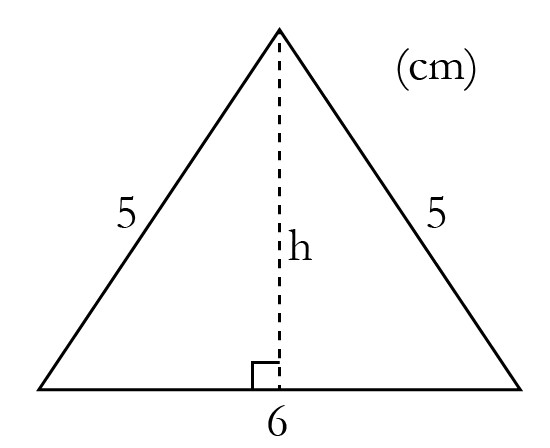
\includegraphics[scale=0.3]{images/34.png} \\
		Satsen om likbent triangel ger att den båda rätvinkliga trianglarna är kongruenta vilket medför att basen för båda är $3cm$.
		Pyth. sats ger att $h=\sqrt{5^2-3^2}=4 \Rightarrow$ arean: $6*4/2=12cm^2$ och omkretsen är $16cm$. \\ \\
		Låt benen vara $y$ och basen $x$ \\ \\
		$h=\sqrt{y^2-(x/2)^2}$ \\
		area: $\dfrac{x*h}{2}=\dfrac{x\sqrt{y^2-(x/2)^2}}{2}=12cm \Leftrightarrow x\sqrt{y^2-(x/2)^2}=24cm$ \\
		omkrets: $2y+x=16cm \Leftrightarrow x=16-2y$
		\begin{align*}
		&(16-2y)\sqrt{y^2-(8-y)^2}=24 \Leftrightarrow
		2(8-y)4\sqrt{y-4}=24 \Leftrightarrow \\
		&\Leftrightarrow (8-y)\sqrt{y-4}=3 \Rightarrow
		(y^2-16y+64)(y-4)=9 \Leftrightarrow \\
		&\Leftrightarrow y^3-4y^2-16y^2+64y+64y-256=9 \Leftrightarrow
		y^3-20y^2+128y-265=0
		\end{align*}
		Ansätter lösning med $x-5$ som faktor från ursprungsfiguren (kan lösas med polynomdivision också): \\
		\[y^3-20y^2+128y-265=(x-5)(x^2+Ax+B)=x^3+(A-5)y^2+(B-5A)y-5B\]
		Identifierar variablerna: \\
		\[\begin{cases}
		A-5=-20 \\
		B-5A=128
		\end{cases}
		\Leftrightarrow
		\begin{cases}
		A=-15 \\
		B=53
		\end{cases}\]
		\[y^3-20y^2+128y-265=(y-5)(y^2-15y+53)\] \\
		$y^2-15y+53=0$ \\
		pq-formeln: \\
		$y=\dfrac{15}{2}\pm\sqrt{\dfrac{15^2-212}{4}}=\dfrac{15\pm\sqrt{13}}{2}$ \\
		$y_1=\dfrac{15+\sqrt{13}}{2} \Rightarrow 
		x=16-15-\sqrt{13} \Rightarrow 
		x < 0 \Rightarrow$ falsk rot \\
		$y_2=\dfrac{15-\sqrt{13}}{2} \Rightarrow x=16-15+\sqrt{13}=1+\sqrt{13}$ \\ \\
		\textbf{Svar:} $x=1+\sqrt{13}$ och $y=\dfrac{15-\sqrt{13}}{2}$
	\end{quotation}
	
	\pagebreak
	\texttt{\tskcol{3.5~~~a) (s.)}}
	\begin{quotation}
		\noindent
		\begin{align*}
		&\dfrac{1}{x-1}+\dfrac{1}{x}+\dfrac{1}{x+1}=0\Leftrightarrow
		\dfrac{x(x+1)+x^2-1+x(x-1)}{x(x^2-1)}=0 \Leftrightarrow \\
		&\Leftrightarrow \dfrac{3x^2-1}{x(x^2-1)}=0\Rightarrow 
		3x^2-1=0 \Leftrightarrow 
		(\sqrt{3}x+1)(\sqrt{3}x-1)=0 \Leftrightarrow
		(x+\frac{1}{\sqrt{3}})(x-\frac{1}{\sqrt{3}})=0
		\end{align*}
		Faktorsatsen ger då: $x_1=-\frac{1}{\sqrt{3}}$ och $x_2=\frac{1}{\sqrt{3}}$
		\\ \\
		\textbf{Svar:} $x_{1,2}=\pm\frac{1}{\sqrt{3}}$
	\end{quotation}
	
	\texttt{\tskcol{~~~~~~b) (s.)}}
	\begin{quotation}
		\noindent
		\begin{align*}
		&\dfrac{1}{x-1}-\dfrac{1}{x-2}=\dfrac{1}{x-3}-\dfrac{1}{x-4}\Leftrightarrow 
		\dfrac{\cancel{x}-2-\cancel{x}+1}{(x-1)(x-2)}=\dfrac{\cancel{x}-4-\cancel{x}+3}{(x-3)(x-4)} \Leftrightarrow \\
		&\Leftrightarrow \dfrac{1}{x^2-3x+2}=\dfrac{1}{x^2-7x+12} \Rightarrow
		\cancel{x^2}-3x+2=\cancel{x^2}-7x+12 \Leftrightarrow \\
		&\Leftrightarrow x=\frac{10}{4}=\frac{5}{2}
		\end{align*}
		\\
		\textbf{Svar:} $x=\frac{5}{2}$
	\end{quotation}
	
	\texttt{\tskcol{~~~~~~c) (s.)}}
	\begin{quotation}
		\noindent
		\begin{align*}
		&\dfrac{1}{x^2-2x}+\dfrac{1}{x^2+3x}=0 \Leftrightarrow 
		\dfrac{\cancel{x}(x+3)+\cancel{x}(x-2)}{x^{\cancel{2}}(x-2)(x+3)}=0 \Rightarrow \\
		&\Rightarrow x+3+x-2=0 \Leftrightarrow
		2x+1=0 \Leftrightarrow
		x=-\frac{1}{2}
		\end{align*}
		\\
		\textbf{Svar:} $x=-\frac{1}{2}$
	\end{quotation}
	
	\pagebreak
	\texttt{\tskcol{~~~~~~d) (s.)}}
	\begin{quotation}
		\noindent
		\begin{align*}
		&\dfrac{1}{x+2}-\dfrac{x+2}{x-2}=\dfrac{x^2}{4-x^2}\Leftrightarrow
		\dfrac{x-2-(x+2)^2}{x^2-4}=\dfrac{x^2}{4-x^2} \Rightarrow \\
		& \Rightarrow (4-x^2)(-x^2-3x-6)=x^2(x^2-4) \Leftrightarrow \\
		&\Leftrightarrow -\cancel{4x^2}-12x-24+\cancel{x^4}+3x^3+6x^2=\cancel{x^4}-\cancel{4x^2} \Leftrightarrow \\
		&\Leftrightarrow x^3+2x^2-4x-8=0
		\end{align*}
		Gissar en lösning till ekvationen och hittar $x=2$. Ansätter lösning med $x-2$ som faktor (kan lösas med polynomdivision också): 
		\[x^3+2x^2-4x-8=(x-2)(x^2+Ax+B)=x^3+(A-2)x^2+(B-2A)x-2B\]
		Identifierar variabler:
		\[\begin{cases}
		A-2=2 \\
		B-2A=-4
		\end{cases}
		\Leftrightarrow
		\begin{cases}
		A=4 \\
		B=4
		\end{cases}\]
		\[(x-2)(x^2+4x+4)=0\]
		Kvadreringsregeln:
		\[(x-2)(x^2+4x+4)=0\Leftrightarrow 
		(x-2)(x+2)^2=0\]
		Faktorsatsen: $x_1=2$ och $x_{2,3}=-2$.
		Både $2$ och $-2$ är dock falska rötter då de resulterar i nolldivision i ursprungsekvationen.
		\\ \\
		\textbf{Svar:} Ekvationen saknar lösning
	\end{quotation}
	
	\texttt{\tskcol{3.6~~~~~ (s.)}}
	\begin{quotation}
		\noindent
		Formeln för hastighet, sträcka och tid är $s=v*t \Leftrightarrow t=\frac{s}{v}$. Låt $x$ vara båtens hastighet i stillastående vatten. Den totala tiden för resan är tiden dit ($t_1$) plus tiden tillbaka ($t_1$) ($t_1+t_2=t$).
		Hastigheten båten har dit ($v_1$) kan beskrivas som $x-2.4$ och hastigheten hem ($v_2$) som $x+2.4$. $t=2$ och $s=6.4$.
		\[t_1+t_2=t\Leftrightarrow
		\frac{s}{v_1}+\frac{s}{v_2}=t\] \\
		\begin{align*}
		&\frac{6.4}{x-2.4}+\frac{6.4}{x+2.4} = 2 \Leftrightarrow
		\frac{6.4(x+2.4)+6.4(x-2.4)}{(x-2.4)(x+2.4)} = 2 \Leftrightarrow \\
		&6.4(2x+\cancel{2.4-2.4})=2(x^2-2.4^2) \Leftrightarrow
		\cancel{2}*6.4x=\cancel{2}(x^2-2.4^2) \Leftrightarrow \\
		&x^2-6.4x-5.76=0
		\end{align*}
		pq-formeln:
		\[x=3.2\pm\sqrt{10.24+5.76} =3.2\pm\sqrt{16}=3.2\pm 4\]
		$x_1=7.2$ och $x_2=-0.8$. Eftersom hastigheten i uppgiften inte kan vara negativ gäller endast $x_1$
		\\ \\
		\textbf{Svar:} $7.2$ km/h 
	\end{quotation}
	
	\texttt{\tskcol{3.7~~~a) (s.)}}
	\begin{quotation}
		\noindent
		\[\sqrt{x+2}=x \Rightarrow
		x+2=x^2 \Leftrightarrow
		x^2-x-2=0 \]
		pq-formeln: \\
		\[x=\frac{1}{2}\pm\sqrt{\frac{1}{4}+\frac{8}{4}} \Leftrightarrow
		x=\frac{1}{2}\pm\frac{3}{2}\]
		$x_1=2$ \\
		$x_2=-1$ Falsk rot (sätt in i ursprungsekvationen).
		\\ \\
		\textbf{Svar:} $x=2$
	\end{quotation}
	
	\texttt{\tskcol{~~~~~~b) (s.)}}
	\begin{quotation}
		\noindent
		\[\sqrt{x+2}=-x \Rightarrow
		x+2=x^2 \Leftrightarrow
		x^2-x-2=0\]
		pq-formeln: \\
		\[x=\frac{1}{2}\pm\sqrt{\frac{1}{4}+\frac{8}{4}} \Leftrightarrow
		x=\frac{1}{2}\pm\frac{3}{2}\]
		$x_1=2$ Falsk rot (sätt in i ursprungsekvationen). \\
		$x_2=-1$
		\\ \\
		\textbf{Svar:} $x=-1$
	\end{quotation}
	
	\texttt{\tskcol{~~~~~~c) (s.)}}
	\begin{quotation}
		\noindent
		\begin{align*}
		&x-\sqrt{x-2}=4 \Leftrightarrow
		\sqrt{x-2}=x-4 \Rightarrow
		x-2=(x-4)^2 \Leftrightarrow \\
		&x-2=x^2-8x+16 \Leftrightarrow
		x^2-9x+18=0
		\end{align*}
		pq-formeln: \\
		\[x=\frac{9}{2}\pm\sqrt{\frac{81}{4}-\frac{72}{4}} \Leftrightarrow
		x=\frac{9}{2}\pm\frac{3}{2}\]
		$x_1=6$ \\
		$x_2=3$ Falsk rot (sätt in i ursprungsekvationen).
		\\ \\
		\textbf{Svar:} $x=6$
	\end{quotation}
	
	\texttt{\tskcol{3.8~~~a) (s.)}}
	\begin{quotation}
		\noindent
		\[\sqrt{x+2}=\sqrt{2x+1} \Rightarrow
		x+2=2x+1 \Leftrightarrow
		x=1\]
		\\
		\textbf{Svar:} $x=1$
	\end{quotation}
	
	\pagebreak
	\texttt{\tskcol{~~~~~~b) (s.)}}
	\begin{quotation}
		\noindent
		\[\sqrt{3x+2}=\sqrt{2x+1} \Rightarrow
		3x+2=2x+1 \Leftrightarrow
		x=-1 \text{~~~Falsk rot.}\]
		\\
		\textbf{Svar:} Ekvationen saknar lösning
	\end{quotation}
	
	\texttt{\tskcol{~~~~~~c) (s.)}}
	\begin{quotation}
		\noindent
		\[\sqrt{x+2}=\sqrt{x} \Rightarrow
		x+2=x \Leftrightarrow
		2=0 \text{~~~Ej ekvivalent.}\]
		\\
		\textbf{Svar:} Ekvationen saknar lösning
	\end{quotation}
		
	\texttt{\tskcol{~~~~~~d) (s.)}}
	\begin{quotation}
		\noindent
		\[\sqrt{x-2}\sqrt{x+3}=x \Rightarrow
		(x-2)(x+3)=x^2 \Leftrightarrow
		\cancel{x^2}+x-6=\cancel{x^2} \Leftrightarrow
		x=6\]
		\\
		\textbf{Svar:} $x=6$
	\end{quotation}
	
	\texttt{\tskcol{~~~~~~e) (s.)}}
	\begin{quotation}
		\noindent
		\begin{align*}
		&(3-\sqrt{x})(3+\sqrt{x})=8\sqrt{x} \Leftrightarrow
		9-x=8\sqrt{x} \Rightarrow \\
		&\Rightarrow x^2-18x+81=64x \Leftrightarrow
		x^2-82x+81=0
		\end{align*}
		pq-formeln: \\
		\[x=41\pm\sqrt{41^2-81}=41\pm40\]
		$x_1=81$ falsk rot. \\
		$x_2=1$
		\\ \\
		\textbf{Svar:} $x=1$
	\end{quotation}
		
	\texttt{\tskcol{~~~~~~f) (s.)}}
	\begin{quotation}
		\noindent
		\begin{align*}
		&\sqrt{x}=\dfrac{3}{\sqrt{x}}+\sqrt{3+x} \Leftrightarrow
		x=3+\sqrt{x(3+x)} \Leftrightarrow
		x-3=\sqrt{3x+x^2} \Rightarrow \\
		&\Rightarrow \cancel{x^2}-6x+9=3x+\cancel{x^2} \Leftrightarrow
		9x=9 \Leftrightarrow
		x=1 \text{~~~Falsk rot.}
		\end{align*}
		\\
		\textbf{Svar:} Lösning saknas
	\end{quotation}
	
	\subsection*{Ekvationer}
	
	\texttt{\tskcol{3.9~~~~~ (s.)}}
	\begin{quotation}
		\noindent
		$2<3 \Leftarrow$ är ''2 \textbf{mindre} än 3''? Ja \\
		$2 \le 3 \Leftarrow$ är ''2 \textbf{mindre} eller lika med 3''? Ja \\
		$2 \le 2 \Leftarrow$ är ''2 mindre eller \textbf{lika med} 2''? Ja 
		\\ \\
		\textbf{Svar:} Alla tre
	\end{quotation}
	
	\texttt{\tskcol{3.10~~~~ (s.)}}
	\begin{quotation}
		\noindent
		Nedan visar jag min tankeprocess för att lösa uppgiften.
		\[\frac{2}{0.02}=
		\frac{2}{2}*\frac{1}{10^{-2}}=
		1*10^2=
		100\]
		\[\frac{31}{0.2}=
		\frac{31}{2}*\frac{1}{10^{-1}}=
		15.5*10=
		155\]
		\[\frac{0.00009}{0.000006}=
		\frac{9}{6}*\frac{10^{-5}}{10^{-6}}=
		1.5*10=
		15\]
		\\ \\
		\textbf{Svar:} $\dfrac{0.00009}{0.000006}<\dfrac{2}{0.02}<\dfrac{31}{0.2}$
	\end{quotation}
	
	\texttt{\tskcol{3.11~~a) (s.)}}
	\begin{quotation}
		\noindent
		$3x+1<2 \Leftrightarrow
		3x<1 \Leftrightarrow
		x<\frac{1}{3}$
		\\ \\
		\textbf{Svar:} $x<\frac{1}{3}$
	\end{quotation}
	
	\texttt{\tskcol{~~~~~~b) (s.)}}
	\begin{quotation}
		\noindent
		$-3x+2\le1 \Leftrightarrow
		-3x\le-1 \Leftrightarrow
		x\ge\frac{1}{3}$
		\\ \\
		\textbf{Svar:} $x\ge\frac{1}{3}$
	\end{quotation}
	
	\texttt{\tskcol{~~~~~~c) (s.)}}
	\begin{quotation}
		\noindent
		$3x+1>4x+5 \Leftrightarrow
		x<-4$
		\\ \\
		\textbf{Svar:} $x<-4$
	\end{quotation}
	
	\texttt{\tskcol{~~~~~~d) (s.)}}
	\begin{quotation}
		\noindent
		$(x-3)(x+3)\le x^2 \Leftrightarrow
		\cancel{x^2}-9 \le \cancel{x^2} \Leftrightarrow
		-9 \le 0 \Rightarrow x\in\mathbb{R}$
		\\ \\
		\textbf{Svar:} $x\in\mathbb{R}$
	\end{quotation}
	
	\pagebreak
	\texttt{\tskcol{3.12~~a) (s.)}}
	\begin{quotation}
		\noindent
		Använd en teckentabell och hitta intervallet/n som ger positiva värden.
		
		 \[\dfrac{x+4}{x-1}>0\] \\
		\begin{tabular}{c|c|c|c|c|c}
			$x$ & & $-4$ & & $1$ & \\ \hline
			$x+4$              & $-$ & $0$ & $+$ & $+$ & $+$ \\
			$x-1$              & $-$ & $-$ & $-$ & $0$ & $+$ \\ \hline
			$\dfrac{x+4}{x-1}$ & $+$ & $0$ & $-$ &$\wr$& $+$ 
		\end{tabular} \\ \\
		\textbf{Svar:} $x>1$ eller $x<-4$
	\end{quotation}
	
	\texttt{\tskcol{~~~~~~b) (s.)}}
	\begin{quotation}
		\noindent
		Utnyttja teckentabellen i förra uppgiften men ta intervallet som ger negativa värden.
		
		\[\dfrac{x+4}{x-1}<0\]
		\\
		\textbf{Svar:} teckentabellen i \texttt{\tskcol{a)}} ger: $-4<x<1$
	\end{quotation}
	
	\texttt{\tskcol{~~~~~~c) (s.)}}
	\begin{quotation}
		\noindent
		Använd en teckentabell och hitta intervallet/n som ger negativa värden.
		\[\dfrac{x+1}{x(x-1)}<0\] \\
		\begin{tabular}{c|c|c|c|c|c|c|c}
			$x$ & & $-1$ & & $0$ & & $1$ & \\ \hline
			$x+1$                  & $-$ & $0$ & $+$ & $+$ & $+$ & $+$ & $+$ \\
			$x$                    & $-$ & $-$ & $-$ & $0$ & $+$ & $+$ & $+$ \\
			$x-1$                  & $-$ & $-$ & $-$ & $-$ & $-$ & $0$ & $+$ \\ \hline
			$\dfrac{x+1}{x(x-1)}$  & $-$ & $0$ & $+$ &$\wr$& $-$ &$\wr$& $+$ \\
		\end{tabular}
		\\ \\
		\textbf{Svar:} $x<-1$ eller $0<x<1$
	\end{quotation}
	
	\texttt{\tskcol{~~~~~~d) (s.)}}
	\begin{quotation}
		\noindent
		Använd en teckentabell och hitta intervallet/n som ger positiva värden.
		\[(x+2)(2x-1) > 0\] \\
		\begin{tabular}{c|c|c|c|c|c}
			$x$ & & $-2$ & & $1/2$ & \\ \hline
			$x+2$         & $-$ & $0$ & $+$ & $+$ & $+$ \\
			$2x-1$        & $-$ & $-$ & $-$ & $0$ & $+$ \\ \hline
			$(x+2)(2x-1)$ & $+$ & $0$ & $-$ &$\wr$& $+$ 
		\end{tabular}
		\\ \\
		\textbf{Svar:} $x<-2$ eller $x>1/2$
	\end{quotation}
	
	\pagebreak
	\texttt{\tskcol{3.13~~~~ (s.)}}
	\begin{quotation}
		\noindent
		Skriv om olikheten så att högerledet blir noll och allt i vänsterledet hamnar på samma bråkstreck. Använd sedan en teckentabell och hitta intervallet/n som ger negativa värden.
		
		\[\dfrac{3x+1}{x+2}<2 \Leftrightarrow
		\dfrac{3x+1-2(x+2)}{x+2}<0 \Leftrightarrow
		\dfrac{x-3}{x+2}<0\] \\
		\begin{tabular}{c|c|c|c|c|c}
			$x$ & & $-2$ & & $3$ & \\ \hline
			$x-3$              & $-$ & $-$ & $-$ & $0$ & $+$ \\
			$x+2$              & $-$ & $0$ & $+$ & $+$ & $+$ \\ \hline
			$\dfrac{x-3}{x+2}$ & $+$ &$\wr$& $-$ & $0$ & $+$ 
		\end{tabular}
		\\ \\
		\textbf{Svar:} $-2<x<3$
	\end{quotation}
	
	\texttt{\tskcol{3.14~~a) (s. 44-45)}}
	\begin{quotation}
		\noindent
		Se sidorna 44-45 i läroboken för förklaring till varför det fungerar såhär.
		\[\dfrac{x^2+1}{x}<x\]
		\begin{align*}
		&\text{om } x>0\text{:} &\dfrac{x^2+1}{x}<x &\Leftrightarrow &\cancel{x^2}+1<\cancel{x^2} &\Leftrightarrow &1<0 \\
		&\text{om } x<0\text{:} &\dfrac{x^2+1}{x}<x &\Leftrightarrow &\cancel{x^2}+1>\cancel{x^2} &\Leftrightarrow &1>0
		\end{align*}
		$1<0$ är alltid sant vilket innebär att skillnaden gäller för alla $x$ mindre än noll.
		\\ \\
		\textbf{Svar:} $x<0$ 
	\end{quotation}
	
	\texttt{\tskcol{~~~~~~b) (s.)}}
	\begin{quotation}
		\noindent
		Skriv om olikheten så att högerledet blir noll och allt i vänsterledet hamnar på samma bråkstreck. Använd sedan en teckentabell och hitta intervallet/n som ger negativa värden.
		\[\dfrac{2x^2}{x+2}<x-2 \Leftrightarrow
		\dfrac{2x^2-(x+2)(x-2)}{x+2}<0 \Leftrightarrow\]
		\[\Leftrightarrow \dfrac{\cancel{2}x^2-\cancel{x^2}+4}{x+2}<0 \Leftrightarrow
		\dfrac{x^2+4}{x+2}<0\] \\
		\begin{tabular}{c|c|c|c}
			$x$ & & $-2$ & \\ \hline
			$x^2+4$              & $+$ & $+$ & $+$ \\
			$x+2$                & $-$ & $0$ & $+$ \\ \hline
			$\dfrac{x^2+4}{x+2}$ & $-$ &$\wr$& $+$ 
		\end{tabular}
		\\ \\
		\textbf{Svar:} $x<-2$
	\end{quotation}
	
	\pagebreak
	\texttt{\tskcol{~~~~~~c) (s.)}}
	\begin{quotation}
		\noindent
		Eftersom $x^2$ aldrig kan bli negativt behövs inget motsvarade det i uppgift \texttt{\tskcol{a)}} göras.
		\[\dfrac{x^2+2}{x^2+1}>1 \Leftrightarrow
		\cancel{x^2}+2>\cancel{x^2}+1 \Leftrightarrow
		2>1\]
		\\
		\textbf{Svar:} Alla $x$
	\end{quotation}
	
	\texttt{\tskcol{3.15~~a) (s.)}}
	\begin{quotation}
		\noindent
		Skriv om olikheten så att allt är i vänsterledet och använd konjugatregeln baklänges. Använd sedan en teckentabell och hitta intervallet/n som ger negativa värden.
		\[x^2<4 \Leftrightarrow
		x^2-4<0 \Leftrightarrow
		(x+2)(x-2)<0\] \\
		\begin{tabular}{c|c|c|c|c|c}
			$x$ & & $-2$ & & $2$ & \\ \hline
			$x+2$        & $-$ & $0$ & $+$ & $+$ & $+$ \\
			$x-2$        & $-$ & $-$ & $-$ & $0$ & $+$ \\ \hline
			$(x+2)(x-2)$ & $+$ & $0$ & $-$ & $0$ & $+$ 
		\end{tabular}
		\\ \\
		\textbf{Svar:} $-2<x<2$
	\end{quotation}
	
	\texttt{\tskcol{~~~~~~b) (s.)}}
	\begin{quotation}
		\noindent
		Utnyttja teckentabellen i förra uppgiften men ta intervallet som ger positiva värden.
		\\ \\
		\textbf{Svar:} teckentabellen i \texttt{a)} ger: $x<-2$ eller $x>2$
	\end{quotation}
	
	\texttt{\tskcol{~~~~~~c) (s.)}}
	\begin{quotation}
		\noindent
		Använd kvadreringsregeln och lös olikheten.
		\[(x+1)^2>(x+5)^2 \Leftrightarrow
		\cancel{x^2}+2x+1>\cancel{x^2}+10x+25\Leftrightarrow \]
		\[\Leftrightarrow -24>8x \Leftrightarrow
		x<-3\]
		\\
		\textbf{Svar:} $x<-3$ 
	\end{quotation}
	
	\pagebreak
	\texttt{\tskcol{3.16~~~~ (s.)}}
	\begin{quotation}
		\noindent
		Förenkla vänsterledet, flytta över ettan och skriv allt på ett gemensamt bråkstreck. Använd sedan en teckentabell och hitta intervallet/n som ger negativa värden.
		\[\dfrac{1-x^4}{1-(x^2+1)^2}<1 \Leftrightarrow
		\dfrac{1-x^4}{1-x^4-2x^2-1}<1 \Leftrightarrow
		\dfrac{1-x^4}{-x^4-2x^2}<1 \Leftrightarrow\]
		\[\Leftrightarrow \dfrac{1-x^4-(-x^4-2x^2)}{-x^2(x^2+2)}<0 \Leftrightarrow
		\dfrac{2x^2+1}{-x^2(x^2+2)}<0\]
		\begin{tabular}{c|c|c|c}
			$x$ & & $0$ & \\ \hline
			$2x^2+1$                      & $+$ & $+$ & $+$ \\
			$-x^2$                        & $-$ & $0$ & $-$ \\
			$x^2+2$                       & $+$ & $+$ & $+$ \\ \hline
			$\dfrac{2x^2+1}{-x^2(x^2+2)}$ & $-$ &$\wr$& $-$ 
		\end{tabular}
		\\ \\
		\textbf{Svar:} $x\neq 0$
	\end{quotation}
	
	\texttt{\tskcol{3.17~~a) (s.)}}
	\begin{quotation}
		\noindent
		Lös ekvationen genom att multiplicera termerna med $x$. Faktorisera sedan täljaren. Notera att grundekvationen inte är definierad för $x=0$ därför implicerar endast den första ekvationen den andra.
		\[x+\dfrac{4}{x}=5 \Rightarrow
		x^2+4=5x \Leftrightarrow
		x^2-5x+4=0 \Leftrightarrow
		(x-4)(x-1)=0\]
		Faktorsatsen ger:
		$x_1=4$, $x_2=1$
		\\ \\
		\textbf{Svar:} $x_1=4$, $x_2=1$
	\end{quotation}
	
	\texttt{\tskcol{~~~~~~b) (s.)}}
	\begin{quotation}
		\noindent
		Skriv om olikheten så alla termer står på samma bråkstreck i vänsterledet. Använd sedan en teckentabell och hitta intervallet/n som ger positiva värden.
		\[x+\dfrac{4}{x}>5 \Leftrightarrow
		\dfrac{x^2+4}{x}>5 \Leftrightarrow
		\dfrac{x^2-5x+4}{x}>0 \Leftrightarrow
		\dfrac{(x-4)(x-1)}{x}>0\]
		\begin{tabular}{c|c|c|c|c|c|c|c}
			$x$                      &     & $0$ &     & $1$ &     & $4$ &     \\ \hline
			$x-4$                    & $-$ & $-$ & $-$ & $-$ & $-$ & $0$ & $+$ \\
			$x-1$                    & $-$ & $-$ & $-$ & $0$ & $+$ & $+$ & $+$ \\
			$x$                      & $-$ & $0$ & $+$ & $+$ & $+$ & $+$ & $+$ \\ \hline
			$\dfrac{(x-4)(x-1)}{x}$  & $-$ &$\wr$& $+$ & $0$ & $-$ & $0$ & $+$ \\
		\end{tabular}
		\\ \\
		\textbf{Svar:} $0<x<1$ eller $x>4$
	\end{quotation}
	
	\pagebreak
	\section*{Kapitel 4: Summor och talföljder}
	\subsection*{Summatecken}
	
	\texttt{\tskcol{4.1~~~a) (s.)}}
	\begin{quotation}
		\noindent
		\[\sum_{n=1}^{5}n^3=1^3+2^3+3^3+4^3+5^3=
		1+8+27+64+125=
		225\]
		\\
		\textbf{Svar:} $225$
	\end{quotation}
	
	\texttt{\tskcol{~~~~~~b) (s.)}}
	\begin{quotation}
		\noindent
		\[\sum_{k=0}^{4}(k^2-3k)=
		0^2-3*0+1^2-3*1+2^2-3*2+3^2-3*3+4^2-3*4=\]
		\[=1-3+4-6+9-9+16-12=0\]
		\\
		\textbf{Svar:} $0$
	\end{quotation}
	
	\texttt{\tskcol{~~~~~~c) (s.)}}
	\begin{quotation}
		\noindent
		\[\sum_{k=2}^{100}3=\underbrace{3+3+\ldots+3+3}_\text{99 st.}=
		3*99=
		297\]
		\\
		\textbf{Svar:} $297$
	\end{quotation}
	
	\texttt{\tskcol{~~~~~~d) (s.)}}
	\begin{quotation}
		\noindent
		Antalet element kommer alltid vara lika med övre gränsen minus undre gränsen plus ett.
		\[\sum_{k=m}^{n}3=3(n-m+1)\]
		\\
		\textbf{Svar:} $3(n-m+1)$
	\end{quotation}
	
	\texttt{\tskcol{4.2~~~a) (s.)}}
	\begin{quotation}
		\noindent
		\[\underbrace{1+\frac{1}{2}+\frac{1}{3}+\ldots+\frac{1}{10}}_\text{10 st. från 1 till 10}=
		\sum_{k=1}^{10}\frac{1}{k}\]
		\\
		\textbf{Svar:} $\displaystyle\sum_{k=1}^{10}\frac{1}{k}$
	\end{quotation}
	
	\texttt{\tskcol{~~~~~~b) (s.)}}
	\begin{quotation}
		\noindent
		\[\underbrace{2*3+3*4+4*5+\ldots+n(n+1)}_\text{från 2 till n}=
		\sum_{k=2}^{n}k(k+1)\]
		\\
		\textbf{Svar:} $\displaystyle\sum_{k=2}^{n}k(k+1)$
	\end{quotation}
	
	\texttt{\tskcol{~~~~~~c) (s.)}}
	\begin{quotation}
		\noindent
		Hitta mönstret och skriv om så det kan skrivas med summatecken.
		\[1+3+9+27+81+243=
		\underbrace{3^0+3^1+3^2+3^3+3^4+3^5}_\text{6 st. från 0 till 5}=
		\sum_{k=0}^{5}3^k\]
		\\
		\textbf{Svar:} $\displaystyle\sum_{k=0}^{5}3^k$
	\end{quotation}
	
	\subsection*{Aritmetisk summa}
	
	\texttt{\tskcol{4.3~~~~~ (s.)}}
	\begin{quotation}
		\noindent
		Se formeln för aritmetisk summa.
		\[1+2+\ldots+100=\sum_{k=1}^{100}k=\frac{100(100+1)}{2}=5050\]
		\\
		\textbf{Svar:} $5050$
	\end{quotation}
	
	\texttt{\tskcol{4.4~~~~~ (s.)}}
	\begin{quotation}
		\noindent
		Hitta mönstret och skriv om så det går att skrivas med summatecken.
		\[3+6+\ldots+96+99=
		3*1+3*2+\ldots+3*32+3*33=\]
		\[=3\underbrace{(1+2+\ldots+33+44)}_\text{33 st. från 1 till 33}=
		3\sum_{k=1}^{33}k=
		3*\frac{33*34}{2}=
		1683\]
		\\
		\textbf{Svar:} $1683$
	\end{quotation}
	
	\texttt{\tskcol{4.5~~~a) (s.)}}
	\begin{quotation}
		\noindent
		\[1+2+3+\ldots+9+10=\sum_{k=1}^{10}k=\frac{10*11}{2}=55\]
		\\
		\textbf{Svar:} $55$
	\end{quotation}
	
	\pagebreak
	\texttt{\tskcol{~~~~~~b) (s.)}}
	\begin{quotation}
		\noindent
		bryt ut fyran och skriv om med summatecken.
		\[4+8+12+\ldots+36+40=4(1+2+3+\ldots+9+10)=4\sum_{k=1}^{10}k=4*\frac{10*11}{2}=220\]
		\\
		\textbf{Svar:} $220$
	\end{quotation}
	
	\texttt{\tskcol{~~~~~~c) (s.)}}
	\begin{quotation}
		\noindent
		Dela upp serien och inse att den kan delas upp i två separata summor och att fyran kan brytas ut.
		\begin{align*}
		&3+7+11+\ldots+35+39= \\
		&=(4*1-1)+(4*2-1)+(4*3-1)+\ldots+(4*9-1)+(4*10-1)= \\
		&=4(1+2+3+\ldots+9+10)-(\underbrace{1+1+1\ldots+1+1}_\text{10 st.})= \\
		&=4\sum_{k=1}^{10}k-\sum_{k=1}^{10}1=
		4*\frac{10*11}{2}-10*1=
		210
		\end{align*} 
		\\
		\textbf{Svar:} $210$
	\end{quotation}
	
	\texttt{\tskcol{~~~~~~d) (s.)}}
	\begin{quotation}
		\noindent
		Dela upp serien och inse att den kan delas upp i två separata summor och att tian kan brytas ut.
		\begin{align*}
		&-3+7+17+\ldots+87+97= \\
		&=(10*0-3)+(10*1-3)+(10*2-3)+\ldots+(10*9-3)+(10*10-3)= \\
		&=10(0+1+2+\ldots+9+10)-(\underbrace{3+3+3\ldots+3+3}_\text{11 st.})= \\
		&=10\sum_{k=0}^{10}k-\sum_{k=0}^{10}3=
		10(0+\sum_{k=1}^{10}k)-\sum_{k=0}^{10}3
		10*\frac{10*11}{2}-11*3=
		517
		\end{align*} 
		\\
		\textbf{Svar:} $517$
	\end{quotation}
	
	\texttt{\tskcol{4.6~~~a) (s.)}}
	\begin{quotation}
		\noindent
		Bryt ut trean och använd aritmetisk summa.
		\begin{align*}
		&\sum_{k=1}^{15}3k=
		3*1+3*2+\ldots+3*14+3*15= \\
		&=3(1+2+\ldots+14+15)=
		3\sum_{k=1}^{15}k=
		3\frac{15*16}{2}=
		360
		\end{align*}
		\\
		\textbf{Svar:} $360$
	\end{quotation}
	
	\texttt{\tskcol{~~~~~~b) (s.)}}
	\begin{quotation}
		\noindent
		Bryt ut trean och två och använd aritmetisk summa.
		\begin{align*}
		&\sum_{k=1}^{15}(3k+2)=
		(3*1+2)+(3*2+2)+\ldots+(3*14+2)+(3*15+2)= \\
		&=3(1+2+\ldots+14+15)+(\underbrace{2+2+\ldots+2+2}_\text{15 st.})=
		3\sum_{k=1}^{15}k+\sum_{k=1}^{15}2= \\
		&=3\frac{15*16}{2}+2*15=
		390
		\end{align*}
		\\
		\textbf{Svar:} $390$
	\end{quotation}
	
	\texttt{\tskcol{~~~~~~c) (s.)}}
	\begin{quotation}
		\noindent
		Bryt ut trean och två som i förra uppgiften och använd aritmetisk summa.
		\begin{align*}
		&\sum_{k=1}^{n}(3k+2)=
		3(1+2+\ldots+(n-1)+n)+(\underbrace{2+2+\ldots+2+2}_\text{n st.})= \\
		&=3\sum_{k=1}^{n}k+\sum_{k=1}^{n}2=
		3\frac{n(n+1)}{2}+2n
		\end{align*}
		\\
		\textbf{Svar:} $3\dfrac{n(n+1)}{2}+2n$
	\end{quotation}
	
	\texttt{\tskcol{~~~~~~d) (s.)}}
	\begin{quotation}
		\noindent
		Bryt ut $a$ och $d$ som i förra uppgiften och använd aritmetisk summa.
		\begin{align*}
		&\sum_{k=1}^{n}(ak+d)=
		a(1+2+\ldots+(n-1)+n)+(\underbrace{d+d+\ldots+d+d}_\text{n st.})= \\
		&=a\sum_{k=1}^{n}k+\sum_{k=1}^{n}d=
		a\frac{n(n+1)}{2}+dn
		\end{align*}
		\\
		\textbf{Svar:} $a\dfrac{n(n+1)}{2}+dn$
	\end{quotation}
	
	\subsection*{Geometrisk summa}
	
	\texttt{\tskcol{4.7~~~a) (s.)}}
	\begin{quotation}
		\noindent
		Skriv om termerna så att de kan skrivas som en geometrisk summa. Använd sedan formeln för geometrisk summa.
		\[1+2+4+8+16+32=
		2^0+2^1+2^2+2^3+2^4+2^5=
		\sum_{k=0}^{5}2^k=
		\frac{2^{5+1}-1}{2-1}=
		127\]
		\\
		\textbf{Svar:} $127$
	\end{quotation}
	
	\texttt{\tskcol{~~~~~~b) (s.)}}
	\begin{quotation}
		\noindent
		Skriv om termerna så att de kan skrivas som en geometrisk summa. Använd sedan formeln för geometrisk summa.
		\begin{align*}
		&1-3+9-27+81-243=
		(-3)^0+(-3)^1+(-3)^2+(-3)^3+(-3)^4+(-3)^5= \\
		&=\sum_{k=0}^{5}(-3)^k=
		\frac{(-3)^{5+1}-1}{-3-1}=
		-182
		\end{align*}
		\\
		\textbf{Svar:} $-182$
	\end{quotation}
	
	\texttt{\tskcol{~~~~~~c) (s.)}}
	\begin{quotation}
		\noindent
		Skriv om termerna så att de kan skrivas som en geometrisk summa. Eftersom start värdet inte är $0$ finns det två olika sätt att lösa det på: antingen göra en summa av delmängden där $k \ge 0$ och addera resten efteråt eller genom att bryta ut den minsta exponenten.
		\begin{align*}
		&2+1+\frac{1}{2}+\frac{1}{4}+\ldots+\frac{1}{128}=
		2+\left(\tfrac{1}{2}\right)^0+\left(\tfrac{1}{2}\right)^1+\left(\tfrac{1}{2}\right)^2+\ldots+\left(\tfrac{1}{2}\right)^7= \\
		&=2+\sum_{k=0}^{7}\left(\tfrac{1}{2}\right)^k=
		2+\frac{\left(\frac{1}{2}\right)^8-1}{\frac{1}{2}-1}=
		\frac{511}{128}
		\end{align*}
		eller \begin{align*}
		&2+1+\frac{1}{2}+\frac{1}{4}+\ldots+\frac{1}{128}=
		\left(\tfrac{1}{2}\right)^{-1}+\left(\tfrac{1}{2}\right)^0+\left(\tfrac{1}{2}\right)^1+\left(\tfrac{1}{2}\right)^2+\ldots+\left(\tfrac{1}{2}\right)^7= \\
		&=\left(\tfrac{1}{2}\right)^{-1}*\left(\left(\tfrac{1}{2}\right)^0+\left(\tfrac{1}{2}\right)^1+\left(\tfrac{1}{2}\right)^2+\ldots+\left(\tfrac{1}{2}\right)^8\right)= \\
		&=\left(\tfrac{1}{2}\right)^{-1}*\sum_{k=0}^{8}\left(\tfrac{1}{2}\right)^k=
		\left(\tfrac{1}{2}\right)^{-1}*\frac{\left(\frac{1}{2}\right)^9-1}{\frac{1}{2}-1}=
		\frac{511}{128}
		\end{align*}
		\\
		\textbf{Svar:} $\dfrac{511}{128}$
	\end{quotation}
	
	\pagebreak
	\texttt{\tskcol{~~~~~~d) (s.)}}
	\begin{quotation}
		\noindent
		Två alternativa sätt att lösa det: Bryta ut $e$ så att summan får startvärdet $0$ eller använd subtraktion så att summan kan skrivas med $0$ som startvärde.
		\begin{align*}
		e+e^2+e^3+\ldots+e^{10}=
		e(e^0+e^1+e^2+\ldots+e^9)=
		e\sum_{k=0}^{9}e^k=
		e*\frac{e^{10}-1}{e-1}
		\end{align*}
		eller
		\begin{align*}
		&e+e^2+e^3+\ldots+e^{10}=
		\sum_{k=1}^{10}e^k=
		\sum_{k=0}^{10}e^k-\sum_{k=0}^{0}e^k=
		\frac{e^{11}-1}{e-1}-\frac{e^1-1}{e-1}= \\
		&=\frac{e^{11}-\cancel{1}-(e-\cancel{1})}{e-1}=
		e*\frac{e^{10}-1}{e-1}
		\end{align*}
		\\ \\
		\textbf{Svar:} $e*\dfrac{e^{10}-1}{e-1}$
	\end{quotation}
	
	\texttt{\tskcol{~~~~~~e) (s.)}}
	\begin{quotation}
		\noindent
		Skriv om termerna så att de kan skrivas som en geometrisk summa. Använd sedan formeln för geometrisk summa.
		\begin{align*}
		&1-x+x^2-x^3+\ldots-x^9=
		(-x)^0+(-x)^1+(-x)^2+(-x)^3+\ldots++(-x)^9= \\
		&=\sum_{k=0}^{9}(-x)^k=
		\frac{(-x)^{10}-1}{-x-1}=
		-\frac{x^{10}-1}{x+1}=
		\frac{1-x^{10}}{x+1}
		\end{align*}
		\\
		\textbf{Svar:} $\dfrac{1-x^{10}}{x+1}$
	\end{quotation}
	
	\texttt{\tskcol{4.8~~~a) (s.)}}
	\begin{quotation}
		\noindent
		Se \texttt{\tskcol{4.6 a)}} för resonemang kring varför faktorn $3$ kan brytas ut.
		\[\sum_{k=0}^{10}(3*2^k)=
		3*\sum_{k=0}^{10}2^k=
		3*\frac{2^{11}-1}{2-1}=
		3(2^{11}-1)\]
		\\
		\textbf{Svar:} $3(2^{11}-1)$
	\end{quotation}
	
	\pagebreak
	\texttt{\tskcol{~~~~~~b) (s.)}}
	\begin{quotation}
		\noindent
		Bryt ut en tvåa från summan eller subtrahera en kompletterande summa. 
		\begin{align*}
		&\sum_{k=1}^{10}(3*2^k)=
		3*\sum_{k=1}^{10}2^k=
		3*2(2^0+2^1+\ldots+2^9)= \\
		&=6*\sum_{k=0}^{9}2^k=
		6*\frac{2^{10}-1}{2-1}=
		6(2^{10}-1)
		\end{align*}
		eller
		\begin{align*}
		&\sum_{k=1}^{10}(3*2^k)=
		3*\sum_{k=1}^{10}2^k=
		3\left(\sum_{k=0}^{10}2^k-\sum_{k=0}^{0}2^k\right)= \\
		&=3\left(\frac{2^{11}-\cancel{1}}{2-1}-\frac{2^1-\cancel{1}}{2-1}\right)=
		3(2^{11}-2)=
		6(2^{10}-1)
		\end{align*}
		\\
		\textbf{Svar:} $6(2^{10}-1)$
	\end{quotation}
	
	\texttt{\tskcol{~~~~~~c) (s.)}}
	\begin{quotation}
		\noindent
		Bryt ut tre tvåor från summan eller subtrahera en kompletterande summa. 
		\begin{align*}
		&\sum_{k=3}^{10}(3*2^k)=
		3*\sum_{k=3}^{10}2^k=
		3*2^3(2^0+2^1+\ldots+2^7)= \\
		&=24*\sum_{k=0}^{7}2^k=
		24*\frac{2^{8}-1}{2-1}=
		24(2^{8}-1)
		\end{align*}
		eller
		\begin{align*}
		&\sum_{k=3}^{10}(3*2^k)=
		3*\sum_{k=3}^{10}2^k=
		3\left(\sum_{k=0}^{10}2^k-\sum_{k=0}^{2}2^k\right)= \\
		&=3\left(\frac{2^{11}-\cancel{1}}{2-1}-\frac{2^3-\cancel{1}}{2-1}\right)=
		3(2^{11}-2^3)=
		24(2^{10}-1)
		\end{align*}
		\\
		\textbf{Svar:} $24(2^{10}-1)$
	\end{quotation}
	
	\pagebreak
	\texttt{\tskcol{~~~~~~d) (s.)}}
	\begin{quotation}
		\noindent
		Bryt ut $m$ tvåor från summan eller subtrahera en kompletterande summa. 
		\begin{align*}
		&\sum_{k=m}^{n}(3*2^k)=
		3*\sum_{k=m}^{n}2^k=
		3*2^m(2^0+2^1+\ldots+2^{n-m})= \\
		&=3*2^m*\sum_{k=0}^{n-m}2^k=
		3*2^m*\frac{2^{n-m+1}-1}{2-1}=
		3*2^m(2^{n-m+1}-1)
		\end{align*}
		eller
		\begin{align*}
		&\sum_{k=m}^{n}(3*2^k)=
		3*\sum_{k=m}^{n}2^k=
		3\left(\sum_{k=0}^{n}2^k-\sum_{k=0}^{m-1}2^k\right)= \\
		&=3\left(\frac{2^{n+1}-\cancel{1}}{2-1}-\frac{2^{m}-\cancel{1}}{2-1}\right)=
		3(2^{n+1}-2^m)=
		3*2^m(2^{n-m+1}-1)
		\end{align*}
		\\
		\textbf{Svar:} $3*2^m(2^{n-m+1}-1)$
	\end{quotation}
	
	\texttt{\tskcol{4.9~~~a) (s.)}}
	\begin{quotation}
		\noindent
		Skriv om den negativa exponenten som ett bråktal.
		\begin{align*}
		&\sum_{k=0}^{n}(3*2^{-k})=
		3*\sum_{k=0}^{n}(2^{-k})=
		3*\sum_{k=0}^{n}\left(\tfrac{1}{2}\right)^{k}=
		3*\frac{(\frac{1}{2})^{n+1}-1}{\frac{1}{2}-1}= \\
		&=3*\frac{(\frac{1}{2})^{n+1}-1}{-\frac{1}{2}}=
		-6\left(\frac{1}{2^{n+1}}-1\right)=
		6\left(1-\frac{1}{2^{n+1}}\right)
		\end{align*}
		\\
		\textbf{Svar:} $6\left(1-\frac{1}{2^{n+1}}\right)$
	\end{quotation}
	
	\texttt{\tskcol{~~~~~~b) (s.)}}
	\begin{quotation}
		\noindent
		Skriv om den negativa exponenten som ett bråktal och fixa till så att startvärdet är noll (båda metoderna i \texttt{\tskcol{4.8 b)-c)}} går att använda).
		\begin{align*}
		&\sum_{k=1}^{n}e^{-k}=
		\sum_{k=1}^{n}\left(\tfrac{1}{e}\right)^k=
		\tfrac{1}{e}(\left(\tfrac{1}{e}\right)^0+\left(\tfrac{1}{e}\right)^1+\ldots+\left(\tfrac{1}{e}\right)^{n-1})= \\
		&=\tfrac{1}{e}*\sum_{k=0}^{n-1}\left(\tfrac{1}{e}\right)^k=
		\tfrac{1}{e}*\frac{\left(\frac{1}{e}\right)^n-1}{\frac{1}{e}-1}=
		\frac{\left(\frac{1}{e}\right)^n-1}{\frac{e}{e}-e}=
		\frac{\left(\frac{1}{e}\right)^n-1}{1-e}=
		\frac{1-\left(\frac{1}{e}\right)^n}{e-1}
		\end{align*}
		\\
		\textbf{Svar:} $\dfrac{1-\left(\frac{1}{e}\right)^n}{e-1}$
	\end{quotation}
	
	\texttt{\tskcol{~~~~~~c) (s.)}}
	\begin{quotation}
		\noindent
		Använd geometrisk summa.
		\begin{align*}
		&\sum_{n=0}^{100}(1000*(1.05)^n)=
		1000*\sum_{n=0}^{100}1.05^n=
		1000*\frac{1.05^{n+1}-1}{1.05-1}= \\
		&=1000*\frac{1.05^{n+1}-1}{\frac{1}{20}}=
		20*1000*\frac{1.05^{n+1}-1}{1}=
		20000(1.05^n+1-1)
		\end{align*}
		\\
		\textbf{Svar:} $20000(1.05^n+1-1)$
	\end{quotation}
	
	\texttt{\tskcol{~~~~~~d) (s.)}}
	\begin{quotation}
		\noindent
		Använd geometrisk summa.
		\begin{align*}
		&1-\frac{1}{2}+\frac{1}{4}-\frac{1}{8}+\ldots+\frac{1}{2^{2n}}=
		(-\tfrac{1}{2})^0+(-\tfrac{1}{2})^1+(-\tfrac{1}{2})^2+(-\tfrac{1}{2})^3+\ldots+(-\tfrac{1}{2})^{2n}= \\
		&=\sum_{k=0}^{2n}(-\tfrac{1}{2})^k=
		\frac{(-\frac{1}{2})^{2n+1}-1}{-\frac{1}{2}-1}=
		-2\frac{-\frac{1}{2^{2n+1}}-1}{3}=
		\frac{\frac{2}{2^{2n+1}}+2}{3}=
		\frac{2^{-2n}+2}{3}
		\end{align*}
		\\
		\textbf{Svar:} $\dfrac{2^{-2n}+2}{3}$
	\end{quotation}
	
	\texttt{\tskcol{~~~~~~e) (s.)}}
	\begin{quotation}
		\noindent
		Det saknas en enkel metod för att lösa uppgiften så lösningen är att iterativt summera allt.
		\begin{align*}
		&\sum_{k=2}^{5}\frac{k(-1)^k}{2^k}=
		\frac{2*(-1)^2}{2^2}+\frac{3*(-1)^3}{2^3}+\frac{4*(-1)^4}{2^4}+\frac{5*(-1)^5}{2^5}= \\
		&=\frac{1}{2}-\frac{3}{8}+\frac{4}{16}-\frac{5}{32}=
		\frac{16}{32}-\frac{12}{32}+\frac{8}{32}-\frac{5}{32}=
		\frac{7}{32}
		\end{align*}
		\\ \\
		\textbf{Svar:} $\dfrac{7}{32}$
	\end{quotation}
	
	\texttt{\tskcol{4.10~~~~ (s.)}}
	\begin{quotation}
		\noindent
		Skriv om funktionen som en summa och applicera sedan funktionsvärdet 3.
		\begin{align*}
		&p(x)=
		2+2x+2x^2+\ldots+2x^7=
		2(1+x+x^2+\ldots+x^7)= \\
		&=2(x^0+x^1+x^2+\ldots+x^7)=
		2*\sum_{k=0}^{7}x^k
		\end{align*}
		\[\Downarrow\]
		\begin{align*}
		p(3)=
		2*\sum_{k=0}^{7}3^k=
		2*\frac{3^8-1}{3-1}=
		3^8-1=
		6560
		\end{align*}
		\\
		\textbf{Svar:} $6560$
	\end{quotation}
	
	\pagebreak
	\texttt{\tskcol{4.11~~~~ (s.)}}
	\begin{quotation}
		\noindent
		Mängden pengar på Lisas bankkonto kommer öka med $2000*1.02^k$ varje år där $k$ är antalet år från start. Efter noll år (starten) är mängden pengar: $2000*1.02^0=2000$. Efter ett år har pengarna som sattes in förra året ökat med en faktor av $1.02$ och $2000$ till har sats in: $2000*1.02^1+2000$. Nästa år har de båda $2000$ ökat med en faktor av $1.02$ och ytterligare $2000$ satts in: $2000*1.02^2+2000*1.02^1+2000$ osv.
		
		Detta kan alltså beskrivas som en geometrisk summa där 2022/2023 är 11 år efter start:
		
		\begin{align*}
		&\sum_{k=0}^{11}2000*1.02^k=
		2000*\sum_{k=0}^{11}=
		2000*\frac{1.02^{12}-1}{1.02-1}=
		2000*\frac{1.02^{12}-1}{\frac{1}{50}}=\\
		&=50*2000(1.02^{12}-1)=
		10^5(1.02^{12}-1)\approx
		26800\text{ kr}
		\end{align*}
		\\
		\textbf{Svar:} $26800$ kr
	\end{quotation}
	
	\texttt{\tskcol{4.12~~~~ (s.)}}
	\begin{quotation}
		\noindent
		Sträckan bollen kommer röra sig efter varje studs är $2*0.9^k$ där $k$ är antalet studs sen start (tvåan är där eftersom det både är upp och ner). Undantaget är den metern bollen faller i början. Då sträckan som sökes är fram till studs tio kommer slutvärdet vara nio.
		\begin{align*}
		&1+\sum_{k=1}^{9}2*0.9^k=
		1+2(0.9^1+0.9^2+\ldots+0.9^9)= \\
		&=1+2*0.9(0.9^0+0.9^1+\ldots0.9^8)=
		1+1.8*\sum_{k=0}^{8}0.9^k=\\
		&=1+1.8\frac{0.9^9-1}{0.9-1}=
		1-18(0.9^9-1)=
		1+18(1-0.9^9)\approx
		12\text{ m}
		\end{align*}
		\\
		\textbf{Svar:} $12$ m
	\end{quotation}
	
	\subsection*{Binomialsatsen}
	
	\texttt{\tskcol{4.13~~a) (s.)}}
	\begin{quotation}
		\noindent
		\[7!=7*6*5*4*3*2*1=5040\]
		\\
		\textbf{Svar:} $5040$
	\end{quotation}
	
	\texttt{\tskcol{~~~~~~b) (s.)}}
	\begin{quotation}
		\noindent
		\[{7 \choose 3}=\frac{7!}{3!*4!}=35\]
		\\
		\textbf{Svar:} $35$
	\end{quotation}
	
	\texttt{\tskcol{~~~~~~c) (s.)}}
	\begin{quotation}
		\noindent
		\[{1001 \choose 999}=\frac{1001!}{999!*2!}=500500\]
		\\
		\textbf{Svar:} $500500$
	\end{quotation}
	
	\texttt{\tskcol{4.14~~a) (s.)}}
	\begin{quotation}
		\noindent
		Använd binomialsatsen.
		\begin{align*}
		&(a+b)^2=
		a^2+{2 \choose 1}a^1b^1+b^2= \\
		&=a^2+\frac{2!}{1!*1!}ab+b^2=
		a^2+2ab+b^2
		\end{align*}
		\\
		\textbf{Svar:} $a^2+2ab+b^2$
	\end{quotation}
	
	\texttt{\tskcol{~~~~~~b) (s.)}}
	\begin{quotation}
		\noindent
		Använd binomialsatsen.
		\begin{align*}
		&(a+b)^3=
		a^3+{3 \choose 1}a^2b^1+{3 \choose 2}a^1b^2+b^3= \\
		&=a^3+\frac{3!}{1!*2!}a^2b+\frac{3!}{2!*1!}ab^2+b^3=
		a^3+3a^2b+3ab^2+b^3
		\end{align*}
		\\
		\textbf{Svar:} $a^3+3a^2b+3ab^2+b^3$
	\end{quotation}
	
	\texttt{\tskcol{~~~~~~c) (s.)}}
	\begin{quotation}
		\noindent
		Använd binomialsatsen.
		\begin{align*}
		&(a+b)^4=
		a^4+{4 \choose 1}a^3b^1+{4 \choose 2}a^2b^2+{4 \choose 3}a^1b^3+b^4= \\
		&=a^4+\frac{4!}{1!*3!}a^3b+\frac{4!}{2!*2!}a^2b^2+\frac{4!}{3!*1!}ab^3+b^4=\\
		&=a^4+4a^3b+6a^2b^2+4ab^3+b^3
		\end{align*}
		\\
		\textbf{Svar:} $a^4+4a^3b+6a^2b^2+4ab^3+b^3$
	\end{quotation}
	
	\texttt{\tskcol{~~~~~~d) (s.)}}
	\begin{quotation}
		\noindent
		Se sidorna 58-59 om du är osäker på vad Pascals triangel är.
		\\ \\
		\textbf{Svar:} 
		\[\begin{array}{ccccccccc}
		&    &    &    &  1 &    &    &    &    \cr
		&    &    &  1 &    &  1 &    &    &    \cr
		&    &  1 &    &  2 &    &  1 &    &    \cr
		&  1 &    &  3 &    &  3 &    &  1 &    \cr
		1 &    &  4 &    &  6 &    &  4 &    &  1 \cr
		\end{array}\]
	\end{quotation}
	
	\texttt{\tskcol{4.15~~a) (s.)}}
	\begin{quotation}
		\noindent
		Använd binomialsatsen.
		\begin{align*}
		&(1+x)^3=
		1^3+{3 \choose 1}1^2x^1+{3 \choose 2}1^1x^2+x^3= \\
		&=1+\frac{3!}{1!*2!}x+\frac{3!}{2!*1!}x^2+x^3=
		x^3+3x^2+3x+1
		\end{align*}
		\\
		\textbf{Svar:} $x^3+3x^2+3x+1$
	\end{quotation}
	
	\texttt{\tskcol{~~~~~~b) (s.)}}
	\begin{quotation}
		\noindent
		Använd binomialsatsen.
		\begin{align*}
		&(3-2x)^3=
		(3+(-2x))^3=
		3^3+{3 \choose 1}3^2(-2x)^1+{3 \choose 2}3^1(-2x)^2+(-2x)^3= \\
		&=27-\frac{3!}{1!*2!}9*2*x+\frac{3!}{2!*1!}3*4*x^2-8x^3=
		-8x^3+36x^2-54x+27
		\end{align*}
		\\
		\textbf{Svar:} $-8x^3+36x^2-54x+27$
	\end{quotation}
	
	\texttt{\tskcol{~~~~~~c) (s.)}}
	\begin{quotation}
		\noindent
		Använd binomialsatsen.
		\begin{align*}
		&(1+x)^4=
		1^4+{4 \choose 1}1^3x^1+{4 \choose 2}1^2x^2+{4 \choose 3}1^1x^3+x^4= \\
		&=1+\frac{4!}{1!*3!}x+\frac{4!}{2!*2!}x^2+\frac{4!}{3!*1!}x^3+x^4=\\
		&=x^4+4x^3+6x^2+4x+1
		\end{align*}
		\\
		\textbf{Svar:} $x^4+4x^3+6x^2+4x+1$
	\end{quotation}
	
	\texttt{\tskcol{4.16~~~~ (s.)}}
	\begin{quotation}
		\noindent
		Binomialsatsen ger:
		\[{15 \choose 13}x^{13}1^2=
		\frac{15!}{13!*2!}x^{13}=
		105x^{13}\]
		\\
		\textbf{Svar:} $105$
	\end{quotation}
	
	\texttt{\tskcol{4.17~~~~ (s.)}}
	\begin{quotation}
		\noindent
		Binomialsatsen ger:
		\[{8 \choose 5}3^{5}(-x)^3=
		-\frac{8!}{5!*3!}243x^3=
		-13608x^3\]
		\\
		\textbf{Svar:} $-13608$
	\end{quotation}
	
	\pagebreak
	\texttt{\tskcol{4.18~~~~ (s.)}}
	\begin{quotation}
		\noindent
		$x$-termerna ska ta ut varandra för att termen ska bli konstant.
		\[{15 \choose k}(x^2)^{15-k}(\tfrac{1}{x^3})^k=
		{15 \choose k}x^{2(15-k)}x^{-3k}\]
		För att $x$-termerna ska ta ut varandra:
		\[2(15-k)-3k=0 \Leftrightarrow k=6\]
		Sätt in 6 istället för $k$:
		\[{15 \choose 6}x^{2(15-6)}x^{-3*6}=
		\frac{15!}{6!*9!}x^{18}x^{-18}=
		5005\]
		\\
		\textbf{Svar:} $5005$
	\end{quotation}
	
	\texttt{\tskcol{4.19~~~~ (s.)}}
	\begin{quotation}
		\noindent
		Vi börjar med att testa högstagradstermerna i båda potenserna.
		\\ \\
		Första: $(x^3)^{16}=x^{48}$
		\\
		Andra: $(x^4)^{12}=x^{48}$
		\\ \\
		De båda kommer alltså ta ut varandra. Vi får då en nivå lägre.
		\\ \\
		Första: ${16 \choose 1}(x^3)^{15}(-2)^1=-\frac{16!}{1!*15!}x^{45}*2=-32x^{45}$
		\\
		Andra: ${12 \choose 1}(x^4)^{11}3^1=\frac{12!}{1!*11!}x^{44}*3=36x^{44}$
		\\ \\
		\textbf{Svar:} $-32x^{45}$
	\end{quotation}
	
	\texttt{\tskcol{4.20~~~~ (s.)}}
	\begin{quotation}
		\noindent
		Använd binomialsatsen med $a=b=1$.
		\begin{align*}
		&2^n=
		(1+1)^n=
		{n \choose 0}1^n1^0+{n \choose 1}1^{n-1}1^1+{n \choose 2}1^{n-2}1^2+\ldots+{n \choose n}1^{0}1^{n}=\\
		&={n \choose 0}+{n \choose 1}+{n \choose 2}+\ldots+{n \choose n}\text{ V.S.V.}
		\end{align*}
		Detta innebär att summan av talen i den $(n-1)$:a raden i Pascals triangel är $2^n$, t.ex. är $1+3+3+1=2^3$.
	\end{quotation}
	
	\texttt{\tskcol{4.21~~~~ (s.)}}
	\begin{quotation}
		\noindent
		Använd binomialsatsen baklänges.
		\begin{align*}
		&{n \choose 0}-{n \choose 1}+{n \choose 2}-\ldots+(-1)^n{n \choose n}= \\
		&={n \choose 0}1^n(-1)^0+{n \choose 1}1^{n-1}(-1)^1+{n \choose 2}1^{n-2}(-1)^2+\ldots+{n \choose n}1^{0}(-1)^n=\\
		&=(1-1)^n=
		0 \text{ V.S.V}
		\end{align*}
	\end{quotation}
	
	\texttt{\tskcol{4.22~~~~ (s.)}}
	\begin{quotation}
		\noindent
		$x^8$ termen ges av:
		\[{10 \choose 8}a^2(2x)^8=
		\frac{10!}{8!*2!}a^22^8x^8=
		(45*256*a^2)x^8\]
		\[45*256*a^2=180 \Leftrightarrow
		a^2=\frac{180}{45*256} \Leftrightarrow
		a=\pm\sqrt{\frac{1}{64}}\Leftrightarrow
		a=\pm\frac{1}{8}\]
		\\
		\textbf{Svar:} $a=\pm\dfrac{1}{8}$
	\end{quotation}
	
	\subsection*{Talföljder och induktion}
	
	\texttt{\tskcol{4.23~~a) (s.)}}
	\begin{quotation}
		\noindent
		$a_0=1$ \\
		$a_1=2a_0=2*1=2$ \\
		$a_2=2a_1=2*2=4$ \\
		$a_3=2a_2=2*4=8$
		\\ \\
		\textbf{Svar:} $a_1=2,~~a_2=4,~~a_3=8$
	\end{quotation}
	
	\texttt{\tskcol{~~~~~~b) (s.)}}
	\begin{quotation}
		\noindent
		$a_0=1$ \\
		$a_1=a_0^2-1=1^2-1=0$ \\
		$a_2=a_1^2-1=0^2-1=-1$ \\
		$a_3=a_2^2-1=(-1)^2-1=0$
		\\ \\
		\textbf{Svar:} $a_1=0,~~a_2=-1,~~a_3=0$
	\end{quotation}
	
	\pagebreak
	\section*{Kapitel 5: Analytisk Geometri}
	\subsection*{Räta linjen}
	
	\texttt{\tskcol{5.1~~~a) (s.)}}
	\begin{quotation}
		\noindent
		$y=2x-1 \rightarrow$ Lutning: $2$, korsar y-axeln vid: $-1$ \\ \\
		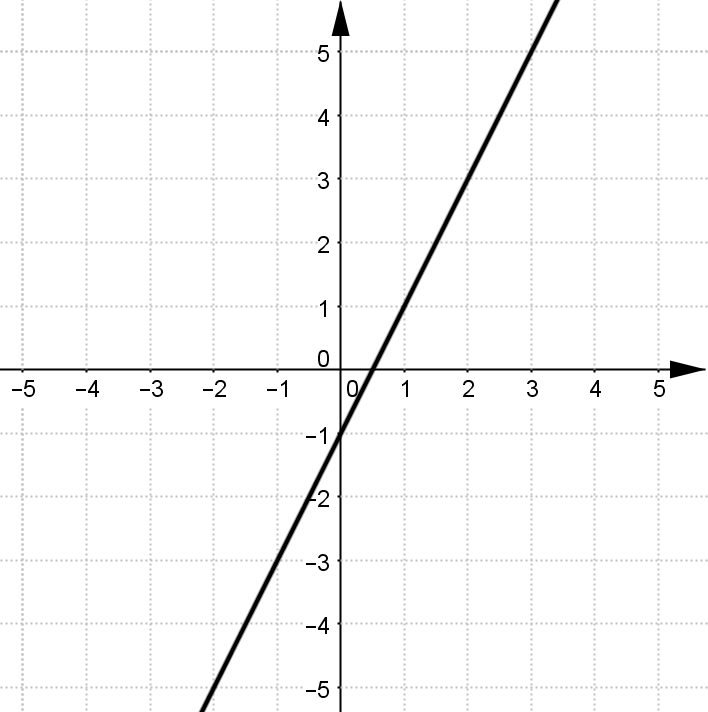
\includegraphics[scale=0.2]{images/51a.png}
	\end{quotation}
	
	\texttt{\tskcol{~~~~~~b) (s.)}}
	\begin{quotation}
		\noindent
		$y=2-x \Leftrightarrow y=-1x+2 \rightarrow$ Lutning: $-1$, korsar y-axeln vid: $2$ \\ \\
		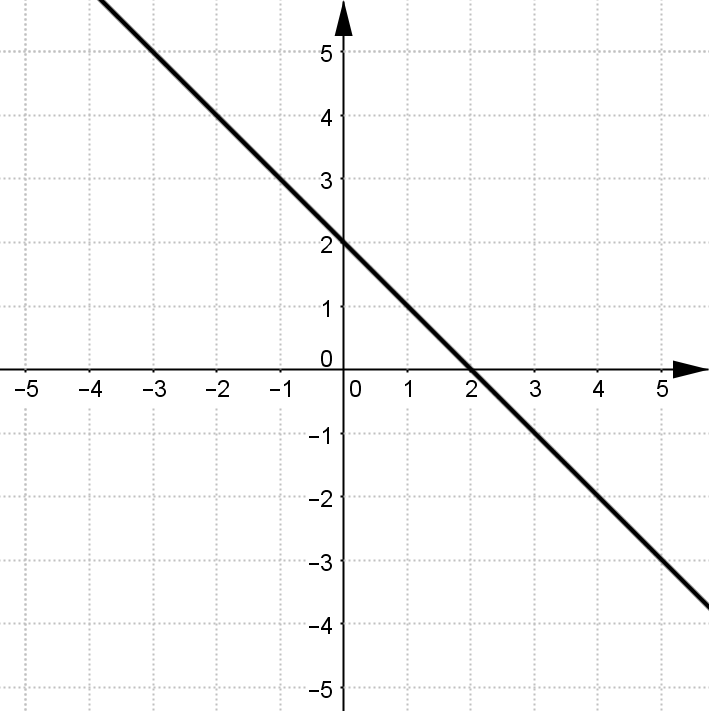
\includegraphics[scale=0.2]{images/51b.png}
	\end{quotation}
	
	\texttt{\tskcol{~~~~~~c) (s.)}}
	\begin{quotation}
		\noindent
		$y=3 \Leftrightarrow y=0x+3 \rightarrow$ Lutning: $0$, korsar y-axeln vid: $3$. Kan också ses som att $y$ är konstant tre oberoende av vad $x$ är. \\ \\
		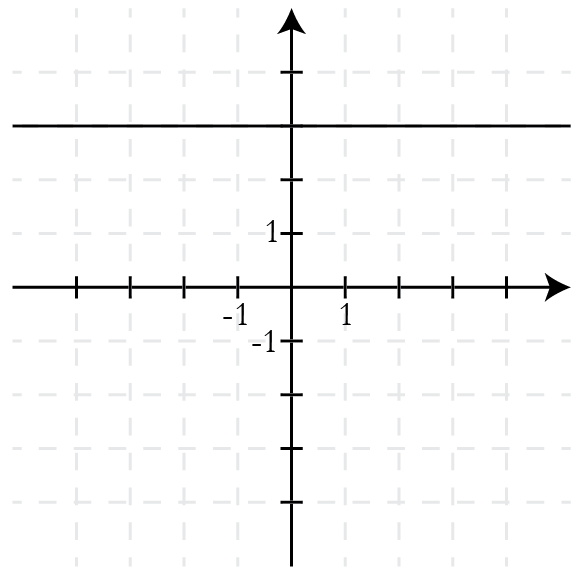
\includegraphics[scale=0.2]{images/51c.png}
	\end{quotation}
	
	\pagebreak
	
	\texttt{\tskcol{~~~~~~d) (s.)}}
	\begin{quotation}
		\noindent
		$x=-2$ kan inte beskrivas med räta linjens ekvation eftersom ekvationen inte är en funktion (saknar värde på $y$ för alla $x$ utom $-2$ och har oändligt många lösningar på $x=-2$). Se det som att för oberoende av vad $y$ är är $x=-2$.  \\ \\
		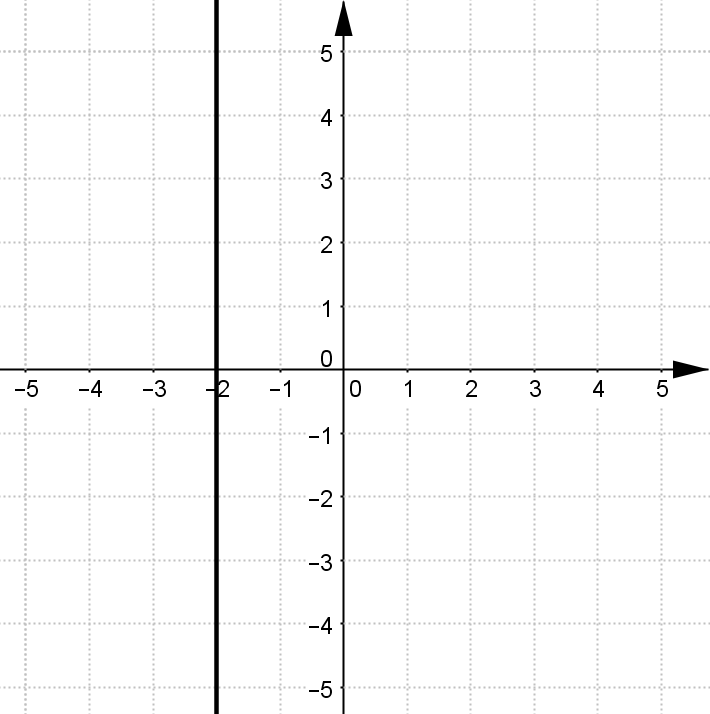
\includegraphics[scale=0.2]{images/51d.png}
	\end{quotation}
	
	\texttt{\tskcol{5.2~~~a) (s.)}}
	\begin{quotation}
		\noindent
		Uppgiften kan lösas på flera sätt, t.ex. med enpunktsformeln eller genom att sätta in värdena i räta linjens ekvation och beräkna $m$.
		\\ \\
		Enpunktsformeln: 
		\[y-2=-1(x-0) \Leftrightarrow 
		y=-x+2\]
		\\
		Räta linjens ekvation:
		\[2=-1*0+m \Leftrightarrow
		m=2\Rightarrow
		y=-x+2\]
		\\
		\textbf{Svar:} $y=-x+2$
	\end{quotation}
	
	\texttt{\tskcol{~~~~~~b) (s.)}}
	\begin{quotation}
		\noindent
		Uppgiften kan lösas på flera sätt, t.ex. med enpunktsformeln eller genom att sätta in värdena i räta linjens ekvation och beräkna $m$.
		\\ \\
		Enpunktsformeln: 
		\[y-1=3(x-2) \Leftrightarrow 
		y=3x-6+1 \Leftrightarrow
		y=3x-5\]
		\\
		Räta linjens ekvation:
		\[1=3*2+m \Leftrightarrow
		m=-5\Rightarrow
		y=3x-5\]
		\\
		\textbf{Svar:} $y=3x-5$
	\end{quotation}
	
	\pagebreak
	\texttt{\tskcol{~~~~~~c) (s.)}}
	\begin{quotation}
		\noindent
		Uppgiften kan lösas på flera sätt, t.ex. med enpunktsformeln eller genom att sätta in värdena i räta linjens ekvation och beräkna $m$.
		\\ \\
		Enpunktsformeln: 
		\[y-b=k(x-a)\]
		\\
		Räta linjens ekvation:
		\[b=ka+m \Leftrightarrow
		m=b-ka
		\]\[
		y=kx-ka+b \Leftrightarrow
		y=k(x-a)+b \Leftrightarrow
		y-b=k(x-a)\]
		\\
		\textbf{Svar:} $y-b=k(x-a)$
	\end{quotation}
	
	\texttt{\tskcol{~~~~~~d) (s.)}}
	\begin{quotation}
		\noindent
		Använd tvåpunktsformeln.
		\[(\overbrace{a}^{x_1},~\overbrace{b}^{y_1})~~~~(\overbrace{a+1}^{x_2},~\overbrace{b+1}^{y_2})\]
		\[y-b=\frac{\cancel{b}+1-\cancel{b}}{\cancel{a}+1-\cancel{a}}(x-a)\Leftrightarrow
		y=1(x-a)+b \Leftrightarrow
		y=x+b-a\]
		\\
		\textbf{Svar:} $y=x+b-a$
	\end{quotation}
	
	\texttt{\tskcol{5.3~~~~~ (s.)}}
	\begin{quotation}
		\noindent
		Använd tvåpunktsformeln med $(-2,5)$ och $(0,-3)$ som punkter ($m$-värdet ger den andra punkten).
		\[y-5=\frac{-3-5}{0+2}(x+2) \Leftrightarrow
		y=-4(x+2)+5 \Leftrightarrow
		y=-4x-3\]
		\\
		\textbf{Svar:} $a=-4$
	\end{quotation}
	
	\texttt{\tskcol{5.4~~~a) (s.)}}
	\begin{quotation}
		\noindent
		Använd tvåpunktsformeln.
		\[y-1=\frac{-2-1}{1+2}(x+2) \Leftrightarrow
		y=\frac{-3}{3}(x+2)+1 \Leftrightarrow
		y=-x-1\]
		\\
		\textbf{Svar:} $y=-x-1$
	\end{quotation}
	
	\texttt{\tskcol{~~~~~~b) (s.)}}
	\begin{quotation}
		\noindent
		Använd tvåpunktsformeln.
		\[y-2=\frac{2-2}{2+1}(x+1) \Leftrightarrow
		y=0(x+1)+2 \Leftrightarrow
		y=2\]
		\\
		\textbf{Svar:} $y=2$
	\end{quotation}
	
	\texttt{\tskcol{~~~~~~c) (s.)}}
	\begin{quotation}
		\noindent
		Använd tvåpunktsformeln.
		\[y-0=\underbrace{\frac{2-0}{1-1}}_\text{ej def.}(x-1)\]
		Att tvåpunktsformeln inte är definierad (nolldivision) innebär att lutningen på linjen är ''oändlig'' vilket i sin tur innebär att det är en vertikal linje. Eftersom båda punkterna ligger på $x=1$ måste det vara ekvationen. 
		\\ \\
		\textbf{Svar:} $x=1$
	\end{quotation}
	
	\texttt{\tskcol{5.5~~~a) (s.)}}
	\begin{quotation}
		\noindent
		Använd tvåpunktsformeln.
		\[y-2=\frac{3-2}{2+1}(x+1) \Leftrightarrow
		y=\frac{1}{3}(x+1)+2 \Leftrightarrow
		y=\frac{1}{3}x+\frac{1}{3}+\frac{6}{3} \Leftrightarrow
		y=\frac{1}{3}x+\frac{7}{3}\]
		Allmän form:
		\[\frac{1}{3}x-y+\frac{7}{3}=0 \Leftrightarrow
		x-3y+7=0\]
		\\
		\textbf{Svar:} $k$-form: $y=\frac{1}{3}x+\frac{7}{3}$ och allmän form: $x-3y+7=0$
	\end{quotation}
	
	\texttt{\tskcol{~~~~~~b) (s.)}}
	\begin{quotation}
		\noindent
		Använd tvåpunktsformeln.
		\[y-3=\frac{3-3}{-7-2}(x-2) \Leftrightarrow
		y=0(x-2)+3 \Leftrightarrow
		y=3\]
		Allmän form:
		\[y-3=0\]
		\\
		\textbf{Svar:} $k$-form: $y=3$ och allmän form: $y-3=0$
	\end{quotation}
	
	\texttt{\tskcol{5.6~~~a) (s.)}}
	\begin{quotation}
		\noindent
		Bestäm först ekvationen för en linje mellan två av punkterna och kolla sedan om den tredje ligger på linjen.
		\\ \\
		Använd tvåpunktsformeln på $(-6,5)$ och $(-2,2)$.
		\begin{align*}
		&y-5=\frac{2-5}{-2+6}(x+6) \Leftrightarrow
		y=\frac{-3}{4}x-\frac{9}{2}+5 \Leftrightarrow
		y=-\frac{3}{4}x+\frac{1}{2} \Leftrightarrow \\ \Leftrightarrow
		&\frac{3}{4}x+y-\frac{1}{2}=0 \Leftrightarrow
		3x+4y-2=0
		\end{align*}
		Testa sedan genom att sätta in värdena för den sista punkten.
		\[3*10+4*(-8)-2=30-32-2=-4\neq0\]
		Punkten ligger alltså inte på linjen.
		\\ \\
		\textbf{Svar:} Nej.
	\end{quotation}
	
	\texttt{\tskcol{~~~~~~b) (s.)}}
	\begin{quotation}
		\noindent
		Bestäm först ekvationen för en linje mellan två av punkterna och kolla sedan om den tredje ligger på linjen.
		\\ \\
		Använd tvåpunktsformeln på $(-7,-5)$ och $(3,1)$.
		\begin{align*}
		&y+5=\frac{1+5}{3+7}(x+7) \Leftrightarrow
		y=\frac{3}{5}(x+7)-5 \Leftrightarrow
		y=\frac{3}{5}x+\frac{21}{5}-\frac{25}{5} \Leftrightarrow \\ \Leftrightarrow
		&\frac{3}{5}x-y-\frac{4}{5}=0 \Leftrightarrow
		3x-5y-4=0
		\end{align*}
		Testa sedan genom att sätta in värdena för den sista punkten.
		\[3*8-5*4-4=24-20-4=0\]
		Punkten ligger alltså på linjen.
		\\ \\
		\textbf{Svar:} Ja
	\end{quotation}
	
	\texttt{\tskcol{5.7~~~a) (s.)}}
	\begin{quotation}
		\noindent
		Lös ekvationssystemet.
		\[\begin{cases} 
		y=2x+1 \\ 
		y=-3x+11
		\end{cases}\]
		Substitutionsmetoden:
		\[2x+1=-3x+11 \Leftrightarrow
		5x=10 \Leftrightarrow
		x=2 \Rightarrow
		y=2*2+1=5\]
		\\
		\textbf{Svar:} punkten $(2,5)$
	\end{quotation}
	
	\texttt{\tskcol{~~~~~~b) (s.)}}
	\begin{quotation}
		\noindent
		Lös ekvationssystemet ($y$-värdet är redan gett i den andra ekvationen).
		\[\begin{cases} 
		y=2x-3 \\ 
		y=5
		\end{cases}\]
		Substitutionsmetoden:
		\[5=2x-3 \Leftrightarrow
		2x=8 \Leftrightarrow
		x=4\]
		\\
		\textbf{Svar:} punkten $(4,5)$
	\end{quotation}
	
	\pagebreak
	\texttt{\tskcol{~~~~~~c) (s.)}}
	\begin{quotation}
		\noindent
		Lös ekvationssystemet ($x$-värdet är redan gett i den andra ekvationen).
		\[\begin{cases} 
		y=3x-2 \\ 
		x=4
		\end{cases}\]
		Substitutionsmetoden:
		\[y=3*4-2 \Leftrightarrow
		y=12-2 \Leftrightarrow
		y=10\]
		\\
		\textbf{Svar:} punkten $(4,10)$
	\end{quotation}
	
	\texttt{\tskcol{~~~~~~d) (s.)}}
	\begin{quotation}
		\noindent
		Lös ekvationssystemet.
		\[\begin{cases} 
		y=5x-4 \\ 
		y=5x+6
		\end{cases}\]
		Substitutionsmetoden:
		\[\cancel{5x}-4=\cancel{5x}+6 \Leftrightarrow
		-4 \neq 6 \Rightarrow \text{Saknar lösning}\]
		\\
		\textbf{Svar:} Skärning saknas
	\end{quotation}
	
	\subsection*{Parabeln}
	
	\texttt{\tskcol{5.8~~~a) (s.)}}
	\begin{quotation}
		\noindent
		\[x^2-3x+2=
		\left(x-\frac{3}{2}\right)^2-\left(\frac{3}{2}\right)^2+2=
		\left(x-\frac{3}{2}\right)^2-\frac{1}{4}\]
		\\ \\
		\textbf{Svar:} $\left(x-\frac{3}{2}\right)^2-\frac{1}{4}$
	\end{quotation}
	
	\texttt{\tskcol{~~~~~~b) (s.)}}
	\begin{quotation}
		\noindent
		Går igenom punkterna $(3/2;-1/4)$ och $(0,2)$. \\
		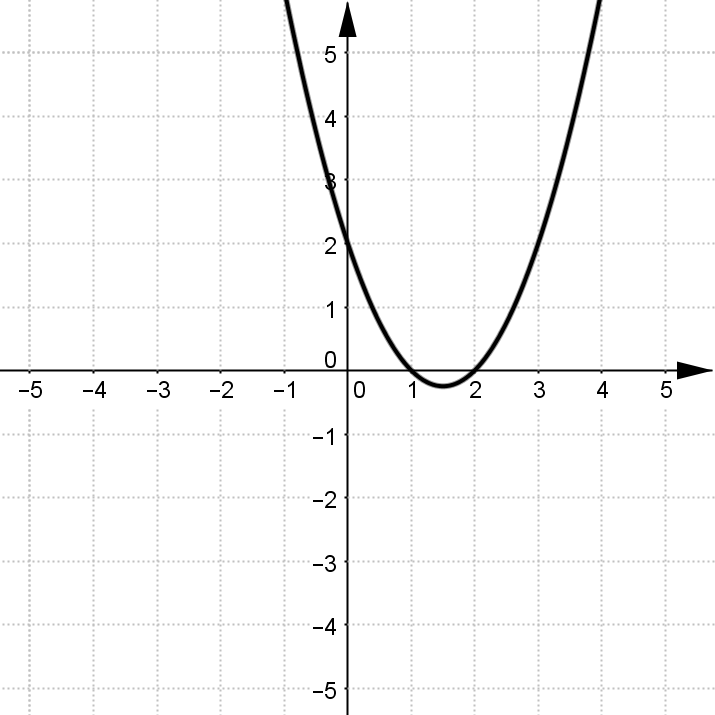
\includegraphics[scale=0.2]{images/58b.png}
	\end{quotation}
	
	\pagebreak
	\texttt{\tskcol{~~~~~~c) (s.)}}
	\begin{quotation}
		\noindent
		$y$ är som minst när $(x-\frac{3}{2})^2$ är så litet som möjligt och eftersom det kvadreras är minsta möjliga värdet 0. Minsta värdet på $y$ är alltså $-\frac{1}{4}$. 
		\\ \\
		\textbf{Svar:} $-\frac{1}{4}$
	\end{quotation}
	
	\texttt{\tskcol{~~~~~~d) (s.)}}
	\begin{quotation}
		\noindent
		Använd pq-formeln.
		\[x^2-3x+2=0 \Leftrightarrow
		x=\frac{3}{2}\pm\sqrt{\left(\frac{3}{2}\right)^2-2}=
		\frac{3}{2}\pm\sqrt{\frac{9-8}{4}}=
		\frac{3}{2}\pm\frac{1}{2}\]
		\[x_1=2,~~x_2=1\]
		\\
		\textbf{Svar:} $x_1=2,~~x_2=1$
	\end{quotation}
	
	\texttt{\tskcol{~~~~~~e) (s.)}}
	\begin{quotation}
		\noindent
		Faktorisera polynomet och använd sedan en teckentabell.
		\[x^2-3x+2 \ge 0 \Leftrightarrow
		(x-2)(x-1) \ge 0\]
		\begin{tabular}{c|c|c|c|c|c}
			$x$                     &     & $1$ &     & $2$ &     \\ \hline
			$x-2$                   & $-$ & $-$ & $-$ & $0$ & $+$ \\
			$x-1$                   & $-$ & $0$ & $+$ & $+$ & $+$ \\ \hline
			$(x-2)(x-1)$  			& $+$ & $0$ & $-$ & $0$ & $+$ \\
		\end{tabular} \\ \\
		När $x \le 0$ eller $x \ge 2$.
		\\ \\
		\textbf{Svar:} $x \le 0$ eller $x \ge 2$
	\end{quotation}
	
	\pagebreak
	\texttt{\tskcol{5.9~~~a) (s.)}}
	\begin{quotation}
		\noindent
		Kvadratkomplettera:
		\[x^2+2x+2=(x+1)^2-1^2+2=(x+1)^2+1\]
		Visualisera: \\
		Går igenom punkterna $(1;1)$ och $(0,2)$. \\
		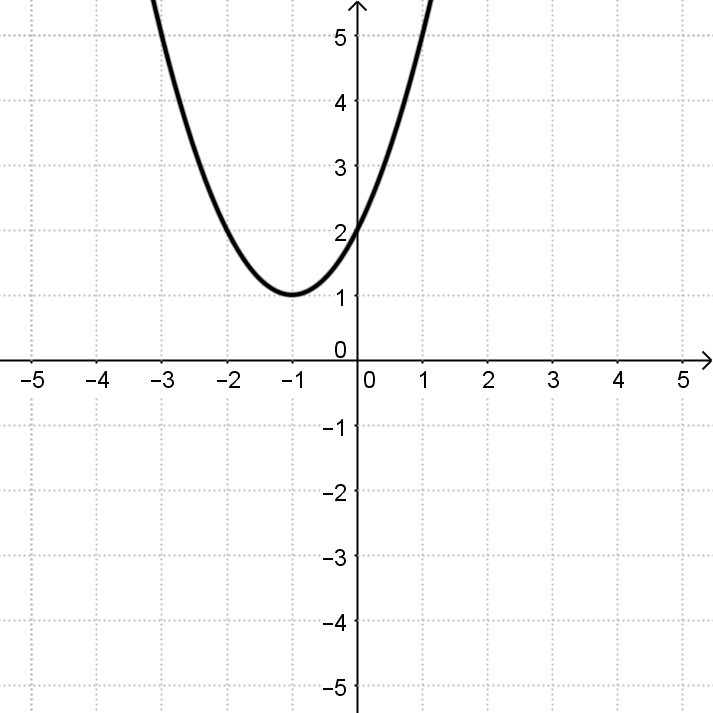
\includegraphics[scale=0.2]{images/59a.png} \\ \\
		Minsta värdet: \\
		Med samma resonemang som i \texttt{\tskcol{5.8 c)}} så är minsta möjliga värdet på $y$ 1. \\ \\
		Lös ekvationen:
		\[x^2+2x+2=0 \Leftrightarrow
		x=-1\pm\sqrt{1^2-2}=-1\pm\sqrt{-1} \Leftarrow 
		\text{Saknar reell lösning}\]
		Lös olikheten:
		\[x^2+2x+2\ge0\]
		Ekvationen saknar nollställen vilket innebär att om någon punkt på linjen är positiv är alla positiva.
		\[0^2+2*0+2=2\]
		Olikheten är alltså sann för alla värden.
	\end{quotation}
	
	\pagebreak
	\texttt{\tskcol{~~~~~~b) (s.)}}
	\begin{quotation}
		\noindent
		Kvadratkomplettera:
		\[x^2-x=(x-\frac{1}{2})^2-(\frac{1}{2})^2=(x-\frac{1}{2})^2-\frac{1}{4}\]
		Visualisera: \\
		Går igenom punkterna $(\frac{1}{2};-\frac{1}{4})$ och $(0,0)$. \\
		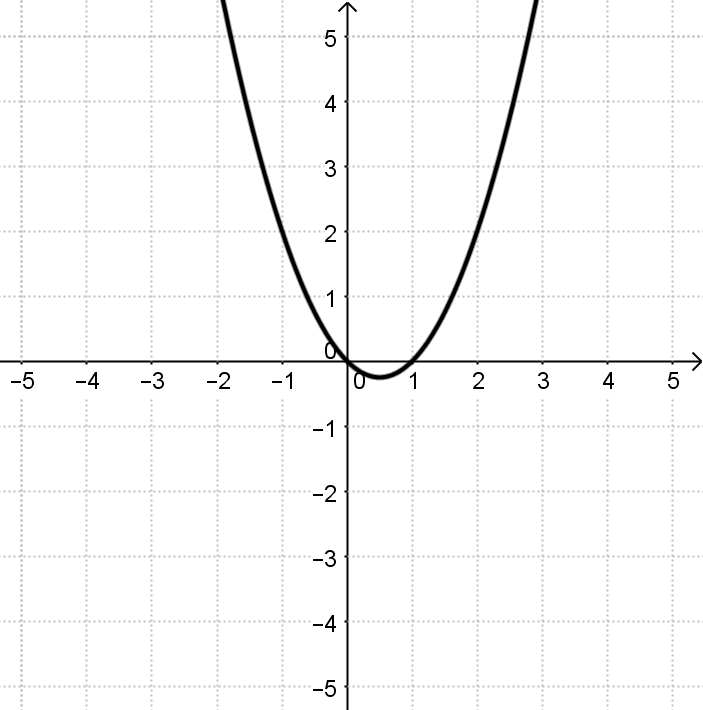
\includegraphics[scale=0.2]{images/59b.png} \\ \\
		Minsta värdet: \\
		Med samma resonemang som i \texttt{\tskcol{5.8 c)}} så är minsta möjliga värdet på $y$ $-\frac{1}{4}$. \\ \\
		Lös ekvationen:
		\[x^2-x=0 \Leftrightarrow
		x=\frac{1}{2}\pm\sqrt{(\frac{1}{2})^2}=\frac{1}{2}\pm\frac{1}{2}\]
		\[x_1=1,~~x_2=0\]
		Lös olikheten:
		\[x^2-x\ge0 \Leftrightarrow
		x(x-1)\ge0\]
		\begin{tabular}{c|c|c|c|c|c}
			$x$                     &     & $0$ &     & $1$ &     \\ \hline
			$x$                     & $-$ & $0$ & $+$ & $+$ & $+$ \\
			$x-1$                   & $-$ & $-$ & $-$ & $0$ & $+$ \\ \hline
			$x(x-1)$  		    	& $+$ & $0$ & $-$ & $0$ & $+$ \\
		\end{tabular} \\ \\
		När $x \le 0$ eller $x \ge 1$.
	\end{quotation}
	
	\pagebreak
	\texttt{\tskcol{~~~~~~c) (s.)}}
	\begin{quotation}
		\noindent
		Kvadratkomplettera:
		\[1-2x-x^2=-(x^2+2x)+1=-((x+1)^2-1^2)+1=-(x+1)^2+1+1=2-(x+1)^2\]
		Visualisera: \\
		Går igenom punkterna $(-1,2)$ och $(0,1)$. \\
		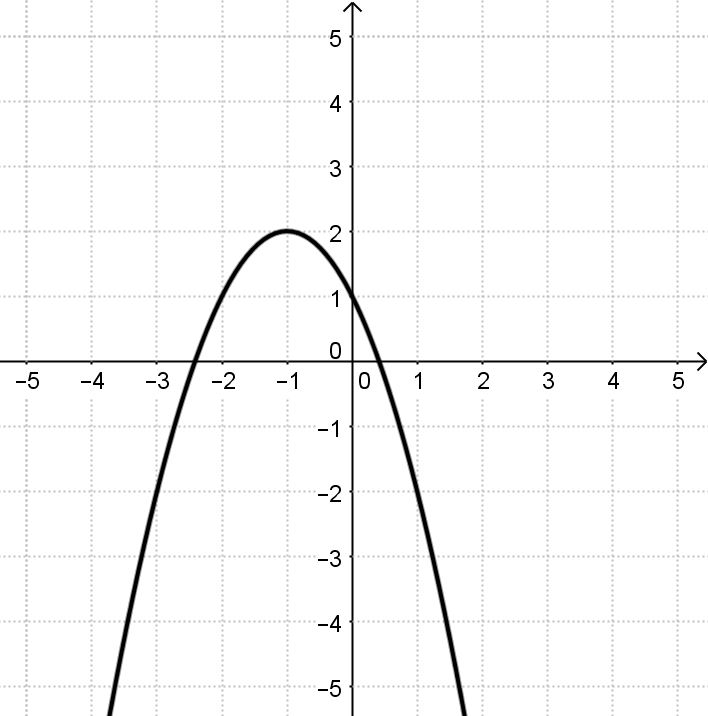
\includegraphics[scale=0.2]{images/59c.png} \\ \\
		Minsta värdet: \\
		Saknar mista värde eftersom när $x$ ökar kommer $y$ bli mindre (pga. negationen). \\ \\
		Lös ekvationen:
		\[1-2x-x^2=0 \Leftrightarrow
		x^2+2x-1=0 \Leftrightarrow
		x=-1\pm\sqrt{1^2+1}=-1\pm\sqrt{2}\]
		\[x=-1\pm\sqrt{2}\]
		Lös olikheten:
		\[1-2x-x^2\ge0 \Leftrightarrow
		-(x^2+2x-1)\ge0 \Leftrightarrow
		-(x+1-\sqrt{2})(x+1+\sqrt{2})\ge0\]
		\begin{tabular}{c|c|c|c|c|c}
			$x$                             &     &$-1-\sqrt{2}$&     &$-1+\sqrt{2}$&     \\ \hline
			$x+1-\sqrt{2}$                  & $-$ &     $-$     & $-$ &     $0$     & $+$ \\
			$x+1+\sqrt{2}$                  & $-$ &     $0$     & $+$ &     $+$     & $+$ \\ 
			$-$                             & $-$ &     $-$     & $-$ &     $-$     & $-$ \\ \hline
			$-(x+1-\sqrt{2})(x+1+\sqrt{2})$	& $-$ &     $0$     & $+$ &     $0$     & $-$ \\
		\end{tabular} \\ \\
		När $-1-\sqrt{2} \le x \le -1+\sqrt{2}$.
	\end{quotation}
	
	\pagebreak
	\texttt{\tskcol{~~~~~~d) (s.)}}
	\begin{quotation}
		\noindent
		Kvadratkomplettera:
		\[2x^2+x+1=2(x^2+\tfrac{1}{2}x)+1=
		2((x+\tfrac{1}{4})^2-(\tfrac{1}{4})^2)+1=
		2(x+\tfrac{1}{4})^2-\tfrac{1}{8}+1=
		2(x+\tfrac{1}{4})^2+\tfrac{7}{8}\]
		Visualisera: \\
		Går igenom punkterna $(-\frac{1}{4},\frac{7}{8})$ och $(0,1)$. \\
		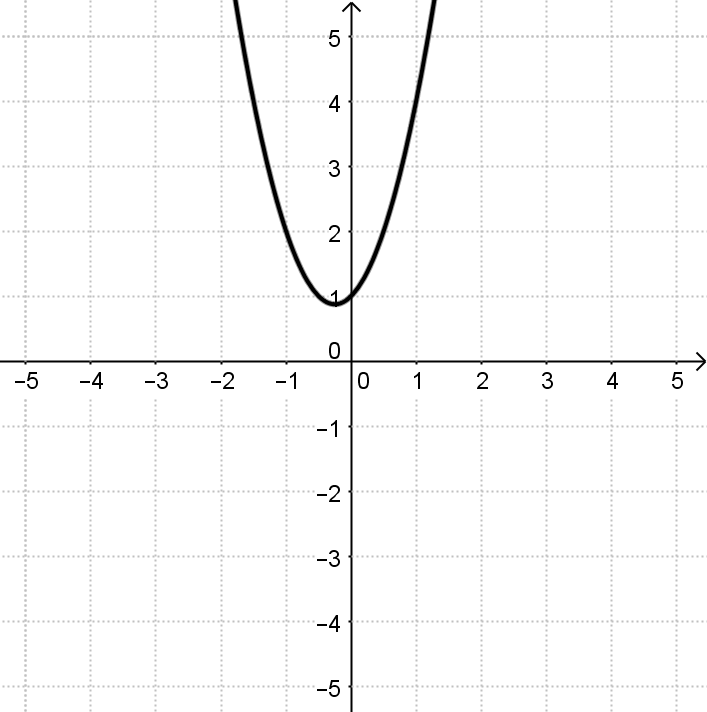
\includegraphics[scale=0.2]{images/59d.png} \\ \\
		Minsta värdet: \\
		Med samma resonemang som i \texttt{\tskcol{5.8 c)}} så är minsta möjliga värdet på $y$ $\frac{7}{8}$. \\ \\
		Lös ekvationen:
		\[2x^2+x+1=0 \Leftrightarrow
		x^2+\frac{1}{2}x+\frac{1}{2}=0 \Leftrightarrow
		x=-\frac{1}{4}\pm\sqrt{(\frac{1}{4})^2-\frac{1}{2}}=-\frac{1}{4}\pm\sqrt{-\frac{7}{16}} \Leftarrow 
		\text{Saknar reell lösning}\]
		Lös olikheten:
		\[2x^2+x+1\ge0\]
		Ekvationen saknar nollställen vilket innebär att om någon punkt på linjen är positiv är alla positiva.
		\[2*0^2+0+1=1\]
		Olikheten är alltså sann för alla värden.
	\end{quotation}
	
	\texttt{\tskcol{5.10~~~~ (s.)}}
	\begin{quotation}
		\noindent
		Kvadratkomplettera:
		\[y-x^2-4x=0 \Leftrightarrow 
		y=x^2+4x=(x+2)^2-2^2=(x+2)^2-4\]
		$y$ är som minst när $(x+2)^2$ är så litet som möjligt och eftersom det kvadreras är minsta möjliga värdet 0. Minsta värdet på $y$ är alltså $-4$. 
		\\ \\
		\textbf{Svar:} $4$
	\end{quotation}
	
	\pagebreak
	\texttt{\tskcol{5.11~~~~ (s.)}}
	\begin{quotation}
		\noindent
		Uppgiften ger ekvationssystemet:
		\[\begin{cases} 
		6=(-1)^2+a*(-1)+b \\ 
		3=2^2+a*2+b
		\end{cases} \Leftrightarrow
		\begin{cases} 
		6=1-a+b \\ 
		3=4+2a+b
		\end{cases} \Leftrightarrow
		\begin{cases} 
		b=a+5 \\ 
		b=-2a-1
		\end{cases}\]
		Substitutionsmetoden:
		\[a+5=-2a-1 \Leftrightarrow
		3a=-6 \Leftrightarrow
		a=-2 ~~~~\Rightarrow
		~~~~b=-2+5=3\]
		\\
		\textbf{Svar:} $a=-2$ och $b=3$
	\end{quotation}
	
	\subsection*{Absolutbelopp}
	
	\texttt{\tskcol{5.12~~a) (s.)}}
	\begin{quotation}
		\noindent
		\[|3|=3\]
		\\
		\textbf{Svar:} $3$
	\end{quotation}
	
	\texttt{\tskcol{~~~~~~b) (s.)}}
	\begin{quotation}
		\noindent
		\[|-3|=3\]
		\\
		\textbf{Svar:} $3$
	\end{quotation}
	
	\texttt{\tskcol{~~~~~~c) (s.)}}
	\begin{quotation}
		\noindent
		\[\sqrt{3^2}=\sqrt{9}=3\]
		\\
		\textbf{Svar:} $3$
	\end{quotation}
	
	\texttt{\tskcol{~~~~~~d) (s.)}}
	\begin{quotation}
		\noindent
		\[\sqrt{(-3)^2}=\sqrt{9}=3\]
		\\
		\textbf{Svar:} $3$
	\end{quotation}
	
	\texttt{\tskcol{~~~~~~e) (s.)}}
	\begin{quotation}
		\noindent
		\[\sqrt{x^2}=x\]
		\\
		\textbf{Svar:} $x$
	\end{quotation}
	
	\pagebreak
	\texttt{\tskcol{~~~~~~f) (s.)}}
	\begin{quotation}
		\noindent
		\[\sqrt{(-x)^2}=x\]
		\\
		\textbf{Svar:} $x$
	\end{quotation}
	
	\texttt{\tskcol{5.13~~a) (s.)}}
	\begin{quotation}
		\noindent
		Använd definitionen av absolutbelopp.
		\[|x|=
		\begin{cases}
		 x& \text{då } x \ge 0 \\
		-x& \text{då } x < 0
		\end{cases}\]
		\begin{align*}
		& x \ge 0:~~ x=4 \\
		& x < 0:~~ -x=4 \Leftrightarrow x=-4
		\end{align*}
		\\
		\textbf{Svar:} $x=4$ eller $x=-4$
	\end{quotation}
	
	\texttt{\tskcol{~~~~~~b) (s.)}}
	\begin{quotation}
		\noindent
		Använd definitionen av absolutbelopp. Andra är en falsk lösning eftersom lösningen inte ligger inom intervallet som $x$ får vara.
		\[|x|=
		\begin{cases}
		x& \text{då } x \ge 0 \\
		-x& \text{då } x < 0
		\end{cases}\]
		\begin{align*}
		& x \ge 0:~~ x=0 \\
		& x < 0:~~ -x=0 \Leftrightarrow x=0\not< 0 \Rightarrow\text{falsk lösning}
		\end{align*}
		\\
		\textbf{Svar:} $x=0$
	\end{quotation}
	
	\texttt{\tskcol{~~~~~~c) (s.)}}
	\begin{quotation}
		\noindent
		Använd definitionen av absolutbelopp. Båda är en falsk lösning eftersom lösningarna inte ligger inom intervallet som $x$ får vara.
		\[|x|=
		\begin{cases}
		x& \text{då } x \ge 0 \\
		-x& \text{då } x < 0
		\end{cases}\]
		\begin{align*}
		& x \ge 0:~~ x=-1 \not\ge 0 \Rightarrow\text{falsk lösning} \\
		& x < 0:~~ -x=-1 \Leftrightarrow x=1 \not< 0 \Rightarrow\text{falsk lösning}
		\end{align*}
		\\
		\textbf{Svar:} ekvationen saknar lösning
	\end{quotation}
	
	\pagebreak
	\texttt{\tskcol{~~~~~~d) (s.)}}
	\begin{quotation}
		\noindent
		Använd definitionen av absolutbelopp.
		\[|x-2|=
		\begin{cases}
		x-2&    \text{då } x-2 \ge 0 \text{ dvs. } x \ge 2\\
		-(x-2)& \text{då } x-2 < 0   \text{ dvs. } x < 2
		\end{cases}\]
		\begin{align*}
		& x \ge 2:~~ x-2=4 \Leftrightarrow x=6 \\
		& x < 2:~~ -(x-2)=4 \Leftrightarrow x=-2
		\end{align*}
		\\
		\textbf{Svar:} $x=6$ eller $x=-2$
	\end{quotation}
	
	\texttt{\tskcol{~~~~~~e) (s.)}}
	\begin{quotation}
		\noindent
		Använd definitionen av absolutbelopp.
		\[|x+4|=
		\begin{cases}
		x+4&    \text{då } x+4 \ge 0 \text{ dvs. } x \ge -4\\
		-(x+4)& \text{då } x+4 < 0   \text{ dvs. } x < -4
		\end{cases}\]
		\begin{align*}
		& x \ge -4:~~ x+4=3 \Leftrightarrow x=-1 \\
		& x < -4:~~ -(x+4)=3 \Leftrightarrow x=-7
		\end{align*}
		\\
		\textbf{Svar:} $x=-1$ eller $x=-7$
	\end{quotation}
	
	\texttt{\tskcol{~~~~~~f) (s.)}}
	\begin{quotation}
		\noindent
		Använd definitionen av absolutbelopp.
		\[|2x+1|=
		\begin{cases}
		2x+1&    \text{då } 2x+1 \ge 0 \text{ dvs. } x \ge -\tfrac{1}{2}\\
		-(2x+1)& \text{då } 2x+1 < 0   \text{ dvs. } x < -\tfrac{1}{2}
		\end{cases}\]
		\begin{align*}
		& x \ge -\tfrac{1}{2}:~~ 2x+1=1 \Leftrightarrow x=0 \\
		& x < -\tfrac{1}{2}:~~ -(2x+1)=1 \Leftrightarrow x=-1
		\end{align*}
		\\
		\textbf{Svar:} $x=0$ eller $x=-1$
	\end{quotation}
	
	\texttt{\tskcol{~~~~~~g) (s.)}}
	\begin{quotation}
		\noindent
		Använd definitionen av absolutbelopp.
		\[|1-x|=
		\begin{cases}
		1-x&    \text{då } 1-x \ge 0 \text{ dvs. } x \le 1\\
		-(1-x)& \text{då } 1-x < 0   \text{ dvs. } x > 1
		\end{cases}\]
		\begin{align*}
		& x \le 1:~~ 1-x=1 \Leftrightarrow x=0 \\
		& x > 1:~~ -(1-x)=1 \Leftrightarrow x=2
		\end{align*}
		\\
		\textbf{Svar:} $x=0$ eller $x=2$
	\end{quotation}
	
	\texttt{\tskcol{5.14~~a) (s.)}}
	\begin{quotation}
		\noindent
		Definitionen av kvadratroten:
		\[\text{Om } a^2 = b \text{ och } a \ge 0 \text{ då är } a = \sqrt{b}\]
		Vilket innebär att $\sqrt{a^2} = a$ om $a \ge 0$. \\ \\
		Använd nu faktumet att $|a|$ alltid är positivt och regeln $a^2=|a|^2$.
		\[\sqrt{x^2}=\sqrt{|x|^2}=|x| \text{ V.S.V}\]
	\end{quotation}
	
	\texttt{\tskcol{~~~~~~b) (s.)}}
	\begin{quotation}
		\noindent
		Använd definitionen av absolutbelopp och att $\sqrt{x^2}=|x|$.
		\[\sqrt{(x-1)^2}=
		|x-1|=
		\begin{cases}
		x-1&    \text{då } x-1 \ge 0 \text{ dvs. } x \ge 1\\
		-(x-1)& \text{då } x-1 < 0   \text{ dvs. } x < 1
		\end{cases}\]
		\begin{align*}
		& x \le 1:~~ x-1=3 \Leftrightarrow x=4 \\
		& x > 1:~~ -(x-1)=3 \Leftrightarrow x=-2
		\end{align*}
		\\
		\textbf{Svar:} $x=4$ eller $x=-2$
	\end{quotation}
	
	\texttt{\tskcol{5.15~~a) (s.)}}
	\begin{quotation}
		\noindent
		Använd definitionen av absolutbelopp.
		\[|x|=
		\begin{cases}
		x& \text{då } x \ge 0 \\
		-x& \text{då } x < 0
		\end{cases}\]
		\begin{align*}
		& x \ge 0:~~ x=3 \\
		& x < 0:~~ -x=3 \Leftrightarrow x=-3
		\end{align*}
		\\
		\textbf{Svar:} $x=3$ eller $x=-3$
	\end{quotation}
	
	\texttt{\tskcol{~~~~~~b) (s.)}}
	\begin{quotation}
		\noindent
		Använd definitionen av absolutbelopp.
		\[|x|=
		\begin{cases}
		x& \text{då } x \ge 0 \\
		-x& \text{då } x < 0
		\end{cases}\]
		\begin{align*}
		& x \ge 0:~~ x<3 \\
		& x < 0:~~ -x<3 \Leftrightarrow x>-3
		\end{align*}
		Kombinera sedan definitionsmängden för uttrycket och uttrycket.
		\[-3 < x < 0 \text{ eller } 0 \le x < 3 \Leftrightarrow -3 < x < 3\]
		\\
		\textbf{Svar:} $-3 < x < 3$
	\end{quotation}
	
	\texttt{\tskcol{~~~~~~c) (s.)}}
	\begin{quotation}
		\noindent
		Använd definitionen av absolutbelopp.
		\[|x|=
		\begin{cases}
		x& \text{då } x \ge 0 \\
		-x& \text{då } x < 0
		\end{cases}\]
		\begin{align*}
		& x \ge 0:~~ x \ge 3 \\
		& x < 0:~~ -x \ge 3 \Leftrightarrow x \le -3
		\end{align*}
		Kombinera sedan definitionsmängden för uttrycket och uttrycket.
		\[x \ge 3 \text{ eller } x \le -3\]
		\\
		\textbf{Svar:} $x \ge 3$ eller $x \le -3$
	\end{quotation}
	
	\texttt{\tskcol{~~~~~~d) (s.)}}
	\begin{quotation}
		\noindent
		Använd definitionen av absolutbelopp.
		\[|x-1|=
		\begin{cases}
		x-1&    \text{då } x-1 \ge 0 \text{ dvs. } x \ge 1\\
		-(x-1)& \text{då } x-1 < 0   \text{ dvs. } x < 1
		\end{cases}\]
		\begin{align*}
		& x \le 1:~~ x-1=3 \Leftrightarrow x=4 \\
		& x > 1:~~ -(x-1)=3 \Leftrightarrow x=-2
		\end{align*}
		\\
		\textbf{Svar:} $x=4$ eller $x=-2$
	\end{quotation}
	
	\texttt{\tskcol{~~~~~~e) (s.)}}
	\begin{quotation}
		\noindent
		Använd definitionen av absolutbelopp.
		\[|x-1|=
		\begin{cases}
		x-1&    \text{då } x-1 \ge 0 \text{ dvs. } x \ge 1\\
		-(x-1)& \text{då } x-1 < 0   \text{ dvs. } x < 1
		\end{cases}\]
		\begin{align*}
		& x \ge 1:~~ x-1 < 3 \Leftrightarrow x < 4\\
		& x < 1:~~ -(x-1) < 3 \Leftrightarrow x > -2
		\end{align*}
		Kombinera sedan definitionsmängden för uttrycket och uttrycket.
		\[-2 < x < 1 \text{ eller } 1 \le x < 4 \Leftrightarrow -2 < x < 4\]
		\\
		\textbf{Svar:} $-2 < x < 4$
	\end{quotation}
	
	\pagebreak
	\texttt{\tskcol{~~~~~~f) (s.)}}
	\begin{quotation}
		\noindent
		Använd definitionen av absolutbelopp.
		\[|x-1|=
		\begin{cases}
		x-1&    \text{då } x-1 \ge 0 \text{ dvs. } x \ge 1\\
		-(x-1)& \text{då } x-1 < 0   \text{ dvs. } x < 1
		\end{cases}\]
		\begin{align*}
		& x \ge 1:~~ x-1 \ge 3 \Leftrightarrow x \ge 4\\
		& x < 1:~~ -(x-1) \ge 3 \Leftrightarrow x \le -2
		\end{align*}
		Kombinera sedan definitionsmängden för uttrycket och uttrycket.
		\[x \ge 4 \text{ eller } x \le -2\]
		\\
		\textbf{Svar:} $x \ge 4$ eller $x \le -2$
	\end{quotation}
	
	\texttt{\tskcol{5.16~~a) (s.)}}
	\begin{quotation}
		\noindent
		Använd definitionen av absolutbelopp.
		\[|x|=
		\begin{cases}
		x& \text{då } x \ge 0 \\
		-x& \text{då } x < 0
		\end{cases}\]
		\begin{align*}
		& x \ge 0:~~ x \le 1 \\
		& x < 0:~~ -x \le 1 \Leftrightarrow x \ge -1
		\end{align*}
		Kombinera sedan definitionsmängden för uttrycket och uttrycket.
		\[-1 \le x < 0 \text{ eller } 0 \le x \le 1 \Leftrightarrow -1 \le x \le 1\]
		$-1 \le x \le 1$ \\ \\
		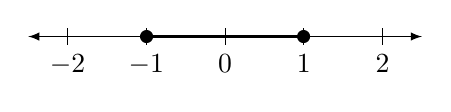
\begin{tikzpicture}
		\draw[latex-latex] (-2.5,0) -- (2.5,0) ; %edit here for the axis
		\foreach \x in  {-2,-1,0,1,2} % edit here for the vertical lines
		\draw[shift={(\x,0)},color=black] (0pt,3pt) -- (0pt,-3pt);
		\foreach \x in {-2,-1,0,1,2} % edit here for the numbers
		\draw[shift={(\x,0)},color=black] (0pt,0pt) -- (0pt,-3pt) node[below] 
		{$\x$};
		\draw[*-*] (-1.08,0) -- (1.08,0);
		\draw[very thick] (-1.08,0) -- (0.92,0);
		\end{tikzpicture}
	\end{quotation}
	
	\texttt{\tskcol{~~~~~~b) (s.)}}
	\begin{quotation}
		\noindent
		Använd definitionen av absolutbelopp.
		\[|x|=
		\begin{cases}
		x& \text{då } x \ge 0 \\
		-x& \text{då } x < 0
		\end{cases}\]
		\begin{align*}
		& x \ge 0:~~ x \ge 2 \\
		& x < 0:~~ -x \ge 2 \Leftrightarrow x \le -2
		\end{align*}
		Kombinera sedan definitionsmängden för uttrycket och uttrycket. \\ \\
		$x \le -2$ eller $x \ge 2$\\ \\
		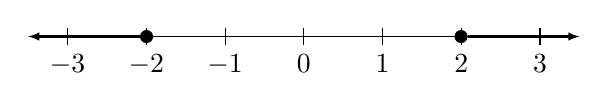
\begin{tikzpicture}
		\draw[latex-latex] (-3.5,0) -- (3.5,0) ; %edit here for the axis
		\foreach \x in  {-3,-2,-1,0,1,2,3} % edit here for the vertical lines
		\draw[shift={(\x,0)},color=black] (0pt,3pt) -- (0pt,-3pt);
		\foreach \x in {-3,-2,-1,0,1,2,3} % edit here for the numbers
		\draw[shift={(\x,0)},color=black] (0pt,0pt) -- (0pt,-3pt) node[below] 
		{$\x$};
		\draw[*-*] (-2.08,0) -- (2.08,0);
		\draw[very thick] (-3.4,0) -- (-2.08,0);
		\draw[very thick] (2.08,0) -- (3.4,0);
		\end{tikzpicture}
	\end{quotation}
	
	\texttt{\tskcol{~~~~~~c) (s.)}}
	\begin{quotation}
		\noindent
		Använd definitionen av absolutbelopp.
		\[|x-1|=
		\begin{cases}
		x-1&    \text{då } x-1 \ge 0 \text{ dvs. } x \ge 1\\
		-(x-1)& \text{då } x-1 < 0   \text{ dvs. } x < 1
		\end{cases}\]
		\begin{align*}
		& x \ge 1:~~ x-1 < 2 \Leftrightarrow x < 3\\
		& x < 1:~~ -(x-1) < 2 \Leftrightarrow x > -1
		\end{align*}
		Kombinera sedan definitionsmängden för uttrycket och uttrycket.
		\[-1 < x < 1 \text{ eller } 1 \le x < 3 \Leftrightarrow -1 < x < 3\]
		$-1 < x < 3$ \\ \\
		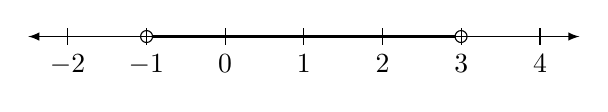
\begin{tikzpicture}
		\draw[latex-latex] (-2.5,0) -- (4.5,0) ; %edit here for the axis
		\foreach \x in  {-2,-1,0,1,2,3,4} % edit here for the vertical lines
		\draw[shift={(\x,0)},color=black] (0pt,3pt) -- (0pt,-3pt);
		\foreach \x in {-2,-1,0,1,2,3,4} % edit here for the numbers
		\draw[shift={(\x,0)},color=black] (0pt,0pt) -- (0pt,-3pt) node[below] 
		{$\x$};
		\draw[o-o] (-1.08,0) -- (3.08,0);
		\draw[very thick] (-0.92,0) -- (2.92,0);
		\end{tikzpicture}
	\end{quotation}
	
	\texttt{\tskcol{~~~~~~d) (s.)}}
	\begin{quotation}
		\noindent
		Använd definitionen av absolutbelopp.
		\[|x+2|=
		\begin{cases}
		x+2&    \text{då } x+2 \ge 0 \text{ dvs. } x \ge -2\\
		-(x+2)& \text{då } x+2 < 0   \text{ dvs. } x < -2
		\end{cases}\]
		\begin{align*}
		& x \ge -2:~~ x+2 < 1 \Leftrightarrow x < -1\\
		& x < -2:~~ -(x+2) < 1 \Leftrightarrow x > -3
		\end{align*}
		Kombinera sedan definitionsmängden för uttrycket och uttrycket.
		\[-3 < x < -2 \text{ eller } -2 \le x < -1 \Leftrightarrow -3 < x < -1\]
		$-3 < x < -1$ \\ \\
		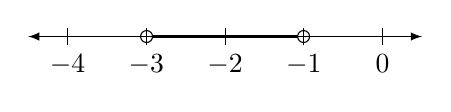
\begin{tikzpicture}
		\draw[latex-latex] (-4.5,0) -- (0.5,0) ; %edit here for the axis
		\foreach \x in  {-4,-3,-2,-1,0} % edit here for the vertical lines
		\draw[shift={(\x,0)},color=black] (0pt,3pt) -- (0pt,-3pt);
		\foreach \x in {-4,-3,-2,-1,0} % edit here for the numbers
		\draw[shift={(\x,0)},color=black] (0pt,0pt) -- (0pt,-3pt) node[below] 
		{$\x$};
		\draw[o-o] (-3.08,0) -- (-0.92,0);
		\draw[very thick] (-2.92,0) -- (-1.08,0);
		\end{tikzpicture}
		\\ \\
		\textbf{Svar:}
	\end{quotation}
	
	\texttt{\tskcol{5.17~~a) (s.)}}
	\begin{quotation}
		\noindent
		Använd definitionen av absolutbelopp.
		\[|x-3|=
		\begin{cases}
		x-3&    \text{då } x-3 \ge 0 \text{ dvs. } x \ge 3\\
		-(x-3)& \text{då } x-3 < 0   \text{ dvs. } x < 3
		\end{cases}\]
		\begin{align*}
		& x \ge 3:~~ x-3 = 1-2x \Leftrightarrow x = \frac{4}{3} \not\ge 3 \Rightarrow\text{falsk lösning}\\
		& x < 3:~~ -(x-3) = 1-2x \Leftrightarrow x = -2
		\end{align*}
		\\ 
		\textbf{Svar:} $x=-2$
	\end{quotation}
	
	\texttt{\tskcol{~~~~~~b) (s.)}}
	\begin{quotation}
		\noindent
		Använd definitionen av absolutbelopp.
		\[|x-2|=
		\begin{cases}
		x-2&    \text{då } x-2 \ge 0 \text{ dvs. } x \ge 2\\
		-(x-2)& \text{då } x-2 < 0   \text{ dvs. } x < 2
		\end{cases}\]
		\begin{align*}
		& x \ge 2:~~ x-2 = x+1 \Leftrightarrow -2 \neq 1 \Rightarrow\text{ingen lösning}\\
		& x < 2:~~ -(x-2) = x+1 \Leftrightarrow x = \frac{1}{2}
		\end{align*}
		\\ 
		\textbf{Svar:} $x=\frac{1}{2}$
	\end{quotation}
	
	\texttt{\tskcol{~~~~~~c) (s.)}}
	\begin{quotation}
		\noindent
		Använd definitionen av absolutbelopp.
		\[|2x+1|=
		\begin{cases}
		2x+1&    \text{då } 2x+1 \ge 0 \text{ dvs. } x \ge -\frac{1}{2}\\
		-(2x+1)& \text{då } 2x+1 < 0   \text{ dvs. } x < -\frac{1}{2}
		\end{cases}\]
		\begin{align*}
		& x \ge -\frac{1}{2}:~~ 2x+1 = x-1 \Leftrightarrow x = -2 \not\ge -\frac{1}{2} \Rightarrow\text{falsk lösning}\\
		& x < -\frac{1}{2}:~~ -(2x+1) = x-1 \Leftrightarrow x = 0 \not< -\frac{1}{2} \Rightarrow\text{falsk lösning}	
		\end{align*}
		\\ 
		\textbf{Svar:} Saknar lösning
	\end{quotation}
	
	\texttt{\tskcol{5.18~~a) (s.)}}
	\begin{quotation}
		\noindent
		Använd definitionen av absolutbelopp.
		\[|x|=
		\begin{cases}
		x& \text{då } x \ge 0 \\
		-x& \text{då } x < 0
		\end{cases}\]
		\begin{align*}
		& x \ge 0:~~ x-x = 2 \Leftrightarrow 0 \neq 2 \Rightarrow\text{ingen lösning}\\
		& x < 0:~~ -x-x = 2 \Leftrightarrow x = -1
		\end{align*}
		\\ 
		\textbf{Svar:} $x=-1$
	\end{quotation}
	
	\texttt{\tskcol{~~~~~~b) (s.)}}
	\begin{quotation}
		\noindent
		Använd definitionen av absolutbelopp.
		\[|x|=
		\begin{cases}
		x& \text{då } x \ge 0 \\
		-x& \text{då } x < 0
		\end{cases}\]
		\begin{align*}
		& x \ge 0:~~ x^2+2x-3 = 0 \Leftrightarrow 
		\begin{cases}
		x_1=-3\not\ge 0 \Rightarrow\text{falsk lösning} \\
		x_2=1
		\end{cases}\\
		& x < 0:~~ x^2+2(-x)-3 = 0 \Leftrightarrow 
		\begin{cases}
		x_1=3\not< 0 \Rightarrow\text{falsk lösning} \\
		x_2=-1
		\end{cases}
		\end{align*}
		\\ 
		\textbf{Svar:} $x=-1$ eller $x=1$
	\end{quotation}
	
	\texttt{\tskcol{~~~~~~c) (s.)}}
	\begin{quotation}
		\noindent
		Använd definitionen av absolutbelopp.
		\[|x+1|=
		\begin{cases}
		x+1&    \text{då } x+1 \ge 0 \text{ dvs. } x \ge -1\\
		-(x+1)& \text{då } x+1 < 0   \text{ dvs. } x < -1
		\end{cases}\]
		\begin{align*}
		& x \ge -1:~~ x^2+2(x+1)-1 = 0 \Leftrightarrow x^2+2x+1=0 \Leftrightarrow x=-1\\
		& x < -1:~~ x^2+2(-x-1)-1 = 0 \Leftrightarrow x^2-2x-3 = 0 \Leftrightarrow
		\begin{cases}
		x_1=3\not< -1 \Rightarrow\text{falsk lösning} \\
		x_2=-1
		\end{cases}
		\end{align*}
		\\
		\textbf{Svar:} $x=-1$
	\end{quotation}
	
	\texttt{\tskcol{5.19~~a) (s.)}}
	\begin{quotation}
		\noindent
		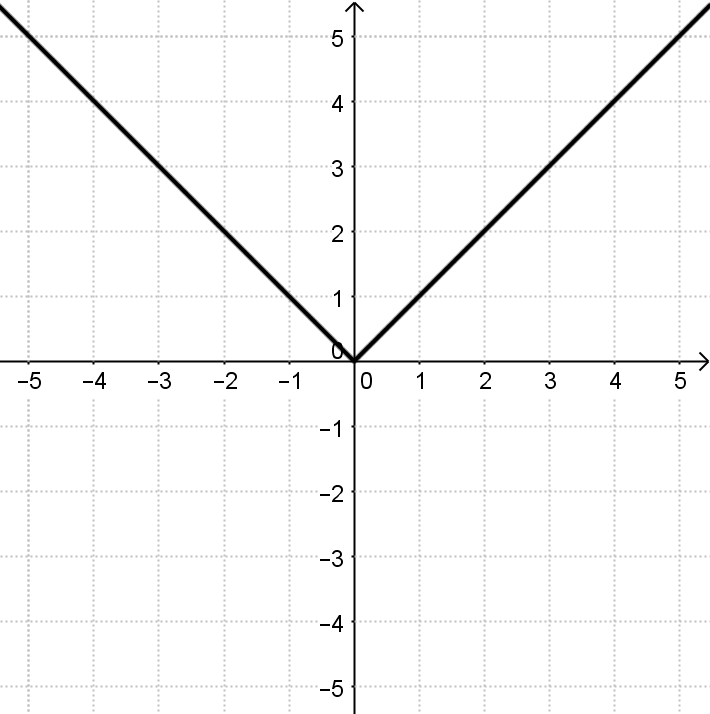
\includegraphics[scale=0.2]{images/519a.png}
	\end{quotation}
	
	\texttt{\tskcol{~~~~~~b) (s.)}}
	\begin{quotation}
		\noindent
		Förskjuten ett steg till höger. \\
		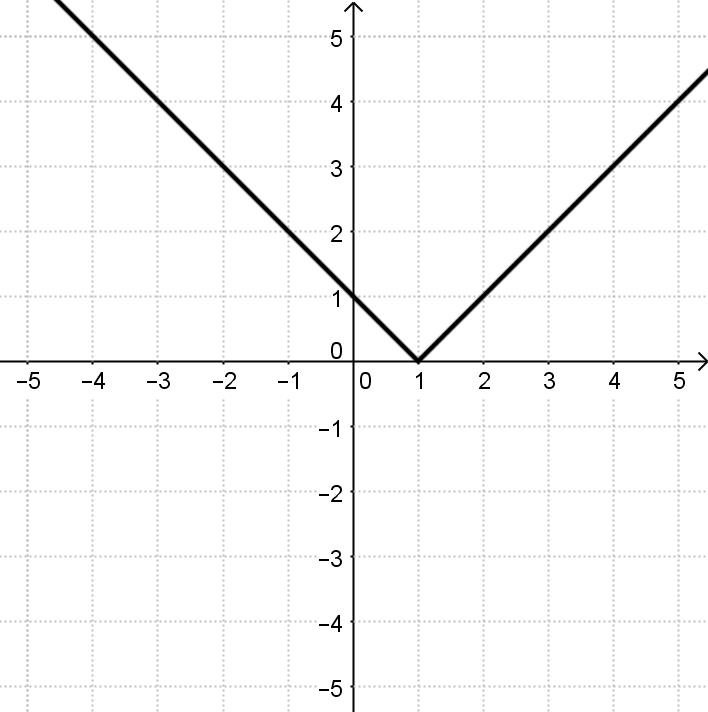
\includegraphics[scale=0.2]{images/519b.png}
	\end{quotation}
	
	\texttt{\tskcol{~~~~~~c) (s.)}}
	\begin{quotation}
		\noindent
		Förskjuten två steg till vänster. \\
		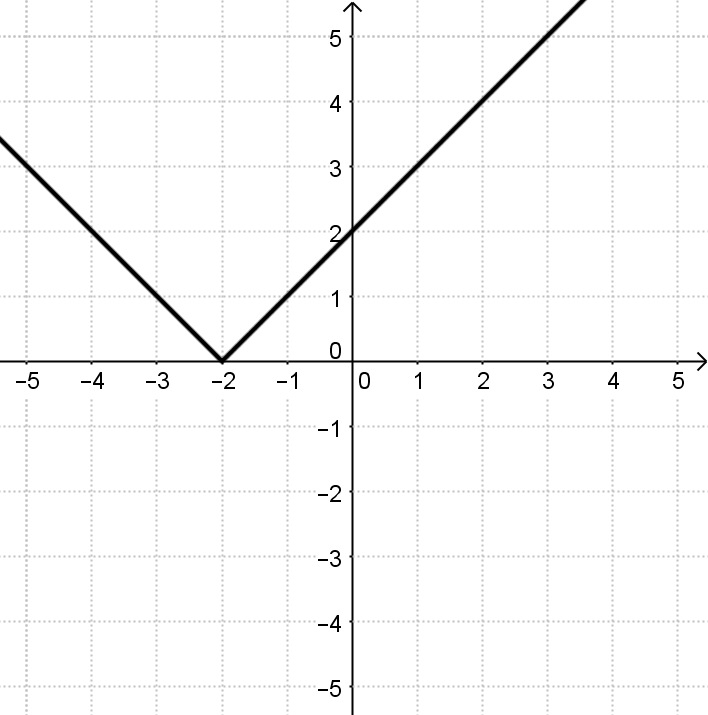
\includegraphics[scale=0.2]{images/519c.png}
	\end{quotation}
	
	\texttt{\tskcol{5.20~~a) (s.)}}
	\begin{quotation}
		\noindent
		När $x$ är större än 2 är det $y=x-2-2x=-x-2$ som gäller och när $x$ är mindre än 2 är det $y=-(x-2)-2x=-3x+2$. \\
		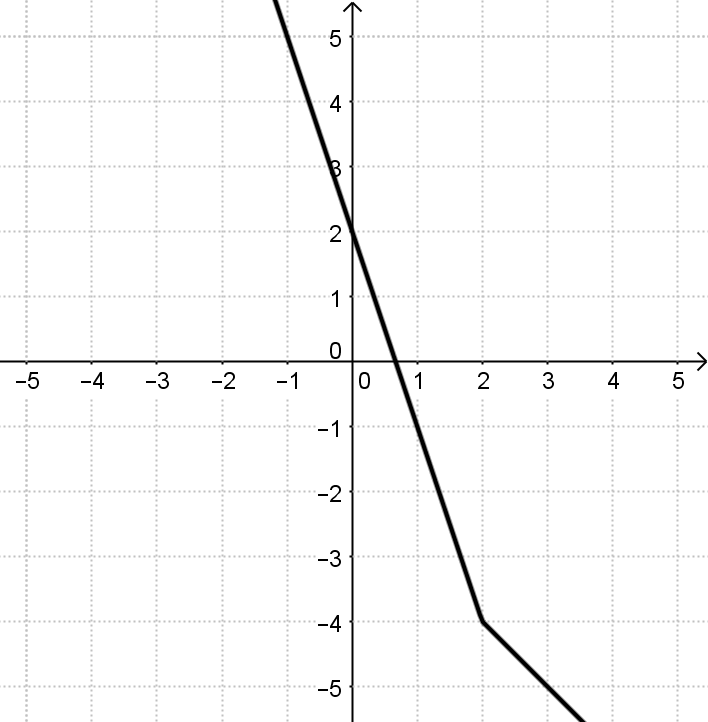
\includegraphics[scale=0.2]{images/520a.png}
	\end{quotation}
	
	\texttt{\tskcol{~~~~~~b) (s.)}}
	\begin{quotation}
		\noindent
		När $x$ är större än 0 så är det $y=x+x=2x$ som gäller och när $x$ är mindre än 0 är det $y=-x+x=0$. \\
		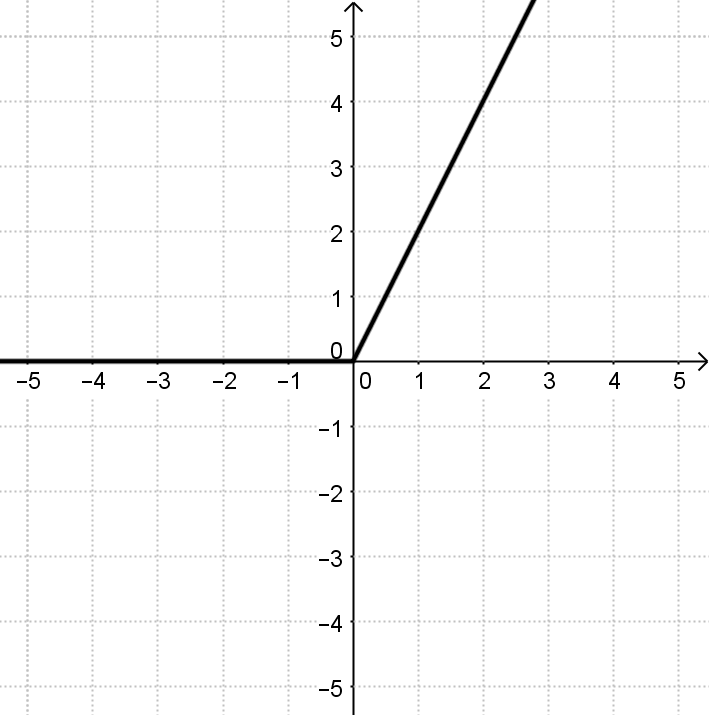
\includegraphics[scale=0.2]{images/520b.png}
	\end{quotation}
	
	\texttt{\tskcol{~~~~~~c) (s.)}}
	\begin{quotation}
		\noindent
		När $x$ är större än 1 så är det $y=x-1+x=2x-1$ som gäller och när $x$ är mindre än 1 är det $y=-(x-1)+x=1$. \\
		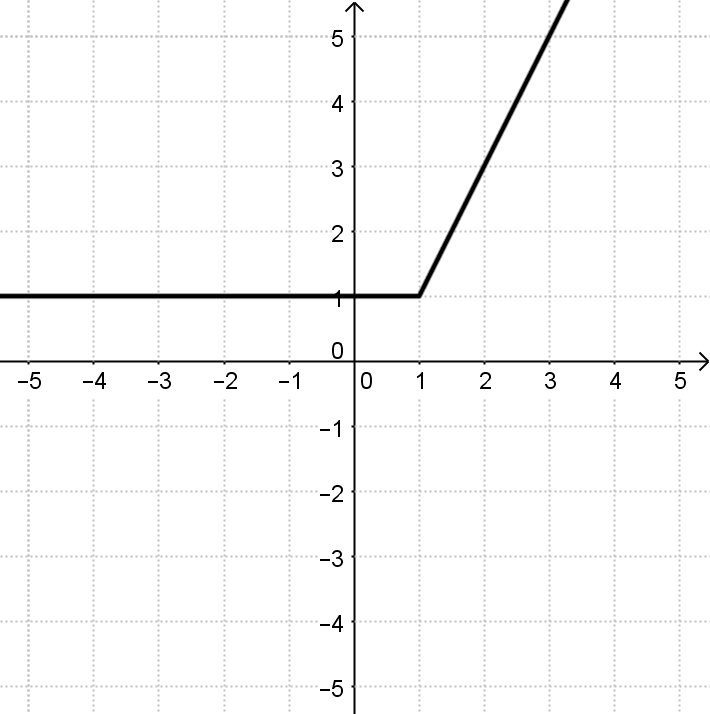
\includegraphics[scale=0.2]{images/520c.png}
	\end{quotation}
	
	\pagebreak
	\texttt{\tskcol{5.21~~~~ (s.)}}
	\begin{quotation}
		\noindent
		Använd definitionen av absolutbelopp (hoppat över ett steg för att det ska vara mer lättläst).
		\[|x+1|=
		\begin{cases}
		x+1&    \text{då } x \ge -1\\
		-(x+1)& \text{då } x < -1
		\end{cases}~~~~~~
		|x-1|=
		\begin{cases}
		x-1&    \text{då } x \ge 1\\
		-(x-1)& \text{då } x < 1
		\end{cases}\]
		Slå samman båda till ett gemensamt uttryck.
		\[|x+1|+|x-1|=
		\begin{cases}
		x+1+x-1&    \text{då } x \ge 1\\
		x+1-(x-1)& \text{då } -1 \le x < 1 \\
		-(x+1)-(x-1)& \text{då } x < -1 
		\end{cases}\]
		\begin{align*}
		     x \ge 1:&~~ x+1+x-1 = 4 \Leftrightarrow 2x=4 \Leftrightarrow x=2\\
		-1 \le x < 1:&~~ x+1-(x-1) = 4 \Leftrightarrow 2 \neq 4 \Rightarrow \text{ ingen lösning}\\
		      x < -1:&~~ -(x+1)-(x-1) = 4 \Leftrightarrow -2x = 4 \Leftrightarrow x = -2
		\end{align*}
		\\
		\textbf{Svar:} $x=2$ eller $x=-2$
	\end{quotation}
	
	\texttt{\tskcol{5.22~~a) (s.)}}
	\begin{quotation}
		\noindent
		Använd definitionen av absolutbelopp (hoppat över ett steg för att det ska vara mer lättläst).
		\[|x+1|=
		\begin{cases}
		x+1&    \text{då } x \ge -1\\
		-(x+1)& \text{då } x < -1
		\end{cases}~~~~~~
		|x-1|=
		\begin{cases}
		x-1&    \text{då } x \ge 1\\
		-(x-1)& \text{då } x < 1
		\end{cases}\]
		Slå samman båda till ett gemensamt uttryck.
		\[|x+1|-|x-1|=
		\begin{cases}
		x+1-(x-1)&    \text{då } x \ge 1\\
		x+1+(x-1)& \text{då } -1 \le x < 1 \\
		-(x+1)+(x-1)& \text{då } x < -1 
		\end{cases}\]
		\begin{align*}
		     x \ge 1:&~~ x+1-(x-1) = 1 \Leftrightarrow 2 \neq 1 \Rightarrow \text{ ingen lösning}\\
		-1 \le x < 1:&~~ x+1+(x-1) = 1 \Leftrightarrow 2x = 1 \Leftrightarrow x = \frac{1}{2}\\
		      x < -1:&~~ -(x+1)+(x-1) = 1 \Leftrightarrow -2 \neq 1 \Rightarrow \text{ ingen lösning}
		\end{align*}
		\\
		\textbf{Svar:} $x = \frac{1}{2}$
	\end{quotation}
	
	\texttt{\tskcol{~~~~~~b) (s.)}}
	\begin{quotation}
		\noindent
		Använd resonemanget från uppgift \texttt{\tskcol{a)}} för intervallen.
		\begin{align*}
		     x \ge 1:&~~ x+1-(x-1) = 3 \Leftrightarrow 2 \neq 3 \Rightarrow \text{ ingen lösning}\\
		-1 \le x < 1:&~~ x+1+(x-1) = 3 \Leftrightarrow 2x = 3 \Leftrightarrow x = \frac{3}{2} \not< 1 \Rightarrow\text{falsk lösning}\\
		      x < -1:&~~ -(x+1)+(x-1) = 3 \Leftrightarrow -2 \neq 3 \Rightarrow \text{ ingen lösning}
		\end{align*}
		\\
		\textbf{Svar:} saknar lösning
	\end{quotation}
	
	\texttt{\tskcol{~~~~~~c) (s.)}}
	\begin{quotation}
		\noindent
		Använd resonemanget från uppgift \texttt{\tskcol{a)}} för intervallen.
		\begin{align*}
		x \ge 1:&~~ x+1-(x-1) = -2 \Leftrightarrow 2 \neq -2 \Rightarrow \text{ ingen lösning}\\
		-1 \le x < 1:&~~ x+1+(x-1) = -2 \Leftrightarrow 2x = -2 \Leftrightarrow x = -1\\
		x < -1:&~~ -(x+1)+(x-1) = -2 \Leftrightarrow -2 = -2 \Rightarrow \text{ alla lösningar}
		\end{align*}
		\[x < -1 \text{ eller } x=-1 \Leftrightarrow x \le -1\]
		\\
		\textbf{Svar:} $x \le -1$
	\end{quotation}
	
	\texttt{\tskcol{~~~~~~d) (s.)}}
	\begin{quotation}
		\noindent
		Under $-2$ är $y=-2$, mellan $-2$ och $2$ är $y=2x$ och efter $2$ är $y=2$. \\
		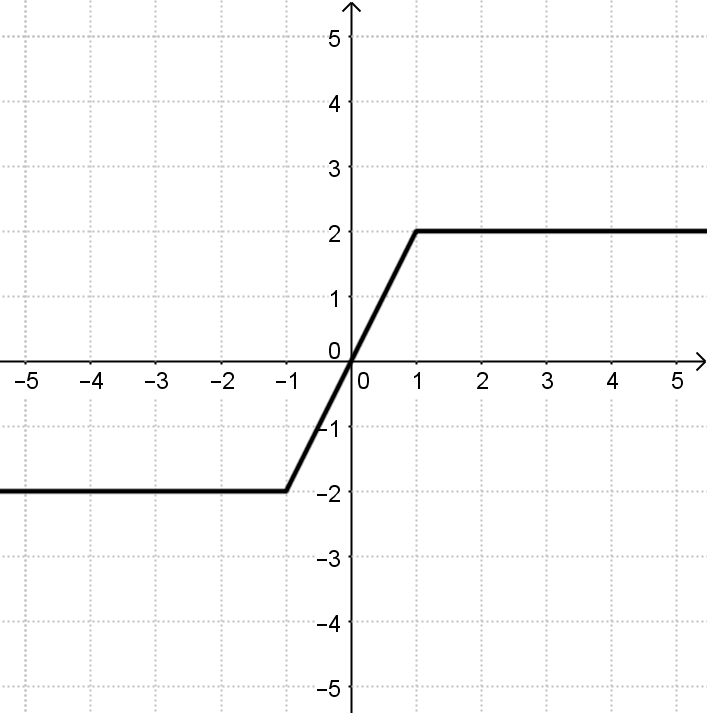
\includegraphics[scale=0.2]{images/522d.png}
	\end{quotation}
	
	\texttt{\tskcol{5.23~~a) (s.)}}
	\begin{quotation}
		\noindent
		Använd definitionen av absolutbelopp (hoppat över ett steg för att det ska vara mer lättläst).
		\[|x-1|=
		\begin{cases}
		x-1&    \text{då } x \ge 1\\
		-(x-1)& \text{då } x < 1
		\end{cases}~~~~~~
		|x-2|=
		\begin{cases}
		x-2&    \text{då } x \ge 2\\
		-(x-2)& \text{då } x < 2
		\end{cases}\]
		Slå samman båda till ett gemensamt uttryck.
		\[|x-1|+|x-2|=
		\begin{cases}
		x-1+x-2&    \text{då } x \ge 2\\
		x-1-(x-2)& \text{då } 1 \le x < 2 \\
		-(x-1)-(x-2)& \text{då } x < 1 
		\end{cases}\]
		\begin{align*}
		    x \ge 2:&~~      x-1+x-2 = 2 \Leftrightarrow x = \frac{5}{2}\\
		1 \le x < 2:&~~    x-1-(x-2) = 2 \Leftrightarrow 1 \neq 2 \Rightarrow \text{ ingen lösning}\\
		      x < 1:&~~ -(x-1)-(x-2) = 2 \Leftrightarrow x = \frac{1}{2}
		\end{align*}
		\\
		\textbf{Svar:} $x = \frac{1}{2}$ eller $x = \frac{5}{2}$
	\end{quotation}
	
	\pagebreak
	\texttt{\tskcol{~~~~~~b) (s.)}}
	\begin{quotation}
		\noindent
		Använd resonemanget från uppgift \texttt{\tskcol{a)}} för intervallen.
		\begin{align*}
		    x \ge 2:&~~      x-1+x-2 = \frac{1}{2} \Leftrightarrow x = \frac{7}{4} \not\ge 2  \Rightarrow\text{falsk lösning}\\
		1 \le x < 2:&~~    x-1-(x-2) = \frac{1}{2} \Leftrightarrow 1 \neq \frac{1}{2} \Rightarrow \text{ ingen lösning}\\
		      x < 1:&~~ -(x-1)-(x-2) = \frac{1}{2} \Leftrightarrow x = \frac{5}{2} \not< 1  \Rightarrow\text{falsk lösning}
		\end{align*}
		\\
		\textbf{Svar:} saknar lösning
	\end{quotation}
	
	\texttt{\tskcol{5.24~~~~ (s.)}}
	\begin{quotation}
		\noindent
		Använd definitionen av absolutbelopp (hoppat över ett steg för att det ska vara mer lättläst).
		\[|x-1|=
		\begin{cases}
		x-1&    \text{då } x \ge 1\\
		-(x-1)& \text{då } x < 1
		\end{cases}~~~~~~
		|x-2|=
		\begin{cases}
		x-2&    \text{då } x \ge 2\\
		-(x-2)& \text{då } x < 2
		\end{cases}\]
		Slå samman båda till ett gemensamt uttryck.
		\[|x-1|+2|x-2|=
		\begin{cases}
		x-1+2(x-2)&    \text{då } x \ge 2\\
		x-1-2(x-2)& \text{då } 1 \le x < 2 \\
		-(x-1)-2(x-2)& \text{då } x < 1 
		\end{cases}\]
		För att lösa uppgiften behöver vi veta värdemängden för varje uttryck och eftersom de är linjär kommer det endast finnas ett värde på $x$ för varje värde på $a$ och ändarna kommer alltid vara minsta respektive största värdet.
		\\ \\
		Värdemängden för första uttrycket ges av $x = 2 \Rightarrow a = 1$ och $x \rightarrow \infty \Rightarrow a \rightarrow \infty$.  
		\\ \\
		Värdemängden för andra uttrycket ges av $x = 1 \Rightarrow a = 2$ och $x \rightarrow 2 \Rightarrow a \rightarrow 1$.  
		\\ \\
		Värdemängden för tredje uttrycket ges av $x \rightarrow -\infty \Rightarrow a \rightarrow \infty$ och $x \rightarrow 1 \Rightarrow a \rightarrow 2$.  
		\\ \\
		För alla $a$ större än 1 kommer det alltså finnas två lösningar.
		\\ \\
		\textbf{Svar:} $a > 1$
	\end{quotation}
	
	\texttt{\tskcol{5.25~~~~ (s.)}}
	\begin{quotation}
		\noindent
		Utnyttja faktumen att $\sqrt{a^2}=|a|$, att $|a| = -a$ eftersom $a < 0$ och att $a^2+b^2 >= 0$ oberoende av värden på $a$ och $b$.
		\begin{align*}
		&\sqrt{a^6+2a^4b^2+a^2b^4}=
		\sqrt{a^2}\sqrt{a^4+2a^2b^2+b^4}=
		|a|\sqrt{(a^2+b^2)^2}= \\ =
		&-a|a^2+b^2|=
		-a(a^2+b^2)
		\end{align*}
		\\
		\textbf{Svar:} $-a(a^2+b^2)$
	\end{quotation}
	
	\texttt{\tskcol{5.26~~~~ (s.)}}
	\begin{quotation}
		\noindent
		Avståndet mellan punkterna i $x$-led kan skrivas som $|x_2-x_1|$ och i $y$-led som $|y_2-y_1|$. Eftersom $x$- och $y$-axeln är vinkelräta mot varandra kan en vinkelrät triangel ritas upp där avståndet mellan punkterna är hypotenusan och avståndet i $x$- respektive $y$-led är kateterna. Pyth. sats säger då att: 
		\begin{align*}
		&d^2=|x_2-x_1|^2+|y_2-y_1|^2 \Leftrightarrow
		d=\varpm\sqrt{|x_2-x_1|^2+|y_2-y_1|^2} \Leftrightarrow \\ \Leftrightarrow
		&d=\sqrt{(x_2-x_1)^2+(y_2-y_1)^2} \text{ V.S.V.}
		\end{align*}
	\end{quotation}
	
	\subsection*{Cirkeln, ellipsen och hyperbeln}
	
	\texttt{\tskcol{5.27~~~~ (s.)}}
	\begin{quotation}
		\noindent
		Kvadratkomplettera och använd sedan cirkelns ekvation för att identifiera medelpunkten och radien.
		\begin{align*}
		&x^2+y^2+2(2x-y)=4 \Leftrightarrow
		x^2+4x+y^2-2y=4 \Leftrightarrow \\ \Leftrightarrow
		&(x+2)^2-2^2+(y-1)^2-1^2=4 \Leftrightarrow \\ \Leftrightarrow
		&(x+2)^2+(y-1)^2=4+4+1 \Leftrightarrow
		(x-(-2))^2+(y-1)^2=3^2
		\end{align*}
		Medelpunkten blir då $(-2,1)$ och radien blir $3$.
		\\ \\
		\textbf{Svar:} medelpunkt: $(-2,1)$, radie: $3$
	\end{quotation}
	
	\texttt{\tskcol{5.28~~~~ (s.)}}
	\begin{quotation}
		\noindent
		Kvadratkomplettera och använd sedan cirkelns ekvation för att identifiera radien.
		\begin{align*}
		&x^2-ax+y^2+2y=a \Leftrightarrow
		(x-\tfrac{a}{2})^2-(\tfrac{a}{2})^2+(y+1)^2-1^2=a \Leftrightarrow \\ \Leftrightarrow
		&(x-\tfrac{a}{2})^2+(y+1)^2=a+\tfrac{a^2}{4}+1
		\end{align*}
		Cirkelns ekvation ger:
		\[r^2=a+\tfrac{a^2}{4}+1, ~~ r=2\]
		\[a+\tfrac{a^2}{4}+1=2^2 \Leftrightarrow
		a^2+4a+4-4*4=0 \Leftrightarrow
		a^2+4a-12=0\]
		pq-formeln:
		\begin{align*}
		&a=-2\pm\sqrt{2^2+12}=-2\pm\sqrt{16}=-2\pm4 \\
		&a_1=2 \\
		&a_2=-6
		\end{align*}
		\\
		\textbf{Svar:} $a_1=2$ eller $a_2=-6$
	\end{quotation}
	
	\pagebreak
	\texttt{\tskcol{5.29~~a) (s.)}}
	\begin{quotation}
		\noindent
		Skriv om ekvationen så den passar ellipsens ekvation och identifiera sedan radien och halvaxlarna.
		\begin{align*}
		&2x^2+(y-1)^2=1 \Leftrightarrow
		\frac{x^2}{\frac{1}{2}}+\left(\frac{y-1}{1}\right)^2=1 \Leftrightarrow \\ \Leftrightarrow
		&\left(\frac{x-0}{\frac{1}{\sqrt{2}}}\right)^2+\left(\frac{y-1}{1}\right)^2=1
		\end{align*}
		radien är $(0,1)$ och halvaxlarna är $\frac{1}{\sqrt{2}}$ och $1$
		\\ \\
		\textbf{Svar:} radie: $(0,1)$, halvaxlar: $\frac{1}{\sqrt{2}}$ och $1$
	\end{quotation}
	
	\texttt{\tskcol{~~~~~~b) (s.)}}
	\begin{quotation}
		\noindent
		Kvadratkomplettera, skriv om ekvationen så den passar ellipsens ekvation och identifiera sedan radien och halvaxlarna.
		\begin{align*}
		&2x^2+y^2-8x+2y+5=0 \Leftrightarrow
		2(x^2-4x)+(y+1)^2-1^2+5=0 \Leftrightarrow \\ \Leftrightarrow
		&2((x-2)^2-2^2)+(y+1)^2+4=0 \Leftrightarrow \\ \Leftrightarrow
		&2(x-2)^2-8+(y+1)^2+4=0 \Leftrightarrow
		2(x-2)^2+(y+1)^2=4 \Leftrightarrow \\ \Leftrightarrow
		&\frac{(x-2)^2}{2}+ \frac{(y+1)^2}{4}=1 \Leftrightarrow
		\left(\frac{x-2}{\sqrt{2}}\right)^2+\left(\frac{y-(-1)}{2}\right)^2=1
		\end{align*}
		radien är $(2,-1)$ och halvaxlarna är $\sqrt{2}$ och $2$
		\\ \\
		\textbf{Svar:} radie: $(2,-1)$, halvaxlar: $\sqrt{2}$ och $2$
	\end{quotation}
	
	\texttt{\tskcol{5.30~~~~ (s.)}}
	\begin{quotation}
		\noindent
		\begin{align*}
		&y^2+2y-4x^2=0 \Leftrightarrow
		(y+1)^2-1^2-(2x)^2=0 \Leftrightarrow \\ \Leftrightarrow
		&(y-(-1))^2-(2(x-0))^2=1
		\end{align*}
		Hyperbelns ekvation ger då att medelpunkten är $(0,-1)$.
		\\ \\
		Kolla sedan vad som händer när $x\rightarrow\infty$ för att bestämma lutningen på asymptoterna.
		\begin{align*}
		&(y-(-1))^2-(2(x-0))^2=1 \Leftrightarrow
		(y+1)^2=(2x)^2+1 \Leftrightarrow \\ \Leftrightarrow
		&y+1=\sqrt{(2x)^2+1} \Rightarrow
		\lim_{x\rightarrow\infty}y=\pm\sqrt{(2x)^2+1}-1 \Leftrightarrow \\ \Leftrightarrow
		&y=\pm\sqrt{(2x)^2}=\pm2x
		\end{align*}
		Lutningen på asymptoterna är alltså $\pm2x$ och eftersom de ska passera igenom medelpunkten blir ekvationen för respektive asymptot $y=2x-1$ samt $y=-2x-1$.
		\\ \\
		\textbf{Svar:} medelpunkt: $(0,-1)$, asymptoter: $y=2x-1$ och $y=-2x-1$
	\end{quotation}
	
	\texttt{\tskcol{5.31~~a) (s.)}}
	\begin{quotation}
		\noindent
		Identifiera vilken andragradskurva det är (\emph{hyperbel} eftersom en av $x$ och $y$ är negativ).
		\begin{align*}
		&x^2-y^2+4x-2y=-2 \Leftrightarrow
		(x+2)^2-2^2-((y+1)^2-1^2)=-2 \Leftrightarrow \\ \Leftrightarrow
		&(x+2)^2-(y+1)^2=1
		\end{align*}
		Medelpunkten är $(-2,-1)$ och eftersom det är $y$-termen som är negativ går linjerna på höger och vänster sida om asymptoterna.
		\\ \\ 
		Lutning på asymptoterna:
		\begin{align*}
		&(x+2)^2-(y+1)^2=1 \Leftrightarrow
		(y+1)^2=(x+2)^2-1 \Rightarrow \\ \Rightarrow
		&\lim_{x\rightarrow\infty}y=\pm\sqrt{(x+2)^2-1}-1 \Leftrightarrow
		y=\pm x
		\end{align*}
		Lutningen på asymptoterna är alltså $\pm x$ och eftersom de ska passera igenom medelpunkten blir ekvationen för respektive asymptot $y=x+1$ samt $y=-x-3$. \\
		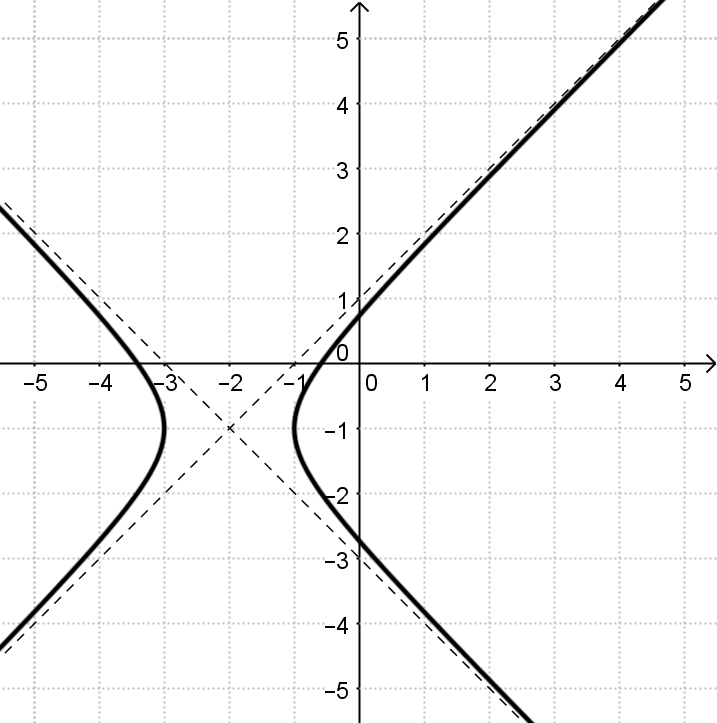
\includegraphics[scale=0.2]{images/531a.png}
	\end{quotation}
	
	\texttt{\tskcol{~~~~~~b) (s.)}}
	\begin{quotation}
		\noindent
		Identifiera vilken andragradskurva det är (\emph{ellips} eftersom $x$ och $y$ är positiva och det är ett ojämnt antal $x^2$- och $y^2$-termer).
		\begin{align*}
		&x^2+2y^2-2x-4y=-1 \Leftrightarrow
		(x-1)^2-1^2+2((y+1)^2-1^2)=-1 \Leftrightarrow \\ \Leftrightarrow
		&(x-1)^2+2(y+1)^2=2 \Leftrightarrow
		\frac{(x-1)^2}{2}+(y+1)^2=1 \Leftrightarrow \\ \Leftrightarrow
		&\left(\frac{x-1}{\sqrt{2}}\right)^2+\left(\frac{y+1}{1}\right)^2=1
		\end{align*}
		Medelpunkten är $(1,1)$ och halvaxlarna är $\sqrt{2}$ och $1$ i $x$- respektive $y$-led. \\
		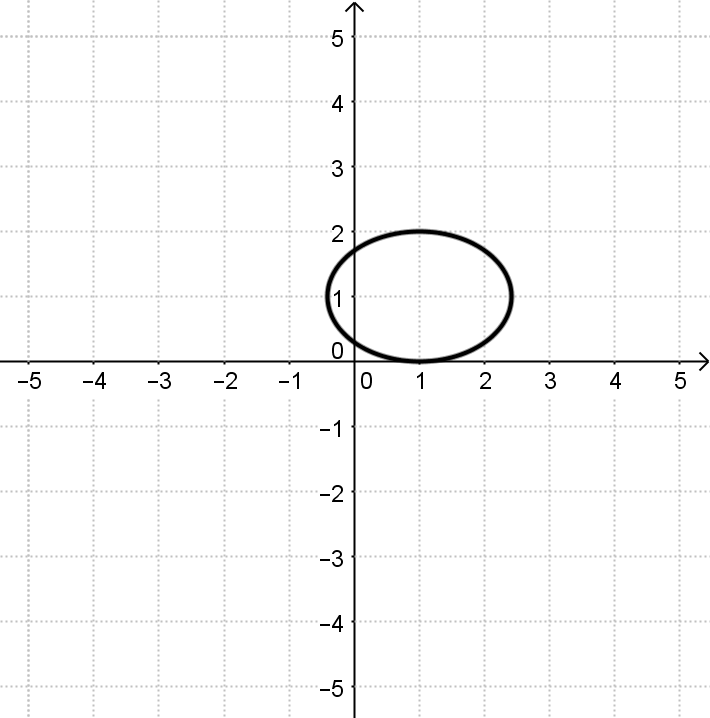
\includegraphics[scale=0.2]{images/531b.png}
	\end{quotation}
	
	\pagebreak
	\texttt{\tskcol{~~~~~~c) (s.)}}
	\begin{quotation}
		\noindent
		Identifiera vilken andragradskurva det är (\emph{liggandes parabel} eftersom att en $y^2$-term men inte en $x^2$-term).
		\begin{align*}
		&y^2-2x-4y+2=0 \Leftrightarrow
		2x=y^2-4y+2 \Leftrightarrow
		2x=(y-2)^2-2^2+2 \Leftrightarrow \\ \Leftrightarrow
		&x=\frac{1}{2}(y-2)^2-1 \Leftrightarrow
		x=\left(\frac{y-2}{\sqrt{2}}\right)^2-1
		\end{align*}
		Vertex är i punkten $(-1,2)$ och eftersom faktorn i $y$-termen är $\frac{1}{\sqrt{2}}$ kommer parabeln bli utdragen med en faktor av det. \\
		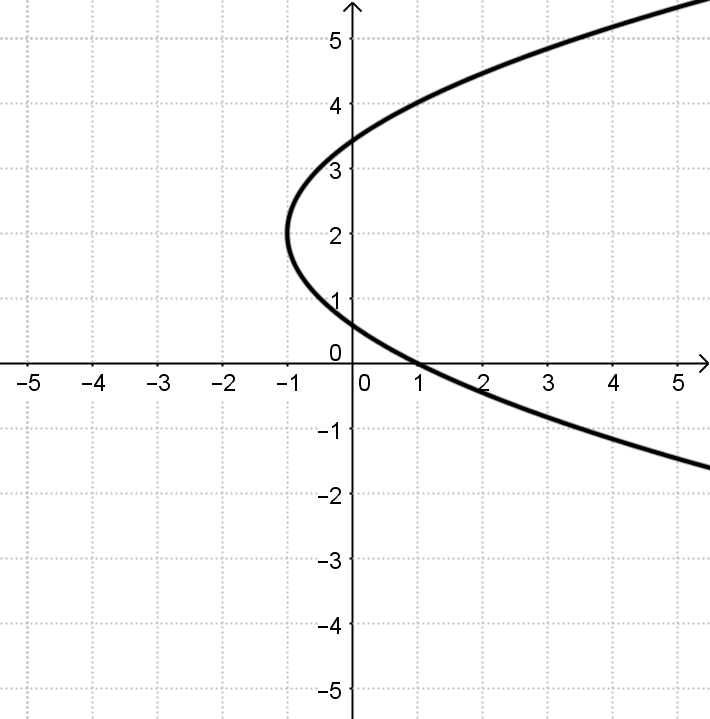
\includegraphics[scale=0.2]{images/531c.png}
	\end{quotation}
	
	\texttt{\tskcol{~~~~~~d) (s.)}}
	\begin{quotation}
		\noindent
		Identifiera vilken andragradskurva det är (\emph{cirkel} eftersom $x$ och $y$ är positiva och det är ett jämnt antal $x^2$- och $y^2$-termer).
		\begin{align*}
		&x^2+y^2+2x+4y+5=0 \Leftrightarrow
		(x+1)^2-1^2+(y+2)^2-2^2+5=0 \Leftrightarrow \\ \Leftrightarrow
		&(x+1)^2+(y+2)^2=0
		\end{align*}
		Medelpunkten är $(-1,-2)$ och radien är $0$ (är en punkt). \\
		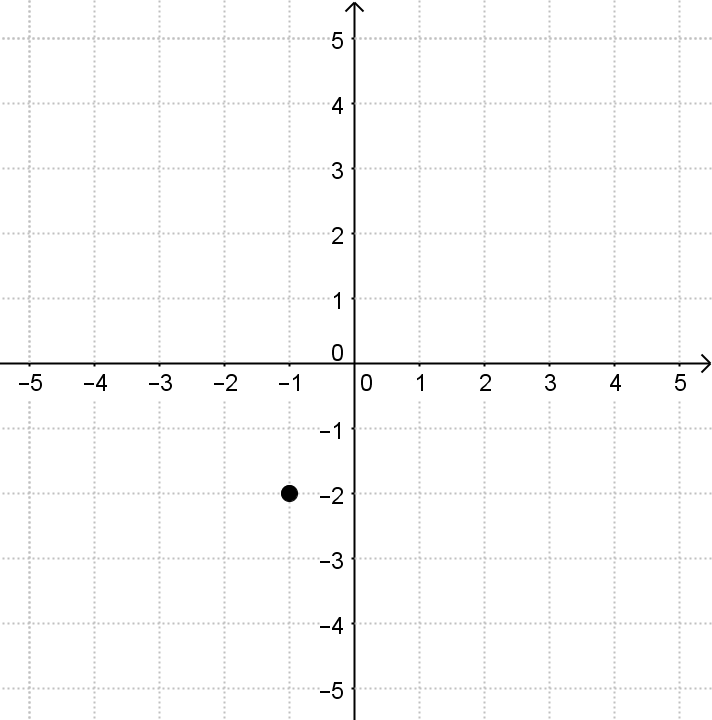
\includegraphics[scale=0.2]{images/531d.png}
	\end{quotation}
	
	\pagebreak
	\texttt{\tskcol{5.32~~~~ (s.)}}
	\begin{quotation}
		\noindent
		Lös det med hjälp av ett ekvationssystem.
		\[\begin{cases}
		x^2+y^2=4 \\
		y=\frac{1}{2}x-1
		\end{cases}\]
		Substitutionsmetoden:
		\begin{align*}
		&x^2+(\tfrac{1}{2}x-1)^2=4 \Leftrightarrow
		x^2+\frac{x^2}{4}-x+1=4 \Leftrightarrow
		\frac{5}{4}x^2-x=3 \Leftrightarrow \\ \Leftrightarrow
		&x^2-\frac{4}{5}x-\frac{12}{5}=0
		\end{align*}
		pq-formeln:
		\begin{align*}
		x=\frac{4}{10}\pm\sqrt{\left(\frac{4}{10}\right)^2+\frac{12}{5}}=
		\frac{4}{10}\pm\sqrt{\frac{16+240}{100}}=
		\frac{4}{10}\pm\frac{16}{10}
		\end{align*}
		\[\begin{cases}
		x_1=2 \Rightarrow y_1=\frac{1}{2}*2-1=0 \\
		x_2=-\frac{6}{5} \Rightarrow y_2=\frac{1}{2}*(-\frac{6}{5})-1=-\frac{16}{10}=-\frac{8}{5}
		\end{cases}\]
		Punkterna är $(2,0)$ och $(-\frac{6}{5},-\frac{8}{5})$.
		\\ \\
		\textbf{Svar:} $(2,0)$ och $(-\frac{6}{5},-\frac{8}{5})$
	\end{quotation}
	
	\texttt{\tskcol{5.33~~~~ (s.)}}
	\begin{quotation}
		\noindent
		Skriv om den räta linjen som $y=kx+m$ med tvåpunktsformeln och använd sen ett ekvationssystem.
		\\ \\
		Tvåpunktsformeln:
		\begin{align*}
		y-1=\frac{4-1}{2+1}(x+1) \Leftrightarrow
		y=\frac{3}{3}(x+1)+1 \Leftrightarrow
		y=x+2
		\end{align*}
		Ekvationssystem:
		\[\begin{cases}
		3x^2-2y^2+6x+4y=3 \\
		y=x+2
		\end{cases}\]
		Substitutionsmetoden:
		\begin{align*}
		&3x^2-2(x+2)^2+6x+4(x+2)=3 \Leftrightarrow \\ \Leftrightarrow
		&3x^2-2(x^2+4x+4)+6x+4x+8=3 \Leftrightarrow \\ \Leftrightarrow
		&3x^2-2x^2-8x-\cancel{8}+10x+\cancel{8}=3 \\
		x^2+2x-3=0
		\end{align*}
		pq-formeln:
		\begin{align*}
		x=-1\pm\sqrt{1^2+3}=
		-1\pm2
		\end{align*}
		\[\begin{cases}
		x_1=1 \Rightarrow y_1=1+2=3 \\
		x_2=-3 \Rightarrow y_2=-3+2=-1
		\end{cases}\]
		Punkterna är $(1,3)$ och $(-3,-1)$.
		\\ \\
		\textbf{Svar:} $(1,3)$ och $(-3,-1)$
	\end{quotation}
	
	\pagebreak
	\section*{Kapitel 6: Komplexa tal}
	
	\texttt{\tskcol{6.1~~~a) (s.)}}
	\begin{quotation}
		\noindent
		$2+3i$ \\
		Re $z = 2$ och Im $z = 3$
		\\ \\
		\textbf{Svar:} $2$, $3$
	\end{quotation}
	
	\texttt{\tskcol{~~~~~~b) (s.)}}
	\begin{quotation}
		\noindent
		$-1-i=-1-1i$ \\
		Re $z = -1$ och Im $z = -1$
		\\ \\
		\textbf{Svar:} $-1$, $-1$
	\end{quotation}
	
	\texttt{\tskcol{~~~~~~c) (s.)}}
	\begin{quotation}
		\noindent
		$3=3+0i$ \\
		Re $z = 3$ och Im $z = 0$
		\\ \\
		\textbf{Svar:} $3$, $0$
	\end{quotation}
	
	\texttt{\tskcol{~~~~~~d) (s.)}}
	\begin{quotation}
		\noindent
		$2i=0+2i$ \\
		Re $z = 0$ och Im $z = 2$
		\\ \\
		\textbf{Svar:} $0$, $2$
	\end{quotation}
	
	\texttt{\tskcol{~~~~~~e) (s.)}}
	\begin{quotation}
		\noindent
		$-i=0+-1i$ \\
		Re $z = 0$ och Im $z = -1$
		\\ \\
		\textbf{Svar:} $0$, $-1$
	\end{quotation}
	
	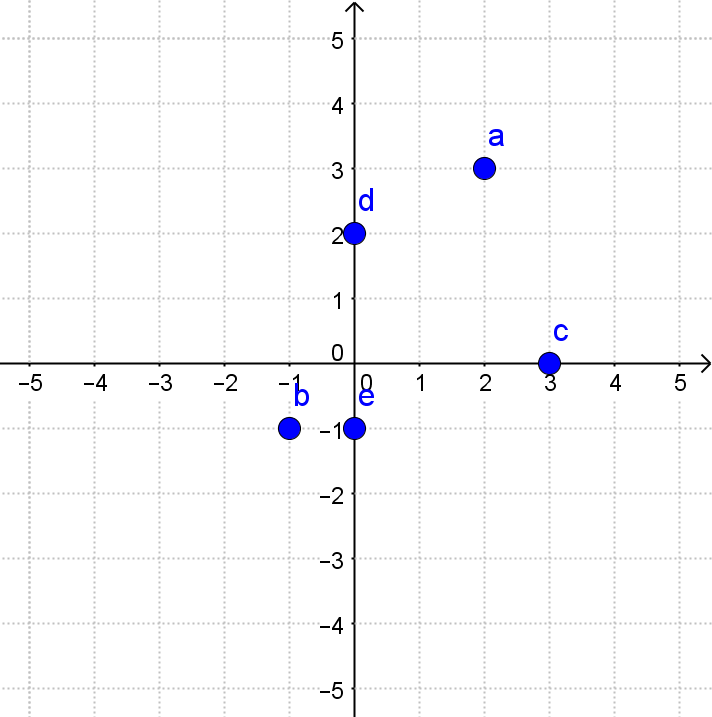
\includegraphics[scale=0.2]{images/61.PNG}
	
	\texttt{\tskcol{6.2~~~a) (s.)}}
	\begin{quotation}
		\noindent
		\[(1+i)+(-3-2i)=(1-3)+(1-2)i=-2-i\]
		\\
		\textbf{Svar:} $-2-i$
	\end{quotation}
	
	\pagebreak
	\texttt{\tskcol{~~~~~~b) (s.)}}
	\begin{quotation}
		\noindent
		\[(1+i)-(3-4i)=(1+i)+(-3+4i)=(1-3)+(1+4)i=-2+4i\]
		\\
		\textbf{Svar:} $-2+4i$
	\end{quotation}
	
	\texttt{\tskcol{~~~~~~c) (s.)}}
	\begin{quotation}
		\noindent
		Använd antingen räkneregeln för multiplikation av komplexa tal eller parentesmultiplikation. \\ \\
		Räkneregel:
		\begin{align*}
		&(1+i)(3-4i)=
		(1+i)(3+(-4)i)=
		(1*3-1*(-4))+(1*(-4)+1*3)i= \\ =
		&(3+4)+(-4+3)i=
		7-i
		\end{align*}
		parentesmultiplikation:
		\begin{align*}
		(1+i)(3-4i)=
		3-4i+3i-4i^2=
		3-i+4=
		7-i
		\end{align*}
		\\
		\textbf{Svar:} $7-i$
	\end{quotation}
	
	\texttt{\tskcol{~~~~~~d) (s.)}}
	\begin{quotation}
		\noindent
		Använd antingen räkneregeln för multiplikation av komplexa tal eller kvadreringsregeln. \\ \\
		Räkneregel:
		\begin{align*}
		&(1-i)^2=
		(1+(-i))(1+(-i))= \\ =
		&(1*1-(-1)*(-1))+(1*(-1)+(-1)*1)i= \\ =
		&(1-1)+(-1-1)i=
		-2i
		\end{align*}
		Kvadreringsregeln:
		\begin{align*}
		(1-i)^2=
		1^2-2i+i^2=
		1-2i-1=
		-2i
		\end{align*}
		\\
		\textbf{Svar:} $-2i$
	\end{quotation}
	
	\pagebreak
	\texttt{\tskcol{~~~~~~e) (s.)}}
	\begin{quotation}
		\noindent
		Använd antingen räkneregeln för multiplikation av komplexa tal eller parentesmultiplikation. \\ \\
		Räkneregel:
		\begin{align*}
		&(5-2i)^3=
		(5+(-2i))(5+(-2i))(5+(-2i))= \\ =
		&((5*5-(-2)*(-2))+(5*(-2)+(-2)*5)i)(5+(-2i))= \\ =
		&((25-4)+(-10-10)i)(5+(-2i))=
		(21+(-20)i)(5+(-2i))= \\ =
		&(21*5-(-20)*(-2))+(21*(-2)+(-20)*5)i= \\ =
		&(105-40)+(-42-100)i= 
		65-142i
		\end{align*}
		parentesmultiplikation:
		\begin{align*}
		&(5-2i)^3=
		5^3-3*5^2*2i+3*5*(2i)^2-(2i)^3= \\ =
		&125-150i-60+8i=
		65-142i
		\end{align*}
		\\
		\textbf{Svar:} $65-142i$
	\end{quotation}
	
	\texttt{\tskcol{~~~~~~f) (s.)}}
	\begin{quotation}
		\noindent
		Uppgift \texttt{\tskcol{d)}} ger att $(x-i)^2=-2i$ (kan också lösas med båda metoderna som tidigare använts).
		\begin{align*}
		(x-i)^4=
		((x-i)^2)^2=
		(-2i)^2=
		4*(-1)=
		-4
		\end{align*}
		\\
		\textbf{Svar:} $-4$
	\end{quotation}
	
	\texttt{\tskcol{6.3~~~a) (s.)}}
	\begin{quotation}
		\noindent
		\[\overline{1+i}=
		1-i\]
		\\
		\textbf{Svar:} $1-i$
	\end{quotation}
	
	\texttt{\tskcol{~~~~~~b) (s.)}}
	\begin{quotation}
		\noindent
		\[\overline{3-5i}=
		3+5i\]
		\\
		\textbf{Svar:} $3+5i$
	\end{quotation}
	
	\texttt{\tskcol{~~~~~~c) (s.)}}
	\begin{quotation}
		\noindent
		\[\overline{-7}=
		-7\]
		\\
		\textbf{Svar:} $-7$
	\end{quotation}
	
	\texttt{\tskcol{~~~~~~d) (s.)}}
	\begin{quotation}
		\noindent
		\[(1+i)\overline{(1+i)}=
		(1+i)(1-i)=
		1^2-2i+i^2=
		-2i\]
		\\
		\textbf{Svar:} $-2i$
	\end{quotation}
	
	\texttt{\tskcol{~~~~~~e) (s.)}}
	\begin{quotation}
		\noindent
		\[|1+i|=
		\sqrt{1^2+1^2}=
		\sqrt{2}\]
		\\
		\textbf{Svar:} $\sqrt{2}$
	\end{quotation}
	
	\texttt{\tskcol{~~~~~~f) (s.)}}
	\begin{quotation}
		\noindent
		\[|i|=
		|0+i|=
		\sqrt{0^2+1^2}=
		1\]
		\\
		\textbf{Svar:} $1$
	\end{quotation}
	
	\texttt{\tskcol{~~~~~~g) (s.)}}
	\begin{quotation}
		\noindent
		\[|3-2i|=
		|3+(-2)i|=
		\sqrt{3^2+(-2)^2}=
		\sqrt{13}\]
		\\
		\textbf{Svar:} $\sqrt{13}$
	\end{quotation}
	
	\texttt{\tskcol{~~~~~~h) (s.)}}
	\begin{quotation}
		\noindent
		\[|-5i|=
		|0+(-5)i|=
		\sqrt{0^2+(-5)^2}=
		5\]
		\\
		\textbf{Svar:} $5$
	\end{quotation}
	
	\texttt{\tskcol{6.4~~~a) (s.)}}
	\begin{quotation}
		\noindent
		Förläng med konjugatet.
		\begin{align*}
		\frac{1}{1+i}=
		\frac{\overline{1+i}}{(1+i)\overline{(1+i)}}=
		\frac{1-i}{(1+i)(1-i)}=
		\frac{1-i}{1^2+1}=
		\frac{1-i}{2}=
		\frac{1}{2}-\frac{1}{2}i
		\end{align*}
		\\
		\textbf{Svar:} $\frac{1}{2}-\frac{1}{2}i$
	\end{quotation}
	
	\texttt{\tskcol{~~~~~~b) (s.)}}
	\begin{quotation}
		\noindent
		Förläng med konjugatet.
		\begin{align*}
		\frac{1}{3-4i}=
		\frac{\overline{3-4i}}{(3-4i)\overline{(3-4i)}}=
		\frac{3+4i}{(3-4i)(3+4i)}=
		\frac{3+4i}{3^2+4^2}=
		\frac{3+4i}{25}=
		\frac{3}{25}+\frac{4}{25}i
		\end{align*}
		\\
		\textbf{Svar:} $\frac{3}{25}+\frac{4}{25}i$
	\end{quotation}
	
	\texttt{\tskcol{~~~~~~c) (s.)}}
	\begin{quotation}
		\noindent
		Förläng med konjugatet.
		\begin{align*}
		&\frac{3-4i}{1+i}=
		\frac{(3-4i)\overline{(1+i)}}{(1+i)\overline{(1+i)}}=
		\frac{(3-4i)(1-i)}{(1+i)(1-i)}=
		\frac{3-3i-4i-4}{1^2+1}= \\ =
		&\frac{-1-7i}{2}=
		-\frac{1}{2}-\frac{7}{2}i
		\end{align*}
		\\
		\textbf{Svar:} $-\frac{1}{2}-\frac{7}{2}i$
	\end{quotation}
	
	\texttt{\tskcol{~~~~~~d) (s.)}}
	\begin{quotation}
		\noindent
		Förläng med konjugatet.
		\begin{align*}
		&\frac{1-i}{1+i}=
		\frac{(1-i)\overline{(1+i)}}{(1+i)\overline{(1+i)}}=
		\frac{(1-i)(1-i)}{(1+i)(1-i)}=
		\frac{1-i-i-1}{1^2+1}= \\ =
		&\frac{-2i}{2}=
		-i
		\end{align*}
		\\
		\textbf{Svar:} $-i$
	\end{quotation}
	
	\texttt{\tskcol{~~~~~~e) (s.)}}
	\begin{quotation}
		\noindent
		Förenkla och förläng med konjugatet.
		\begin{align*}
		&(1+i)^{-2}=
		\frac{1}{(1+i)^2}=
		\frac{1}{1^2+2i+i^2}=
		\frac{1}{2i}= \\ =
		&\frac{\overline{2i}}{2i\overline{2i}}=
		\frac{-2i}{2i(-2i)}=
		\frac{-2i}{4}=
		-\frac{1}{2}i
		\end{align*}
		\\
		\textbf{Svar:} $-\frac{1}{2}i$
	\end{quotation}
	
	\texttt{\tskcol{~~~~~~f) (s.)}}
	\begin{quotation}
		\noindent
		Förläng med konjugatet.
		\begin{align*}
		\frac{1}{i}=
		\frac{\overline{i}}{i\overline{i}}=
		\frac{-i}{-i^2}=
		\frac{-i}{1}=
		-i
		\end{align*}
		\\
		\textbf{Svar:} $-i$
	\end{quotation}
	
	\texttt{\tskcol{6.5~~~a) (s.)}}
	\begin{quotation}
		\noindent
		Använd räknelagen $|zw|=|z||w|$ (upprepade gånger).
		\[|(1-i)^{14}|=
		|1-i|^{14}=
		\sqrt{1^2+(-1)^2}^{14}=
		\sqrt{2}^{14}=
		2^7=
		128\]
		\\
		\textbf{Svar:} $128$
	\end{quotation}
	
	\pagebreak
	\texttt{\tskcol{~~~~~~b) (s.)}}
	\begin{quotation}
		\noindent
		Använd räknelagen $|\frac{z}{w}|=\frac{|z|}{|w|}$.
		\[\left|\frac{3+i}{4+3i}\right|=
		\frac{|3+i|}{|4+3i|}=
		\frac{\sqrt{3^2+1^2}}{\sqrt{4^2+3^2}}=
		\frac{\sqrt{10}}{5}\]
		\\
		\textbf{Svar:} $\frac{\sqrt{10}}{5}$
	\end{quotation}
	
	\texttt{\tskcol{6.6~~~~~ (s.)}}
	\begin{quotation}
		\noindent
		Använd räknelagarna $|zw|=|z||w|$ och $|\frac{z}{w}|=\frac{|z|}{|w|}$.
		\begin{align*}
		&\left|\frac{(1+2i)(7+\sqrt{3}i)^2}{(5+i)^2}\right|=
		\frac{|(1+2i)(7+\sqrt{3}i)^2|}{|(5+i)^2|}=
		\frac{|1+2i||7+\sqrt{3}i|^2}{|5+i|^2}= \\ =
		&\frac{\sqrt{1^2+2^2}\sqrt{7^2+\sqrt{3}^2}^2}{\sqrt{5^2+1^2}^2}=
		\frac{\sqrt{5}*52}{26}=
		2\sqrt{5}
		\end{align*}
		\\
		\textbf{Svar:} $2\sqrt{5}$
	\end{quotation}
	
	\texttt{\tskcol{6.7~~~~~ (s.)}}
	\begin{quotation}
		\noindent
		\\ \\
		\textbf{Svar:}
	\end{quotation}
	
	\texttt{\tskcol{6.8~~~a) (s.)}}
	\begin{quotation}
		\noindent
		\\ \\
		\textbf{Svar:}
	\end{quotation}
	
	\texttt{\tskcol{~~~~~~b) (s.)}}
	\begin{quotation}
		\noindent
		\\ \\
		\textbf{Svar:}
	\end{quotation}
	
	\texttt{\tskcol{6.9~~~~~ (s.)}}
	\begin{quotation}
		\noindent
		\\ \\
		\textbf{Svar:}
	\end{quotation}
	
	\texttt{\tskcol{6.10~~a) (s.)}}
	\begin{quotation}
		\noindent
		\\ \\
		\textbf{Svar:}
	\end{quotation}
	
	\texttt{\tskcol{~~~~~~b) (s.)}}
	\begin{quotation}
		\noindent
		\\ \\
		\textbf{Svar:}
	\end{quotation}
	
	\texttt{\tskcol{~~~~~~c) (s.)}}
	\begin{quotation}
		\noindent
		\\ \\
		\textbf{Svar:}
	\end{quotation}
	
	\texttt{\tskcol{~~~~~~d) (s.)}}
	\begin{quotation}
		\noindent
		\\ \\
		\textbf{Svar:}
	\end{quotation}
	
	\texttt{\tskcol{~~~~~~e) (s.)}}
	\begin{quotation}
		\noindent
		\\ \\
		\textbf{Svar:}
	\end{quotation}
	
	\texttt{\tskcol{6.11~~~~ (s.)}}
	\begin{quotation}
		\noindent
		\\ \\
		\textbf{Svar:}
	\end{quotation}
	
	\texttt{\tskcol{6.12~~a) (s.)}}
	\begin{quotation}
		\noindent
		\\ \\
		\textbf{Svar:}
	\end{quotation}
	
	\texttt{\tskcol{~~~~~~b) (s.)}}
	\begin{quotation}
		\noindent
		\\ \\
		\textbf{Svar:}
	\end{quotation}
	
	\texttt{\tskcol{~~~~~~c) (s.)}}
	\begin{quotation}
		\noindent
		\\ \\
		\textbf{Svar:}
	\end{quotation}
	
	\texttt{\tskcol{~~~~~~d) (s.)}}
	\begin{quotation}
		\noindent
		\\ \\
		\textbf{Svar:}
	\end{quotation}
	
	\texttt{\tskcol{~~~~~~e) (s.)}}
	\begin{quotation}
		\noindent
		\\ \\
		\textbf{Svar:}
	\end{quotation}
	
	\texttt{\tskcol{~~~~~~f) (s.)}}
	\begin{quotation}
		\noindent
		\\ \\
		\textbf{Svar:}
	\end{quotation}
	
	\texttt{\tskcol{~~~~~~g) (s.)}}
	\begin{quotation}
		\noindent
		\\ \\
		\textbf{Svar:}
	\end{quotation}
	
	\texttt{\tskcol{6.13~~~~ (s.)}}
	\begin{quotation}
		\noindent
		\\ \\
		\textbf{Svar:}
	\end{quotation}
	
	\texttt{\tskcol{6.14~~~~ (s.)}}
	\begin{quotation}
		\noindent
		\\ \\
		\textbf{Svar:}
	\end{quotation}
	
	\texttt{\tskcol{6.15~~~~ (s.)}}
	\begin{quotation}
		\noindent
		\\ \\
		\textbf{Svar:}
	\end{quotation}
	
	\texttt{\tskcol{6.16~~~~ (s.)}}
	\begin{quotation}
		\noindent
		\\ \\
		\textbf{Svar:}
	\end{quotation}
	
	\texttt{\tskcol{6.17~~~~ (s.)}}
	\begin{quotation}
		\noindent
		\\ \\
		\textbf{Svar:}
	\end{quotation}
	
	\subsection*{Polär form}
	
	\texttt{\tskcol{6.18~~a) (s.)}}
	\begin{quotation}
		\noindent
		\\ \\
		\textbf{Svar:}
	\end{quotation}
	
	\texttt{\tskcol{~~~~~~b) (s.)}}
	\begin{quotation}
		\noindent
		\\ \\
		\textbf{Svar:}
	\end{quotation}
	
	\texttt{\tskcol{~~~~~~c) (s.)}}
	\begin{quotation}
		\noindent
		\\ \\
		\textbf{Svar:}
	\end{quotation}
	
	\texttt{\tskcol{~~~~~~d) (s.)}}
	\begin{quotation}
		\noindent
		\\ \\
		\textbf{Svar:}
	\end{quotation}
	
	\texttt{\tskcol{~~~~~~e) (s.)}}
	\begin{quotation}
		\noindent
		\\ \\
		\textbf{Svar:}
	\end{quotation}
	
	\texttt{\tskcol{~~~~~~f) (s.)}}
	\begin{quotation}
		\noindent
		\\ \\
		\textbf{Svar:}
	\end{quotation}
	
	\texttt{\tskcol{~~~~~~g) (s.)}}
	\begin{quotation}
		\noindent
		\\ \\
		\textbf{Svar:}
	\end{quotation}
	
	\texttt{\tskcol{6.19~~a) (s.)}}
	\begin{quotation}
		\noindent
		\\ \\
		\textbf{Svar:}
	\end{quotation}
	
	\texttt{\tskcol{~~~~~~b) (s.)}}
	\begin{quotation}
		\noindent
		\\ \\
		\textbf{Svar:}
	\end{quotation}
	
	\texttt{\tskcol{~~~~~~c) (s.)}}
	\begin{quotation}
		\noindent
		\\ \\
		\textbf{Svar:}
	\end{quotation}
	
	\texttt{\tskcol{~~~~~~d) (s.)}}
	\begin{quotation}
		\noindent
		\\ \\
		\textbf{Svar:}
	\end{quotation}
	
	\texttt{\tskcol{~~~~~~e) (s.)}}
	\begin{quotation}
		\noindent
		\\ \\
		\textbf{Svar:}
	\end{quotation}
	
	\texttt{\tskcol{~~~~~~f) (s.)}}
	\begin{quotation}
		\noindent
		\\ \\
		\textbf{Svar:}
	\end{quotation}
	
	\texttt{\tskcol{6.20~~a) (s.)}}
	\begin{quotation}
		\noindent
		\\ \\
		\textbf{Svar:}
	\end{quotation}
	
	\texttt{\tskcol{~~~~~~b) (s.)}}
	\begin{quotation}
		\noindent
		\\ \\
		\textbf{Svar:}
	\end{quotation}
	
	\texttt{\tskcol{~~~~~~c) (s.)}}
	\begin{quotation}
		\noindent
		\\ \\
		\textbf{Svar:}
	\end{quotation}
	
	\texttt{\tskcol{6.21~~a) (s.)}}
	\begin{quotation}
		\noindent
		\\ \\
		\textbf{Svar:}
	\end{quotation}
	
	\texttt{\tskcol{~~~~~~b) (s.)}}
	\begin{quotation}
		\noindent
		\\ \\
		\textbf{Svar:}
	\end{quotation}
	
	\texttt{\tskcol{~~~~~~c) (s.)}}
	\begin{quotation}
		\noindent
		\\ \\
		\textbf{Svar:}
	\end{quotation}
	
	\texttt{\tskcol{6.22~~a) (s.)}}
	\begin{quotation}
		\noindent
		\\ \\
		\textbf{Svar:}
	\end{quotation}
	
	\texttt{\tskcol{~~~~~~b) (s.)}}
	\begin{quotation}
		\noindent
		\\ \\
		\textbf{Svar:}
	\end{quotation}
	
	\texttt{\tskcol{~~~~~~c) (s.)}}
	\begin{quotation}
		\noindent
		\\ \\
		\textbf{Svar:}
	\end{quotation}
	
	\texttt{\tskcol{6.23~~~~ (s.)}}
	\begin{quotation}
		\noindent
		\\ \\
		\textbf{Svar:}
	\end{quotation}
	
	\texttt{\tskcol{6.24~~~~ (s.)}}
	\begin{quotation}
		\noindent
		\\ \\
		\textbf{Svar:}
	\end{quotation}
	
	\texttt{\tskcol{6.25~~~~ (s.)}}
	\begin{quotation}
		\noindent
		\\ \\
		\textbf{Svar:}
	\end{quotation}
	
	\texttt{\tskcol{6.26~~a) (s.)}}
	\begin{quotation}
		\noindent
		\\ \\
		\textbf{Svar:}
	\end{quotation}
	
	\texttt{\tskcol{~~~~~~b) (s.)}}
	\begin{quotation}
		\noindent
		\\ \\
		\textbf{Svar:}
	\end{quotation}
	
	\texttt{\tskcol{~~~~~~c) (s.)}}
	\begin{quotation}
		\noindent
		\\ \\
		\textbf{Svar:}
	\end{quotation}
	
	\texttt{\tskcol{~~~~~~d) (s.)}}
	\begin{quotation}
		\noindent
		\\ \\
		\textbf{Svar:}
	\end{quotation}
	
	\texttt{\tskcol{~~~~~~e) (s.)}}
	\begin{quotation}
		\noindent
		\\ \\
		\textbf{Svar:}
	\end{quotation}
	
	\texttt{\tskcol{~~~~~~f) (s.)}}
	\begin{quotation}
		\noindent
		\\ \\
		\textbf{Svar:}
	\end{quotation}
	
	\texttt{\tskcol{6.27~~~~ (s.)}}
	\begin{quotation}
		\noindent
		\\ \\
		\textbf{Svar:}
	\end{quotation}
	
	\texttt{\tskcol{6.28~~~~ (s.)}}
	\begin{quotation}
		\noindent
		\\ \\
		\textbf{Svar:}
	\end{quotation}
	
	\texttt{\tskcol{6.29~~~~ (s.)}}
	\begin{quotation}
		\noindent
		\\ \\
		\textbf{Svar:}
	\end{quotation}
	
	\texttt{\tskcol{6.30~~~~ (s.)}}
	\begin{quotation}
		\noindent
		\\ \\
		\textbf{Svar:}
	\end{quotation}
	
	\texttt{\tskcol{6.31~~a) (s.)}}
	\begin{quotation}
		\noindent
		\\ \\
		\textbf{Svar:}
	\end{quotation}
	
	\texttt{\tskcol{~~~~~~b) (s.)}}
	\begin{quotation}
		\noindent
		\\ \\
		\textbf{Svar:}
	\end{quotation}
	
	\texttt{\tskcol{6.32~~a) (s.)}}
	\begin{quotation}
		\noindent
		\\ \\
		\textbf{Svar:}
	\end{quotation}
	
	\texttt{\tskcol{~~~~~~b) (s.)}}
	\begin{quotation}
		\noindent
		\\ \\
		\textbf{Svar:}
	\end{quotation}
	
	\texttt{\tskcol{6.33~~~~ (s.)}}
	\begin{quotation}
		\noindent
		\\ \\
		\textbf{Svar:}
	\end{quotation}
	
	\texttt{\tskcol{6.34~~a) (s.)}}
	\begin{quotation}
		\noindent
		\\ \\
		\textbf{Svar:}
	\end{quotation}
	
	\texttt{\tskcol{~~~~~~b) (s.)}}
	\begin{quotation}
		\noindent
		\\ \\
		\textbf{Svar:}
	\end{quotation}
	
	\texttt{\tskcol{~~~~~~c) (s.)}}
	\begin{quotation}
		\noindent
		\\ \\
		\textbf{Svar:}
	\end{quotation}
	
	\texttt{\tskcol{~~~~~~d) (s.)}}
	\begin{quotation}
		\noindent
		\\ \\
		\textbf{Svar:}
	\end{quotation}
	
	\texttt{\tskcol{~~~~~~e) (s.)}}
	\begin{quotation}
		\noindent
		\\ \\
		\textbf{Svar:}
	\end{quotation}
	
	\texttt{\tskcol{6.35~~a) (s.)}}
	\begin{quotation}
		\noindent
		\\ \\
		\textbf{Svar:}
	\end{quotation}
	
	\texttt{\tskcol{~~~~~~b) (s.)}}
	\begin{quotation}
		\noindent
		\\ \\
		\textbf{Svar:}
	\end{quotation}
	
	\texttt{\tskcol{6.36~~~~ (s.)}}
	\begin{quotation}
		\noindent
		\\ \\
		\textbf{Svar:}
	\end{quotation}
	
	\subsection*{Polynomekvationer}
	
	\texttt{\tskcol{6.37~~a) (s.)}}
	\begin{quotation}
		\noindent
		\\ \\
		\textbf{Svar:}
	\end{quotation}
	
	\texttt{\tskcol{~~~~~~b) (s.)}}
	\begin{quotation}
		\noindent
		\\ \\
		\textbf{Svar:}
	\end{quotation}
	
	\texttt{\tskcol{6.38~~a) (s.)}}
	\begin{quotation}
		\noindent
		\\ \\
		\textbf{Svar:}
	\end{quotation}
	
	\texttt{\tskcol{~~~~~~b) (s.)}}
	\begin{quotation}
		\noindent
		\\ \\
		\textbf{Svar:}
	\end{quotation}
	
	\texttt{\tskcol{~~~~~~c) (s.)}}
	\begin{quotation}
		\noindent
		\\ \\
		\textbf{Svar:}
	\end{quotation}
	
	\texttt{\tskcol{6.38~~a) (s.)}}
	\begin{quotation}
		\noindent
		\\ \\
		\textbf{Svar:}
	\end{quotation}
	
	\texttt{\tskcol{~~~~~~b) (s.)}}
	\begin{quotation}
		\noindent
		\\ \\
		\textbf{Svar:}
	\end{quotation}
	
	\texttt{\tskcol{6.40~~~~ (s.)}}
	\begin{quotation}
		\noindent
		\\ \\
		\textbf{Svar:}
	\end{quotation}
	
	\texttt{\tskcol{6.41~~a) (s.)}}
	\begin{quotation}
		\noindent
		\\ \\
		\textbf{Svar:}
	\end{quotation}
	
	\texttt{\tskcol{~~~~~~b) (s.)}}
	\begin{quotation}
		\noindent
		\\ \\
		\textbf{Svar:}
	\end{quotation}
	
	\texttt{\tskcol{~~~~~~c) (s.)}}
	\begin{quotation}
		\noindent
		\\ \\
		\textbf{Svar:}
	\end{quotation}
	
	\texttt{\tskcol{~~~~~~d) (s.)}}
	\begin{quotation}
		\noindent
		\\ \\
		\textbf{Svar:}
	\end{quotation}
	
	\texttt{\tskcol{~~~~~~e) (s.)}}
	\begin{quotation}
		\noindent
		\\ \\
		\textbf{Svar:}
	\end{quotation}
	
	\texttt{\tskcol{~~~~~~f) (s.)}}
	\begin{quotation}
		\noindent
		\\ \\
		\textbf{Svar:}
	\end{quotation}
	
	\texttt{\tskcol{6.42~~~~ (s.)}}
	\begin{quotation}
		\noindent
		\\ \\
		\textbf{Svar:}
	\end{quotation}
	
	\texttt{\tskcol{6.43~~~~ (s.)}}
	\begin{quotation}
		\noindent
		\\ \\
		\textbf{Svar:}
	\end{quotation}
	
	\texttt{\tskcol{6.44~~~~ (s.)}}
	\begin{quotation}
		\noindent
		\\ \\
		\textbf{Svar:}
	\end{quotation}
	
	\texttt{\tskcol{6.45~~~~ (s.)}}
	\begin{quotation}
		\noindent
		\\ \\
		\textbf{Svar:}
	\end{quotation}
	
	\texttt{\tskcol{6.46~~~~ (s.)}}
	\begin{quotation}
		\noindent
		\\ \\
		\textbf{Svar:}
	\end{quotation}
	
	\texttt{\tskcol{6.47~~a) (s.)}}
	\begin{quotation}
		\noindent
		\\ \\
		\textbf{Svar:}
	\end{quotation}
	
	\texttt{\tskcol{~~~~~~b) (s.)}}
	\begin{quotation}
		\noindent
		\\ \\
		\textbf{Svar:}
	\end{quotation}
	
	\texttt{\tskcol{~~~~~~c) (s.)}}
	\begin{quotation}
		\noindent
		\\ \\
		\textbf{Svar:}
	\end{quotation}
	
	\texttt{\tskcol{6.48~~~~ (s.)}}
	\begin{quotation}
		\noindent
		\\ \\
		\textbf{Svar:}
	\end{quotation}
	
	\texttt{\tskcol{6.49~~~~ (s.)}}
	\begin{quotation}
		\noindent
		\\ \\
		\textbf{Svar:}
	\end{quotation}
	
	\texttt{\tskcol{6.50~~~~ (s.)}}
	\begin{quotation}
		\noindent
		\\ \\
		\textbf{Svar:}
	\end{quotation}
	
	\texttt{\tskcol{6.51~~~~ (s.)}}
	\begin{quotation}
		\noindent
		\\ \\
		\textbf{Svar:}
	\end{quotation}
	
	\texttt{\tskcol{6.52~~a) (s.)}}
	\begin{quotation}
		\noindent
		\\ \\
		\textbf{Svar:}
	\end{quotation}
	
	\texttt{\tskcol{~~~~~~b) (s.)}}
	\begin{quotation}
		\noindent
		\\ \\
		\textbf{Svar:}
	\end{quotation}
	
	\texttt{\tskcol{~~~~~~c) (s.)}}
	\begin{quotation}
		\noindent
		\\ \\
		\textbf{Svar:}
	\end{quotation}
	
	\texttt{\tskcol{~~~~~~d) (s.)}}
	\begin{quotation}
		\noindent
		\\ \\
		\textbf{Svar:}
	\end{quotation}
	
	\texttt{\tskcol{6.53~~~~ (s.)}}
	\begin{quotation}
		\noindent
		\\ \\
		\textbf{Svar:}
	\end{quotation}
	
	\texttt{\tskcol{6.54~~~~ (s.)}}
	\begin{quotation}
		\noindent
		\\ \\
		\textbf{Svar:}
	\end{quotation}
	
	\subsection*{Blandade problem}
	
	\texttt{\tskcol{6.55~~a) (s.)}}
	\begin{quotation}
		\noindent
		\\ \\
		\textbf{Svar:}
	\end{quotation}
	
	\texttt{\tskcol{~~~~~~b) (s.)}}
	\begin{quotation}
		\noindent
		\\ \\
		\textbf{Svar:}
	\end{quotation}
	
	\texttt{\tskcol{6.56~~~~ (s.)}}
	\begin{quotation}
		\noindent
		\\ \\
		\textbf{Svar:}
	\end{quotation}
	
	\texttt{\tskcol{6.57~~a) (s.)}}
	\begin{quotation}
		\noindent
		\\ \\
		\textbf{Svar:}
	\end{quotation}
	
	\texttt{\tskcol{~~~~~~b) (s.)}}
	\begin{quotation}
		\noindent
		\\ \\
		\textbf{Svar:}
	\end{quotation}
	
	\texttt{\tskcol{6.58~~~~ (s.)}}
	\begin{quotation}
		\noindent
		\\ \\
		\textbf{Svar:}
	\end{quotation}
	
	\texttt{\tskcol{6.59~~~~ (s.)}}
	\begin{quotation}
		\noindent
		\\ \\
		\textbf{Svar:}
	\end{quotation}
	
	\texttt{\tskcol{6.60~~~~ (s.)}}
	\begin{quotation}
		\noindent
		\\ \\
		\textbf{Svar:}
	\end{quotation}
	
	\texttt{\tskcol{6.61~~a) (s.)}}
	\begin{quotation}
		\noindent
		\\ \\
		\textbf{Svar:}
	\end{quotation}
	
	\texttt{\tskcol{~~~~~~b) (s.)}}
	\begin{quotation}
		\noindent
		\\ \\
		\textbf{Svar:}
	\end{quotation}
	
	\texttt{\tskcol{~~~~~~c) (s.)}}
	\begin{quotation}
		\noindent
		\\ \\
		\textbf{Svar:}
	\end{quotation}
	
	\texttt{\tskcol{~~~~~~d) (s.)}}
	\begin{quotation}
		\noindent
		\\ \\
		\textbf{Svar:}
	\end{quotation}
	
	\texttt{\tskcol{6.62~~a) (s.)}}
	\begin{quotation}
		\noindent
		\\ \\
		\textbf{Svar:}
	\end{quotation}
	
	\texttt{\tskcol{~~~~~~b) (s.)}}
	\begin{quotation}
		\noindent
		\\ \\
		\textbf{Svar:}
	\end{quotation}
	
	\texttt{\tskcol{~~~~~~c) (s.)}}
	\begin{quotation}
		\noindent
		\\ \\
		\textbf{Svar:}
	\end{quotation}
	
	\texttt{\tskcol{~~~~~~d) (s.)}}
	\begin{quotation}
		\noindent
		\\ \\
		\textbf{Svar:}
	\end{quotation}
	
	\texttt{\tskcol{6.63~~~~ (s.)}}
	\begin{quotation}
		\noindent
		\\ \\
		\textbf{Svar:}
	\end{quotation}
	
	\texttt{\tskcol{6.64~~~~ (s.)}}
	\begin{quotation}
		\noindent
		\\ \\
		\textbf{Svar:}
	\end{quotation}
	
	\texttt{\tskcol{6.65~~~~ (s.)}}
	\begin{quotation}
		\noindent
		\\ \\
		\textbf{Svar:}
	\end{quotation}
	
	\texttt{\tskcol{6.66~~~~ (s.)}}
	\begin{quotation}
		\noindent
		\\ \\
		\textbf{Svar:}
	\end{quotation}
	
	\texttt{\tskcol{6.67~~~~ (s.)}}
	\begin{quotation}
		\noindent
		\\ \\
		\textbf{Svar:}
	\end{quotation}
	
	\texttt{\tskcol{6.68~~a) (s.)}}
	\begin{quotation}
		\noindent
		\\ \\
		\textbf{Svar:}
	\end{quotation}
	
	\texttt{\tskcol{~~~~~~b) (s.)}}
	\begin{quotation}
		\noindent
		\\ \\
		\textbf{Svar:}
	\end{quotation}
	
	\texttt{\tskcol{~~~~~~c) (s.)}}
	\begin{quotation}
		\noindent
		\\ \\
		\textbf{Svar:}
	\end{quotation}
\end{document}